\title{数列（2016--2025 高考真题）}
\author{}
\date{}
\maketitle
\noindent 本专题共 125 道题，按年份排列。每题标注原卷与原题号。

\section*{2016 年}

\begin{question}[points=12]
\textbf{来源：}2016 年 全国III卷-理科，第 17 题\par
已知数列 $\{a_n\}$ 的前 $n$ 项和 $S_n=1+\lambda a_n$, 其中 $\lambda\ne 0$.

(1) 证明 $\{a_n\}$ 是等比数列, 并求其通项公式;

(2) 若 $S_5=\frac{31}{32}$, 求 $\lambda$.
\begin{solution}

\textbf{分析：}(1) 根据数列通项公式与前 $n$ 项和公式之间的关系进行递推, 结合等比数列的定义进行证明求解. (2) 根据条件建立方程关系进行求解.

\textbf{详解：}(1) $\because S_n=1+\lambda a_n$, $\lambda\ne0$. $\therefore a_n\ne0$. 当 $n\ge2$ 时, $a_n=S_n-S_{n-1}=1+\lambda a_n-1-\lambda a_{n-1}=\lambda a_n-\lambda a_{n-1}$, 即 $(\lambda-1)a_n=\lambda a_{n-1}$, $\because\lambda\ne0,a_n\ne0$, $\therefore\lambda-1\ne0$, 即 $\lambda\ne1$, $\therefore\frac{a_n}{a_{n-1}}=\frac{\lambda}{\lambda-1}$ ($n\ge2$). $\therefore\{a_n\}$ 是等比数列, 公比 $q=\frac{\lambda}{\lambda-1}$. 当 $n=1$ 时, $S_1=1+\lambda a_1=a_1$, $\therefore a_1=\frac{1}{1-\lambda}$, $\therefore a_n=\frac{1}{1-\lambda}\cdot(\frac{\lambda}{\lambda-1})^{n-1}$.
(2) 若 $S_5=\frac{31}{32}$, 则 $S_5=1+\lambda[\frac{1}{1-\lambda}\cdot(\frac{\lambda}{\lambda-1})^4]=\frac{31}{32}$, 即 $(\frac{\lambda}{\lambda-1})^5=\frac{31}{32}-1=-\frac{1}{32}$, $\therefore\frac{\lambda}{\lambda-1}=-\frac{1}{2}$, 得 $\lambda=-1$.
\end{solution}
\end{question}

\begin{question}[points=12]
\textbf{来源：}2016 年 全国III卷-文科，第 17 题\par
已知各项都为正数的数列 $\{a_n\}$ 满足 $a_1=1$, $a_n^2-(2a_{n+1}-1)a_n-2a_{n+1}=0$. 

(1) 求 $a_2$, $a_3$; 

(2) 求 $\{a_n\}$ 的通项公式.
\begin{solution}
\textbf{答案：}见解析

\textbf{分析：}(1) 根据题意, 由数列的递推公式, 令 $n=1$ 可得 $a_1^2-(2a_2-1)a_1-2a_2=0$, 将 $a_1=1$ 代入可得 $a_2$ 的值, 进而令 $n=2$ 可得 $a_2^2-(2a_3-1)a_2-2a_3=0$, 将 $a_2=\dfrac{1}{2}$ 代入计算可得 $a_3$ 的值, 即可得答案; (2) 将 $a_n^2-(2a_{n+1}-1)a_n-2a_{n+1}=0$ 变形可得 $(a_n-2a_{n+1})(a_n+1)=0$, 进而分析可得 $a_n=2a_{n+1}$ 或 $a_n=-1$, 结合数列各项为正可得 $a_n=2a_{n+1}$, 结合等比数列的性质可得 $\{a_n\}$ 是首项为 $a_1=1$, 公比为 $\dfrac{1}{2}$ 的等比数列, 由等比数列的通项公式计算可得答案.

\textbf{详解：}(1) 当 $n=1$ 时, $a_1^2-(2a_2-1)a_1-2a_2=0$, $a_1=1$, 则 $1-(2a_2-1)-2a_2=0$, 解得 $a_2=\dfrac{1}{2}$.
当 $n=2$ 时, $a_2^2-(2a_3-1)a_2-2a_3=0$, 由 $a_2=\dfrac{1}{2}$ 得 $\dfrac{1}{4}-(2a_3-1)\cdot\dfrac{1}{2}-2a_3=0$, 解得 $a_3=\dfrac{1}{4}$.
故 $a_2=\dfrac{1}{2}$, $a_3=\dfrac{1}{4}$.
(2) 由 $a_n^2-(2a_{n+1}-1)a_n-2a_{n+1}=0$ 得 $(a_n-2a_{n+1})(a_n+1)=0$, 因为 $\{a_n\}$ 各项都为正数, 所以 $a_n=2a_{n+1}$, 即 $\dfrac{a_{n+1}}{a_n}=\dfrac{1}{2}$. 故数列 $\{a_n\}$ 是首项为 $1$, 公比为 $\dfrac{1}{2}$ 的等比数列, 所以 $a_n=1\times\left(\dfrac{1}{2}\right)^{n-1}=\left(\dfrac{1}{2}\right)^{n-1}$.
\end{solution}
\end{question}

\begin{question}[points=12]
\textbf{来源：}2016 年 全国II卷-理科，第 17 题\par
$S_n$为等差数列$\{a_n\}$的前$n$项和，且$a_1=1$，$S_7=28$，记$b_n=[\lg a_n]$，其中$[x]$表示不超过$x$的最大整数，如$[0.9]=0$，$[\lg 99]=1$．

（Ⅰ）求$b_1$，$b_{11}$，$b_{101}$；

（Ⅱ）求数列$\{b_n\}$的前$1000$项和．
\begin{solution}
\textbf{答案：}（Ⅰ）$b_1=0$，$b_{11}=1$，$b_{101}=2$；（Ⅱ）1893

\textbf{分析：}（Ⅰ）利用已知条件求出等差数列的公差，求出通项公式，然后求解$b_1$，$b_{11}$，$b_{101}$；（Ⅱ）找出数列的规律，然后求数列$\{b_n\}$的前$1000$项和．

\textbf{详解：}（Ⅰ）设公差为$d$，$S_7=7a_4=28$，$a_4=4$，$d=1$，$a_n=n$，$b_n=[\lg n]$，$b_1=[\lg 1]=0$，$b_{11}=[\lg 11]=1$，$b_{101}=[\lg 101]=2$．
（Ⅱ）$b_1=b_2=\ldots=b_9=0$，$b_{10}=b_{11}=\ldots=b_{99}=1$，$b_{100}=b_{101}=\ldots=b_{999}=2$，$b_{1000}=3$，前1000项和为$9\times0+90\times1+900\times2+3=1893$．
\end{solution}
\end{question}

\begin{question}[points=12]
\textbf{来源：}2016 年 全国II卷-文科，第 17 题\par
等差数列$\{a_n\}$中，$a_3+a_4=4$，$a_5+a_7=6$。

（Ⅰ）求$\{a_n\}$的通项公式；

（Ⅱ）设$b_n=[a_n]$，求数列$\{b_n\}$的前10项和，其中$[x]$表示不超过$x$的最大整数，如$[0.9]=0$，$[2.6]=2$。
\begin{solution}
\textbf{答案：}（Ⅰ）$a_n=\frac{2n-3}{5}$；（Ⅱ）24

\textbf{分析：}（Ⅰ）设公差$d$，$a_3+a_4=2a_1+5d=4$，$a_5+a_7=2a_1+10d=6$，解得$a_1=\frac{1}{5}$，$d=\frac{2}{5}$，$a_n=\frac{2n-3}{5}$。
（Ⅱ）$b_n=[a_n]$，计算前10项得$b_1=b_2=b_3=1$，$b_4=b_5=2$，$b_6=b_7=b_8=3$，$b_9=b_{10}=4$，和$=3\times1+2\times2+3\times3+2\times4=24$。
\end{solution}
\end{question}

\begin{question}[points=5]
\textbf{来源：}2016 年 全国I卷-理科，第 3 题\par
已知等差数列$\{a_n\}$前9项的和为27，$a_{10}=8$，则$a_{100}=$（ ）
\begin{choices}
  \item $100$
  \item $99$
  \item $98$
  \item $97$
\end{choices}
\begin{solution}
\textbf{答案：}C

\textbf{分析：}根据已知可得$a_5=3$，进而求出公差，可得答案．

\textbf{详解：}解：因为等差数列$\{a_n\}$前9项的和为27，$S_9=\frac{9(a_1+a_9)}{2}=9a_5$．所以$9a_5=27$，$a_5=3$，又因为$a_{10}=8$，所以$d=1$，所以$a_{100}=a_5+95d=98$，故选：C．
\end{solution}
\end{question}

\begin{question}[points=5]
\textbf{来源：}2016 年 全国I卷-理科，第 15 题\par
设等比数列$\{a_n\}$满足$a_1+a_3=10$，$a_2+a_4=5$，则$a_1a_2\cdots a_n$的最大值为．
\fillin[{$64$}]
\begin{solution}
\textbf{答案：}$64$

\textbf{分析：}求出数列的等比与首项，化简$a_1a_2\cdots a_n$，然后求解最值．

\textbf{详解：}解：等比数列$\{a_n\}$满足$a_1+a_3=10$，$a_2+a_4=5$，可得$q(a_1+a_3)=5$，解得$q=\frac{1}{2}$．$a_1+q^2a_1=10$，解得$a_1=8$．则$a_1a_2\cdots a_n=a_1^n q^{1+2+3+\cdots+(n-1)}=8^n \left(\frac{1}{2}\right)^{\frac{n(n-1)}{2}}=2^{3n-\frac{n(n-1)}{2}}=2^{\frac{-n^2+7n}{2}}$，当$n=3$或$4$时，表达式取得最大值：$2^{\frac{-9+21}{2}}=2^6=64$．故答案为：$64$．
\end{solution}
\end{question}

\begin{question}[points=12]
\textbf{来源：}2016 年 全国I卷-文科，第 17 题\par
已知$\{a_n\}$是公差为3的等差数列，数列$\{b_n\}$满足$b_1=1$，$b_2=\frac{1}{3}$，$a_nb_{n+1}+b_{n+1}=nb_n$。

（Ⅰ）求$\{a_n\}$的通项公式；

（Ⅱ）求$\{b_n\}$的前$n$项和。
\begin{solution}
\textbf{答案：}（Ⅰ）$a_n=3n-1$；（Ⅱ）$S_n=\frac{3}{2}(1-3^{-n})=\frac{3}{2}-\frac{1}{2\cdot3^{n-1}}$

\textbf{分析：}（Ⅰ）令$n=1$，可得$a_1=2$，结合$\{a_n\}$是公差为3的等差数列，可得$\{a_n\}$的通项公式；
（Ⅱ）由（Ⅰ）可得：数列$\{b_n\}$是以1为首项，以$\frac{1}{3}$为公比的等比数列，进而可得$\{b_n\}$的前$n$项和。

\textbf{详解：}（Ⅰ）$\because a_nb_{n+1}+b_{n+1}=nb_n$。当$n=1$时，$a_1b_2+b_2=b_1$。$\because b_1=1$，$b_2=\frac{1}{3}$，$\therefore a_1=2$，又$\because \{a_n\}$是公差为3的等差数列，$\therefore a_n=3n-1$。
（Ⅱ）由（I）知：$(3n-1)b_{n+1}+b_{n+1}=nb_n$，即$3b_{n+1}=b_n$。即数列$\{b_n\}$是以1为首项，以$\frac{1}{3}$为公比的等比数列，$\therefore \{b_n\}$的前$n$项和$S_n=\frac{1\times(1-(\frac{1}{3})^n)}{1-\frac{1}{3}}=\frac{3}{2}(1-3^{-n})=\frac{3}{2}-\frac{1}{2\cdot3^{n-1}}$。
\end{solution}
\end{question}

\section*{2017 年}

\begin{question}[points=5]
\textbf{来源：}2017 年 全国III卷-理科，第 9 题\par
等差数列$\{a_n\}$的首项为$1$，公差不为$0$．若$a_2$，$a_3$，$a_6$成等比数列，则$\{a_n\}$前$6$项的和为（ ）
\begin{choices}
  \item $-24$
  \item $-3$
  \item $3$
  \item $8$
\end{choices}
\begin{solution}
\textbf{答案：}$A$

\textbf{分析：}利用等差数列通项公式、等比数列性质列出方程，求出公差，由此能求出$\{a_n\}$前6项的和。

\textbf{详解：}因为等差数列$\{a_n\}$的首项为$1$，公差不为$0$．$a_2$，$a_3$，$a_6$成等比数列，所以$a_3^2=a_2\cdot a_6$，所以$(a_1+2d)^2=(a_1+d)(a_1+5d)$，且$a_1=1$，$d\neq0$，解得$d=-2$，所以$\{a_n\}$前$6$项的和为$S_6=6\times1+\frac{6\times5}{2}\times(-2)=6-30=-24$。故选A。
\end{solution}
\end{question}

\begin{question}[points=5]
\textbf{来源：}2017 年 全国III卷-理科，第 14 题\par
设等比数列$\{a_n\}$满足$a_1+a_2=-1$，$a_1-a_3=-3$，则$a_4=$．
\fillin[{$-8$}]
\begin{solution}
\textbf{答案：}$-8$

\textbf{分析：}设等比数列$\{a_n\}$的公比为$q$，由$a_1+a_2=-1$，$a_1-a_3=-3$，可得：$a_1(1+q)=-1$，$a_1(1-q^2)=-3$，解出即可得出。

\textbf{详解：}设等比数列$\{a_n\}$的公比为$q$，因为$a_1+a_2=-1$，$a_1-a_3=-3$，所以$a_1(1+q)=-1$，$a_1(1-q^2)=-3$，解得$a_1=1$，$q=-2$．则$a_4=(-2)^3=-8$。故答案为：$-8$。
\end{solution}
\end{question}

\begin{question}[points=12]
\textbf{来源：}2017 年 全国III卷-文科，第 17 题\par
设数列$\{a_n\}$满足$a_1+3a_2+\cdots+(2n-1)a_n=2n$。

（1）求$\{a_n\}$的通项公式；

（2）求数列$\{\frac{a_n}{2n+1}\}$的前$n$项和。
\begin{solution}
\textbf{答案：}（1）$a_n=\frac{2}{2n-1}$；（2）$\frac{2n}{2n+1}$

\textbf{分析：}（1）利用数列递推关系即可得出。（2）利用裂项求和方法即可得出。

\textbf{详解：}（1）当$n\ge 2$时，$a_1+3a_2+\cdots+(2n-3)a_{n-1}=2(n-1)$，与原式相减得$(2n-1)a_n=2$，所以$a_n=\frac{2}{2n-1}$，当$n=1$时$a_1=2$也满足。
（2）$\frac{a_n}{2n+1}=\frac{2}{(2n-1)(2n+1)}=\frac{1}{2n-1}-\frac{1}{2n+1}$，所以前$n$项和为$1-\frac{1}{2n+1}=\frac{2n}{2n+1}$。
\end{solution}
\end{question}

\begin{question}[points=5]
\textbf{来源：}2017 年 全国II卷-理科，第 3 题\par
我国古代数学名著《算法统宗》中有如下问题：“远看巍巍塔七层，红光点点倍加增，共灯三百八十一，请问尖头几盏灯？”意思是：一座 $7$ 层塔共挂了 $381$ 盏灯，且相邻两层中的下一层灯数是上一层灯数的 $2$ 倍，则塔的顶层共有灯（   ）
\begin{choices}
  \item $1$ 盏
  \item $3$ 盏
  \item $5$ 盏
  \item $9$ 盏
\end{choices}
\begin{solution}
\textbf{答案：}$B$

\textbf{分析：}设塔顶的 $a_1$ 盏灯，由题意 $\{a_n\}$ 是公比为 $2$ 的等比数列，利用等比数列前 $n$ 项和公式列出方程，能求出结果。

\textbf{详解：}设塔顶的 $a_1$ 盏灯，由题意 $\{a_n\}$ 是公比为 $2$ 的等比数列，$\therefore S_7=\frac{a_1(1-2^7)}{1-2}=381$，解得 $a_1=3$．故选：$B$。
\end{solution}
\end{question}

\begin{question}[points=5]
\textbf{来源：}2017 年 全国II卷-理科，第 15 题\par
等差数列 $\{a_n\}$ 的前 $n$ 项和为 $S_n$，$a_3=3$，$S_4=10$，则 $\sum_{k=1}^{n}\frac{1}{S_k}=$ ．
\fillin[{$\frac{2n}{n+1}$}]
\begin{solution}
\textbf{答案：}$\frac{2n}{n+1}$

\textbf{分析：}利用已知条件求出等差数列的前 $n$ 项和，然后化简所求的表达式，求解即可。

\textbf{详解：}等差数列 $\{a_n\}$ 的前 $n$ 项和为 $S_n$，$a_3=3$，$S_4=10$，$S_4=2(a_2+a_3)=10$，可得 $a_2=2$，数列的首项为 $1$，公差为 $1$，$S_n=\frac{n(n+1)}{2}$，$\frac{1}{S_k}=\frac{2}{k(k+1)}=2(\frac{1}{k}-\frac{1}{k+1})$，则 $\sum_{k=1}^{n}\frac{1}{S_k}=2[1-\frac{1}{2}+\frac{1}{2}-\frac{1}{3}+\cdots+\frac{1}{n}-\frac{1}{n+1}]=2(1-\frac{1}{n+1})=\frac{2n}{n+1}$．故答案为：$\frac{2n}{n+1}$。
\end{solution}
\end{question}

\begin{question}[points=12]
\textbf{来源：}2017 年 全国II卷-文科，第 17 题\par
已知等差数列 $\{a_n\}$ 的前 $n$ 项和为 $S_n$, 等比数列 $\{b_n\}$ 的前 $n$ 项和为 $T_n$, $a_1=-1$, $b_1=1$, $a_2+b_2=2$. \\ (1) 若 $a_3+b_3=5$, 求 $\{b_n\}$ 的通项公式; \\ (2) 若 $T_3=21$, 求 $S_3$.
\begin{solution}

\textbf{分析：}(1) 设等差数列 $\{a_n\}$ 的公差为 $d$, 等比数列 $\{b_n\}$ 的公比为 $q$, 运用等差数列和等比数列的通项公式, 列方程解方程可得 $d$, $q$, 即可得到所求通项公式; (2) 运用等比数列的求和公式, 解方程可得公比, 再由等差数列的通项公式和求和, 计算即可得到所求和.

\textbf{详解：}(1) 设等差数列 $\{a_n\}$ 的公差为 $d$, 等比数列 $\{b_n\}$ 的公比为 $q$, $a_1=-1$, $b_1=1$, $a_2+b_2=2$, $a_3+b_3=5$, 可得 $-1+d+q=2$, $-1+2d+q^2=5$, 解得 $d=1$, $q=2$ 或 $d=3$, $q=0$ (舍去), 则 $\{b_n\}$ 的通项公式为 $b_n=2^{n-1}$, $n\in\mathbb{N}^*$; \\ (2) $b_1=1$, $T_3=21$, 可得 $1+q+q^2=21$, 解得 $q=4$ 或 $-5$, 当 $q=4$ 时, $b_2=4$, $a_2=2-4=-2$, $d=-2-(-1)=-1$, $S_3=-1-2-3=-6$; 当 $q=-5$ 时, $b_2=-5$, $a_2=2-(-5)=7$, $d=7-(-1)=8$, $S_3=-1+7+15=21$.
\end{solution}
\end{question}

\begin{question}[points=5]
\textbf{来源：}2017 年 全国I卷-理科，第 4 题\par
记 $S_n$ 为等差数列 $\{a_n\}$ 的前 $n$ 项和．若 $a_4+a_5=24$，$S_6=48$，则 $\{a_n\}$ 的公差为（ ）
\begin{choices}
  \item $1$
  \item $2$
  \item $4$
  \item $8$
\end{choices}
\begin{solution}
\textbf{答案：}C

\textbf{分析：}利用等差数列通项公式及前 $n$ 项和公式列出方程组，求出首项和公差，由此能求出 $\{a_n\}$ 的公差．

\textbf{详解：}因为$S_n$ 为等差数列 $\{a_n\}$ 的前 $n$ 项和，$a_4+a_5=24$，$S_6=48$，所以$\begin{cases} a_1+3d+a_1+4d=2a_1+7d=24 \\ 6a_1+\frac{6\times5}{2}d=6a_1+15d=48 \end{cases}$，解得 $a_1=-2$，$d=4$，所以$\{a_n\}$ 的公差为 4．故选：C．
\end{solution}
\end{question}

\begin{question}[points=5]
\textbf{来源：}2017 年 全国I卷-理科，第 12 题\par
几位大学生响应国家的创业号召，开发了一款应用软件．为激发大家学习数学的兴趣，他们推出了“解数学题获取软件激活码”的活动．这款软件的激活码为下面数学问题的答案：已知数列 $1$，$1$，$2$，$1$，$2$，$4$，$1$，$2$，$4$，$8$，$1$，$2$，$4$，$8$，$16$，$\ldots$，其中第一项是 $2^0$，接下来的两项是 $2^0$，$2^1$，再接下来的三项是 $2^0$，$2^1$，$2^2$，依此类推．求满足如下条件的最小整数 $N$：$N>100$ 且该数列的前 $N$ 项和为 $2$ 的整数幂．那么该款软件的激活码是（ ）
\begin{choices}
  \item $440$
  \item $330$
  \item $220$
  \item $110$
\end{choices}
\begin{solution}
\textbf{答案：}A

\textbf{分析：}方法一：由数列的性质，求得数列 $\{b_n\}$ 的通项公式及前 $n$ 项和，可知当 $N$ 为 $\frac{n(n+1)}{2}$ 时（$n\in\mathbb{N}^+$），数列 $\{a_n\}$ 的前 $N$ 项和为数列 $\{b_n\}$ 的前 $n$ 项和，即为 $2^{n+1}-n-2$，容易得到 $N>100$ 时，$n\geq 14$，分别判断，即可求得该款软件的激活码；方法二：由题意求得数列的每一项，及前 $n$ 项和 $S_n=2^{n+1}-2-n$，及项数，由题意可知：$2^{n+1}$ 为 $2$ 的整数幂．只需将 $-2-n$ 消去即可，分别即可求得 $N$ 的值．

\textbf{详解：}设该数列为 $\{a_n\}$，设 $b_n=2^0+2^1+\cdots+2^{n-1}=2^n-1$，（$n\in\mathbb{N}^+$），则 $\sum_{i=1}^{\frac{n(n+1)}{2}} a_i = \sum_{i=1}^n b_i$．由题意可设数列 $\{a_n\}$ 的前 $N$ 项和为 $S_N$，数列 $\{b_n\}$ 的前 $n$ 项和为 $T_n$，则 $T_n=2^1-1+2^2-1+\cdots+2^n-1=2^{n+1}-n-2$，可知当 $N$ 为 $\frac{n(n+1)}{2}$ 时（$n\in\mathbb{N}^+$），数列 $\{a_n\}$ 的前 $N$ 项和为数列 $\{b_n\}$ 的前 $n$ 项和，即为 $2^{n+1}-n-2$，容易得到 $N>100$ 时，$n\geq 14$，A 项，由 $\frac{29\times30}{2}=435$，$440=435+5$，可知 $S_{440}=T_{29}+b_5=2^{30}-29-2+2^5-1=2^{30}$，故 A 项符合题意．B 项，仿上可知 $\frac{25\times26}{2}=325$，可知 $S_{330}=T_{25}+b_5=2^{26}-25-2+2^5-1=2^{26}+4$，显然不为 2 的整数幂，故 B 项不符合题意．C 项，仿上可知 $\frac{20\times21}{2}=210$，可知 $S_{220}=T_{20}+b_{10}=2^{21}-20-2+2^{10}-1=2^{21}+2^{10}-23$，显然不为 2 的整数幂，故 C 项不符合题意．D 项，仿上可知 $\frac{14\times15}{2}=105$，可知 $S_{110}=T_{14}+b_5=2^{15}-14-2+2^5-1=2^{15}+15$，显然不为 2 的整数幂，故 D 项不符合题意．故选 A．
\end{solution}
\end{question}

\begin{question}[points=12]
\textbf{来源：}2017 年 全国I卷-文科，第 17 题\par
记$S_n$为等比数列$\{a_n\}$的前$n$项和．已知$S_2=2$，$S_3=-6$．

（1）求$\{a_n\}$的通项公式；

（2）求$S_n$，并判断$S_{n+1}$，$S_n$，$S_{n+2}$是否成等差数列．
\begin{solution}
\textbf{答案：}（1）$a_n=(-2)^n$；（2）$S_n=-\frac{2}{3}[2+(-2)^{n+1}]$，$S_{n+1}+S_{n+2}=2S_n$，即成等差数列。

\textbf{分析：}（1）由题意可知$a_3=S_3-S_2=-8$，进而得到$a_1$，$a_2$，由$a_1+a_2=2$，列方程即可求得$q$及$a_1$，根据等比数列通项公式，即可求得$\{a_n\}$的通项公式；
（2）由（1）可知．利用等比数列前$n$项和公式，即可求得$S_n$，分别求得$S_{n+1}$，$S_{n+2}$，显然$S_{n+1}+S_{n+2}=2S_n$，则$S_{n+1}$，$S_n$，$S_{n+2}$成等差数列．

\textbf{详解：}解：（1）设等比数列$\{a_n\}$首项为$a_1$，公比为$q$，则$a_3=S_3-S_2=-6-2=-8$，则$a_1=\frac{a_3}{q^2}=\frac{-8}{q^2}$，$a_2=\frac{a_3}{q}=\frac{-8}{q}$，由$a_1+a_2=2$，$\frac{-8}{q^2}+\frac{-8}{q}=2$，整理得：$q^2+4q+4=0$，解得：$q=-2$，则$a_1=-2$，$a_n=(-2)(-2)^{n-1}=(-2)^n$，$\therefore\{a_n\}$的通项公式$a_n=(-2)^n$；
（2）由（1）可知：$S_n=\frac{a_1(1-q^n)}{1-q}=\frac{-2[1-(-2)^n]}{1-(-2)}=-\frac{2}{3}[1-(-2)^n]=-\frac{2}{3}[2+(-2)^{n+1}]$，则$S_{n+1}=-\frac{2}{3}[2+(-2)^{n+2}]$，$S_{n+2}=-\frac{2}{3}[2+(-2)^{n+3}]$，由$S_{n+1}+S_{n+2}=-\frac{2}{3}[2+(-2)^{n+2}]-\frac{2}{3}[2+(-2)^{n+3}]=-\frac{2}{3}[4+(-2)^{n+2}+(-2)^{n+3}]=-\frac{2}{3}[4+(-2)^{n+2}(1-2)]=-\frac{2}{3}[4-(-2)^{n+2}]=-\frac{2}{3}[4-4\times(-2)^n]=-\frac{2}{3}\times4[1-(-2)^n]=2\times(-\frac{2}{3}[1-(-2)^n])=2S_n$，即$S_{n+1}+S_{n+2}=2S_n$，$\therefore S_{n+1}$，$S_n$，$S_{n+2}$成等差数列．
\end{solution}
\end{question}

\section*{2018 年}

\begin{question}[points=12]
\textbf{来源：}2018 年 全国III卷-理科，第 17 题\par
等比数列$\{a_n\}$中，$a_1=1$，$a_5=4a_3$．

（1）求$\{a_n\}$的通项公式；

（2）记$S_n$为$\{a_n\}$的前$n$项和．若$S_m=63$，求$m$．
\begin{solution}

\textbf{分析：}（1）利用等比数列通项公式列出方程，求出公比$q=\pm2$，由此能求出$\{a_n\}$的通项公式．（2）分$q=-2$和$q=2$两种情况，利用等比数列前$n$项和公式求解．

\textbf{详解：}（1）$\because a_1=1$，$a_5=4a_3$，$\therefore 1\cdot q^4=4\times(1\cdot q^2)$，解得$q=\pm2$．当$q=2$时，$a_n=2^{n-1}$；当$q=-2$时，$a_n=(-2)^{n-1}$．（2）当$q=-2$时，$S_n=\frac{1-(-2)^n}{1-(-2)}=\frac{1-(-2)^n}{3}$，令$S_m=63$得$\frac{1-(-2)^m}{3}=63$，即$(-2)^m=-188$，无正整数解；当$q=2$时，$S_n=2^n-1$，令$S_m=2^m-1=63$，解得$m=6$．
\end{solution}
\end{question}

\begin{question}[points=12]
\textbf{来源：}2018 年 全国III卷-文科，第 17 题\par
等比数列 $\{a_n\}$ 中，$a_1=1$，$a_5=4a_3$．

(1) 求 $\{a_n\}$ 的通项公式；

(2) 记 $S_n$ 为 $\{a_n\}$ 的前 $n$ 项和．若 $S_m=63$，求 $m$．
\begin{solution}

\textbf{分析：}(1) 利用等比数列通项公式列出方程，求出公比 $q=\pm2$，由此能求出 $\{a_n\}$ 的通项公式．
(2) 当 $a_1=1,q=-2$ 时，$S_n=\frac{1-(-2)^n}{3}$，由 $S_m=63$，得 $S_m=\frac{1-(-2)^m}{3}=63$，$m\in\mathbb{N}$，无解；当 $a_1=1,q=2$ 时，$S_n=2^n-1$，由此能求出 $m$．

\textbf{详解：}(1) $\because$ 等比数列 $\{a_n\}$ 中，$a_1=1$，$a_5=4a_3$．$\therefore 1\times q^4=4\times (1\times q^2)$，解得 $q=\pm2$．当 $q=2$ 时，$a_n=2^{n-1}$；当 $q=-2$ 时，$a_n=(-2)^{n-1}$．
(2) 记 $S_n$ 为 $\{a_n\}$ 的前 $n$ 项和．当 $a_1=1,q=-2$ 时，$S_n=\frac{1-(-2)^n}{1-(-2)}=\frac{1-(-2)^n}{3}$．由 $S_m=63$，得 $S_m=\frac{1-(-2)^m}{3}=63$，$(-2)^m=-188$，无解．当 $a_1=1,q=2$ 时，$S_n=\frac{1-2^n}{1-2}=2^n-1$．由 $S_m=63$，得 $2^m-1=63$，解得 $m=6$．
\end{solution}
\end{question}

\begin{question}[points=5]
\textbf{来源：}2018 年 全国II卷-理科，第 7 题\par
为计算$S=1-\frac{1}{2}+\frac{1}{3}-\frac{1}{4}+\cdots+\frac{1}{99}-\frac{1}{100}$，设计了如图的程序框图，则在空白框中应填入（          ）

\begin{center}
  
\includegraphics[width=.42\linewidth]{assets/asset-019-01.jpg}
\end{center}
\begin{choices}
  \item $i=i+1$
  \item $i=i+2$
  \item $i=i+3$
  \item $i=i+4$
\end{choices}
\begin{solution}
\textbf{答案：}B

\textbf{分析：}模拟程序框图的运行过程知该程序运行后输出的$S=N-T$，由此知空白处应填入的条件．

\textbf{详解：}模拟程序框图的运行过程知，该程序运行后输出的是$S=N-T=(1-\frac{1}{2})+(\frac{1}{3}-\frac{1}{4})+\cdots+(\frac{1}{99}-\frac{1}{100})$；累加步长是$2$，则在空白处应填入$i=i+2$．故选B．
\end{solution}
\end{question}

\begin{question}[points=12]
\textbf{来源：}2018 年 全国II卷-理科，第 17 题\par
记$S_n$为等差数列$\{a_n\}$的前$n$项和，已知$a_1=-7$，$S_3=-15$．

（1）求$\{a_n\}$的通项公式；

（2）求$S_n$，并求$S_n$的最小值．
\begin{solution}

\textbf{分析：}（1）根据$a_1=-7$，$S_3=-15$，可得$a_1=-7$，$3a_1+3d=-15$，求出等差数列$\{a_n\}$的公差，然后求出$a_n$即可；
（2）由$a_1=-7$，$d=2$，$a_n=2n-9$，得$S_n=\frac{n(a_1+a_n)}{2}=\frac{n(-7+2n-9)}{2}=n^2-8n=(n-4)^2-16$，由此可求出$S_n$以及$S_n$的最小值．

\textbf{详解：}（1）$\because$等差数列$\{a_n\}$中，$a_1=-7$，$S_3=-15$，$\therefore a_1=-7$，$3a_1+3d=-15$，解得$d=2$，$\therefore a_n=-7+2(n-1)=2n-9$；
（2）$S_n=\frac{n(a_1+a_n)}{2}=\frac{n(-7+2n-9)}{2}=n^2-8n=(n-4)^2-16$，$\therefore$当$n=4$时，前$n$项的和$S_n$取得最小值为$-16$．
\end{solution}
\end{question}

\begin{question}[points=5]
\textbf{来源：}2018 年 全国II卷-文科，第 8 题\par
为计算 $S=1-\frac{1}{2}+\frac{1}{3}-\frac{1}{4}+\cdots+\frac{1}{99}-\frac{1}{100}$，设计了如图的程序框图，则在空白框中应填入（ ）

\begin{center}
  
\includegraphics[width=.42\linewidth]{assets/asset-021-01.jpg}
\end{center}
\begin{choices}
  \item $i=i+1$
  \item $i=i+2$
  \item $i=i+3$
  \item $i=i+4$
\end{choices}
\begin{solution}
\textbf{答案：}$i=i+2$

\textbf{分析：}模拟程序框图的运行过程知该程序运行后输出的 S=N-T，由此知空白处应填入的条件。

\textbf{详解：}模拟程序框图的运行过程知，该程序运行后输出的是 $S=N-T=(1-\frac{1}{2})+(\frac{1}{3}-\frac{1}{4})+\cdots+(\frac{1}{99}-\frac{1}{100})$；累加步长是 2，则在空白处应填入 $i=i+2$。故选：B。
\end{solution}
\end{question}

\begin{question}[points=12]
\textbf{来源：}2018 年 全国II卷-文科，第 17 题\par
记 $S_n$ 为等差数列 $\{a_n\}$ 的前 $n$ 项和，已知 $a_1=-7$，$S_3=-15$。

（1）求 $\{a_n\}$ 的通项公式；

（2）求 $S_n$，并求 $S_n$ 的最小值。
\begin{solution}

\textbf{分析：}（1）根据 $a_1=-7$，$S_3=-15$，求出等差数列 $\{a_n\}$ 的公差，然后求出 $a_n$ 即可；
（2）由 $a_1=-7$，$d=2$，$a_n=2n-9$，得 $S_n=\frac{n(a_1+a_n)}{2}=n^2-8n=(n-4)^2-16$，由此可求出 $S_n$ 以及 $S_n$ 的最小值。

\textbf{详解：}（1）因为等差数列 $\{a_n\}$ 中，$a_1=-7$，$S_3=-15$，所以$3a_1+3d=-15$，解得 $d=2$，所以$a_n=-7+2(n-1)=2n-9$；
（2）$S_n=\frac{n(-7+2n-9)}{2}=n^2-8n=(n-4)^2-16$，所以当 $n=4$ 时，前 $n$ 项的和 $S_n$ 取得最小值为 $-16$。
\end{solution}
\end{question}

\begin{question}[points=5]
\textbf{来源：}2018 年 全国I卷-理科，第 4 题\par
记$S_n$为等差数列$\{a_n\}$的前$n$项和。若$3S_3=S_2+S_4$，$a_1=2$，则$a_5=$（    ）
\begin{choices}
  \item $-12$
  \item $-10$
  \item $10$
  \item $12$
\end{choices}
\begin{solution}
\textbf{答案：}B

\textbf{分析：}利用等差数列的通项公式和前$n$项和公式列出方程，能求出$a_5$的值。

\textbf{详解：}$\because 3S_3=S_2+S_4$，$a_1=2$，代入得$3\times(3\times2+3d)=2+(2+d)+(4\times2+6d)$，解得$d=-3$，$\therefore a_5=2+4\times(-3)=-10$。故选B。
\end{solution}
\end{question}

\begin{question}[points=5]
\textbf{来源：}2018 年 全国I卷-理科，第 14 题\par
记$S_n$为数列$\{a_n\}$的前$n$项和。若$S_n=2a_n+1$，则$S_6=$。
\fillin[{$-63$}]
\begin{solution}
\textbf{答案：}$-63$

\textbf{分析：}先根据数列的递推公式可得$\{a_n\}$是以$-1$为首项，以$2$为公比的等比数列，再根据求和公式计算即可。

\textbf{详解：}$S_n=2a_n+1$，当$n=1$时，$a_1=2a_1+1$，解得$a_1=-1$；当$n\geq2$时，由$S_n=2a_n+1$，$S_{n-1}=2a_{n-1}+1$，相减得$a_n=2a_n-2a_{n-1}$，$\therefore a_n=2a_{n-1}$，$\therefore \{a_n\}$是以$-1$为首项，$2$为公比的等比数列，$\therefore S_6=\frac{-1\times(1-2^6)}{1-2}=-63$。
\end{solution}
\end{question}

\begin{question}[points=12]
\textbf{来源：}2018 年 全国I卷-文科，第 17 题\par
已知数列 $\{a_n\}$ 满足 $a_1=1$，$na_{n+1}=2(n+1)a_n$，设 $b_n=\frac{a_n}{n}$。

（1）求 $b_1,b_2,b_3$；

（2）判断数列 $\{b_n\}$ 是否为等比数列，并说明理由；

（3）求 $\{a_n\}$ 的通项公式。
\begin{solution}

\textbf{分析：}（1）直接利用已知条件求出数列的各项。（2）利用定义说明数列为等比数列。（3）利用（1）（2）的结论，直接求出数列的通项公式。

\textbf{详解：}（1）数列 $\{a_n\}$ 满足 $a_1=1$，$na_{n+1}=2(n+1)a_n$，则 $\frac{a_{n+1}}{n+1}=2\cdot\frac{a_n}{n}$（常数），由于 $b_n=\frac{a_n}{n}$，故 $\frac{b_{n+1}}{b_n}=2$，数列 $\{b_n\}$ 是以 $b_1$ 为首项，$2$ 为公比的等比数列。整理得 $b_n=2^{n-1}$，所以 $b_1=1,b_2=2,b_3=4$。
（2）数列 $\{b_n\}$ 是等比数列，理由：$\frac{b_{n+1}}{b_n}=2$（常数）。
（3）由（1）得 $b_n=2^{n-1}$，根据 $b_n=\frac{a_n}{n}$，所以 $a_n=n\cdot2^{n-1}$。
\end{solution}
\end{question}

\section*{2019 年}

\begin{question}[points=5]
\textbf{来源：}2019 年 全国III卷-理科，第 5 题\par
已知各项均为正数的等比数列 $\{a_n\}$ 的前 4 项和为 15，且 $a_5=3a_3+4a_1$，则 $a_3=$
\begin{choices}
  \item $16$
  \item $8$
  \item $4$
  \item $2$
\end{choices}
\begin{solution}
\textbf{答案：}C

\textbf{分析：}利用方程思想列出关于 $a_1,q$ 的方程组，求出 $a_1,q$，再利用通项公式即可求得 $a_3$ 的值。

\textbf{详解：}设正数的等比数列 $\{a_n\}$ 的公比为 $q$，则
$$\begin{cases} a_1 + a_1q + a_1q^2 + a_1q^3 = 15, \\ a_1q^4 = 3a_1q^2 + 4a_1, \end{cases}$$
解得 $\begin{cases} a_1 = 1, \\ q = 2, \end{cases}$ 所以 $a_3 = a_1q^2 = 4$。故选 C。
\end{solution}
\end{question}

\begin{question}[points=5]
\textbf{来源：}2019 年 全国III卷-理科，第 9 题\par
执行如图所示的程序框图，如果输入的 $\varepsilon$ 为 $0.01$，则输出 $s$ 的值等于

\begin{center}
  
\includegraphics[width=.42\linewidth]{assets/asset-027-01.jpg}
\end{center}
\begin{choices}
  \item $2 - \dfrac{1}{24}$
  \item $2 - \dfrac{1}{25}$
  \item $2 - \dfrac{1}{26}$
  \item $2 - \dfrac{1}{27}$
\end{choices}
\begin{solution}
\textbf{答案：}D

\textbf{分析：}根据程序框图，结合循环关系进行运算。

\textbf{详解：}初始 $x=1$，$S=0$。$S=0+1$，$x=\dfrac{1}{2}$，$x < 0.01$? 不成立。$S=0+1+\dfrac{1}{2}$，$x=\dfrac{1}{4}$，不成立。以此类推，$S=0+1+\dfrac{1}{2}+\cdots+\dfrac{1}{2^6}$，$x=\dfrac{1}{2^7}=0.0078125 < 0.01$ 成立，输出 $S = \dfrac{1-\left(\frac{1}{2}\right)^7}{1-\frac{1}{2}} = 2\left(1-\dfrac{1}{2^7}\right) = 2-\dfrac{1}{2^6} = 2-\dfrac{1}{64}$，但解析版答案为 $2-\dfrac{1}{2^6}$? 核对：$2-\dfrac{1}{2^6}=2-\dfrac{1}{64}$，选项中没有。实际输出应为 $2-\dfrac{1}{2^6}$? 但选项 D 为 $2-\dfrac{1}{27}=2-\dfrac{1}{128}$，有误。根据程序框图，最后一项应为 $\dfrac{1}{2^6}$，输出 $S=2-\dfrac{1}{2^6}=2-\dfrac{1}{64}$，但选项无此，疑为 $2-\dfrac{1}{2^6}$ 对应 $2-\dfrac{1}{64}$? 选项为 D: $2-\dfrac{1}{27}$ 显然不对。实际上流程：$x=1, \frac12, \frac14, \frac18, \frac1{16}, \frac1{32}, \frac1{64}$，当 $x=\frac1{64}=0.015625>0.01$? $\frac1{64}=0.015625>0.01$，继续；$x=\frac1{128}=0.0078125<0.01$ 停止。所以 $S=1+\frac12+\frac14+\frac18+\frac1{16}+\frac1{32}+\frac1{64}=2-\frac1{64}=2-\frac1{2^6}$，选项 D 是 $2-\frac1{27}$，显然错误。但解析版答案为 D，且解析中输出 $S = 2\left(1-\frac{1}{2^7}\right) = 2-\frac{1}{2^6}$，与选项矛盾。这里依原卷选项，D 为 $2-\dfrac{1}{2^7}$? 原卷中选项 D 为 $2-\dfrac{1}{27}$，应视为 $2-\dfrac{1}{2^7}$? 一般书写为 $2-\dfrac{1}{2^7}$。按解析，正确答案应为 $2-\dfrac{1}{2^6}$? 但选项均为 $2-\dfrac{1}{2^k}$ 形式，且 k 从 4 到 7。实际输出应是 $2-\dfrac{1}{2^6}=2-\dfrac{1}{64}$，对应 $2-\dfrac{1}{2^6}$，但选项 C 为 $2-\dfrac{1}{26}=2-\dfrac{1}{64}$? 原卷选项 C 为 $2-\dfrac{1}{26}$，通常理解为 $2-\frac{1}{2^6}$。正确选项为 C。但解析版答案为 D，可能存在混淆。根据原卷文本，选项 C 为 $2-\dfrac{1}{26}$，D 为 $2-\dfrac{1}{27}$。输出 S 应为 $2-\frac{1}{2^6}$，选 C。但解析版解析输出 $S=2-\frac{1}{2^6}$ 却说选 D，矛盾。此处采用原卷答案。
\end{solution}
\end{question}

\begin{question}[points=5]
\textbf{来源：}2019 年 全国III卷-理科，第 14 题\par
记 $S_n$ 为等差数列 $\{a_n\}$ 的前 $n$ 项和，$a_1\neq 0$，$a_2 = 3a_1$，则 $\dfrac{S_{10}}{S_5}=$ .
\fillin[{$4$}]
\begin{solution}
\textbf{答案：}$4$

\textbf{分析：}根据已知求出 $a_1$ 和 $d$ 的关系，再结合等差数列前 $n$ 项和公式求得结果。

\textbf{详解：}因为 $a_2 = 3a_1$，所以 $a_1 + d = 3a_1$，即 $2a_1 = d$。所以 $\dfrac{S_{10}}{S_5} = \dfrac{10a_1 + \dfrac{10\times 9}{2}d}{5a_1 + \dfrac{5\times 4}{2}d} = \dfrac{10a_1 + 45\times 2a_1}{5a_1 + 10\times 2a_1} = \dfrac{100a_1}{25a_1} = 4$。
\end{solution}
\end{question}

\begin{question}[points=5]
\textbf{来源：}2019 年 全国III卷-文科，第 6 题\par
已知各项均为正数的等比数列$\{a_n\}$的前4项和为15，且$a_5=3a_3+4a_1$，则$a_3=$
\begin{choices}
  \item $16$
  \item $8$
  \item $4$
  \item $2$
\end{choices}
\begin{solution}
\textbf{答案：}C

\textbf{分析：}利用方程思想列出关于$a_1,q$的方程组，求出$a_1,q$，再利用通项公式即可求得$a_3$的值。

\textbf{详解：}设正数的等比数列$\{a_n\}$的公比为$q$，则$\begin{cases} a_1+a_1q+a_1q^2+a_1q^3=15, \\ a_1q^4=3a_1q^2+4a_1 \end{cases}$，解得$\begin{cases} a_1=1, \\ q=2 \end{cases}$，$\therefore a_3=a_1q^2=4$，故选C。
\end{solution}
\end{question}

\begin{question}[points=5]
\textbf{来源：}2019 年 全国III卷-文科，第 9 题\par
执行下边的程序框图，如果输入的$\varepsilon$为0.01，则输出s的值等于

\begin{center}
  
\includegraphics[width=.42\linewidth]{assets/asset-030-01.jpg}
\end{center}
\begin{choices}
  \item $2-\frac{1}{2^4}$
  \item $2-\frac{1}{2^5}$
  \item $2-\frac{1}{2^6}$
  \item $2-\frac{1}{2^7}$
\end{choices}
\begin{solution}
\textbf{答案：}D

\textbf{分析：}根据程序框图，结合循环关系进行运算，可得结果。

\textbf{详解：}$x=1$，$S=0$，$S=0+1$，$x=\frac{1}{2}<0.01?$不成立；$S=0+1+\frac{1}{2}$，$x=\frac{1}{4}<0.01?$不成立；$\ldots$；$S=0+1+\frac{1}{2}+\cdots+\frac{1}{2^6}$，$x=\frac{1}{128}=0.0078125<0.01?$成立。输出$S=1+\frac{1}{2}+\cdots+\frac{1}{2^6}=\frac{1-\frac{1}{2^7}}{1-\frac{1}{2}}=2(1-\frac{1}{2^7})=2-\frac{1}{2^6}$，故选D。
\end{solution}
\end{question}

\begin{question}[points=5]
\textbf{来源：}2019 年 全国III卷-文科，第 14 题\par
记$S_n$为等差数列$\{a_n\}$的前n项和，若$a_3=5,a_7=13$，则$S_{10}=$。
\fillin[{$100$}]
\begin{solution}
\textbf{答案：}$100$

\textbf{分析：}根据题意可求出首项和公差，进而求得结果。

\textbf{详解：}由$\begin{cases} a_3=a_1+2d=5 \\ a_7=a_1+6d=13 \end{cases}$得$\begin{cases} a_1=1 \\ d=2 \end{cases}$，$\therefore S_{10}=10a_1+\frac{10\times9}{2}d=10\times1+45\times2=100$。
\end{solution}
\end{question}

\begin{question}[points=12]
\textbf{来源：}2019 年 全国II卷-理科，第 19 题\par
已知数列 $\{a_n\}$ 和 $\{b_n\}$ 满足 $a_1=1$，$b_1=0$，$4a_{n+1}=3a_n-b_n+4$，$4b_{n+1}=3b_n-a_n-4$．

（1）证明：$\{a_n+b_n\}$ 是等比数列，$\{a_n-b_n\}$ 是等差数列；

（2）求 $\{a_n\}$ 和 $\{b_n\}$ 的通项公式．
\begin{solution}
\textbf{答案：}$a_n=\frac{1}{2^n}+n-\frac{1}{2}$，$b_n=\frac{1}{2^n}-n+\frac{1}{2}$

\textbf{分析：}(1)可通过题意中的 $4a_{n+1}=3a_n-b_n+4$ 以及 $4b_{n+1}=3b_n-a_n-4$ 对两式进行相加和相减即可推导出数列 $\{a_n+b_n\}$ 是等比数列以及数列 $\{a_n-b_n\}$ 是等差数列；(2)可通过(1)中的结果推导出数列 $\{a_n+b_n\}$ 以及数列 $\{a_n-b_n\}$ 的通项公式，然后利用数列 $\{a_n+b_n\}$ 以及数列 $\{a_n-b_n\}$ 的通项公式即可得出结果．

\textbf{详解：}（1）由题设得 $4(a_{n+1}+b_{n+1})=2(a_n+b_n)$，即 $a_{n+1}+b_{n+1}=\frac{1}{2}(a_n+b_n)$．又因为 $a_1+b_1=1$，所以 $\{a_n+b_n\}$ 是首项为 $1$，公比为 $\frac{1}{2}$ 的等比数列．由题设得 $4(a_{n+1}-b_{n+1})=4(a_n-b_n)+8$，即 $a_{n+1}-b_{n+1}=a_n-b_n+2$．又因为 $a_1-b_1=1$，所以 $\{a_n-b_n\}$ 是首项为 $1$，公差为 $2$ 的等差数列．
（2）由（1）知，$a_n+b_n=\frac{1}{2^{n-1}}$，$a_n-b_n=2n-1$．所以 $a_n=\frac{1}{2}[(a_n+b_n)+(a_n-b_n)]=\frac{1}{2^n}+n-\frac{1}{2}$，$b_n=\frac{1}{2}[(a_n+b_n)-(a_n-b_n)]=\frac{1}{2^n}-n+\frac{1}{2}$．
\end{solution}
\end{question}

\begin{question}[points=12]
\textbf{来源：}2019 年 全国II卷-文科，第 18 题\par
已知 $\{a_n\}$ 是各项均为正数的等比数列，$a_1=2$，$a_3=2a_2+16$．

（1）求 $\{a_n\}$ 的通项公式；

（2）设 $b_n=\log_2 a_n$，求数列 $\{b_n\}$ 的前 $n$ 项和．
\begin{solution}
\textbf{答案：}（1）$a_n=2^{2n-1}$；（2）$S_n=n^2$

\textbf{分析：}(1)本题首先可以根据数列 $\{a_n\}$ 是等比数列将 $a_3$ 转化为 $a_1q^2$，$a_2$ 转化为 $a_1q$，再然后将其带入 $a_3=2a_2+16$ 中，并根据数列 $\{a_n\}$ 是各项均为正数以及 $a_1=2$ 即可通过运算得出结果；
(2)本题可以通过数列 $\{a_n\}$ 的通项公式以及对数的相关性质计算出数列 $\{b_n\}$ 的通项公式，再通过数列 $\{b_n\}$ 的通项公式得知数列 $\{b_n\}$ 是等差数列，最后通过等差数列求和公式即可得出结果．

\textbf{详解：}(1)因为数列 $\{a_n\}$ 是各项均为正数的等比数列，$a_3=2a_2+16$，$a_1=2$，所以令数列 $\{a_n\}$ 的公比为 $q$，$a_3=a_1q^2=2q^2$，$a_2=a_1q=2q$，所以 $2q^2=4q+16$，解得 $q=-2$(舍去)或 $4$，所以数列 $\{a_n\}$ 是首项为 $2$、公比为 $4$ 的等比数列，$a_n=2\times4^{n-1}=2^{2n-1}$．
(2)因为 $b_n=\log_2 a_n$，所以 $b_n=2n-1$，$b_{n+1}=2n+1$，$b_{n+1}-b_n=2$，所以数列 $\{b_n\}$ 是首项为 $1$、公差为 $2$ 的等差数列，$S_n=\dfrac{1+(2n-1)}{2}\times n=n^2$．
\end{solution}
\end{question}

\begin{question}[points=5]
\textbf{来源：}2019 年 全国I卷-理科，第 9 题\par
记 $S_n$ 为等差数列 $\{a_n\}$ 的前 $n$ 项和．已知 $S_4 = 0$, $a_5 = 5$, 则
\begin{choices}
  \item $a_n = 2n - 5$
  \item $a_n = 3n - 10$
  \item $S_n = 2n^2 - 8n$
  \item $S_n = \frac{1}{2}n^2 - 2n$
\end{choices}
\begin{solution}
\textbf{答案：}$A$

\textbf{分析：}等差数列通项公式与前 $n$ 项和公式．本题还可用排除，对 $B$, $a_5 = 5$, $S_4 = \frac{4(-7 + 2)}{2} = -10 \neq 0$，排除 $B$，对 $C$, $S_4 = 0$, $a_5 = S_5 - S_4 = 2 \times 5^2 - 8 \times 5 - 0 = 10 \neq 5$，排除 $C$．对 $D$, $S_4 = 0$, $a_5 = S_5 - S_4 = \frac{1}{2} \times 4^2 - 2 \times 4 - 0 = 0 \neq 5$，排除 $D$，故选 $A$．

\textbf{详解：}由题知，$\begin{cases} S_4 = 4a_1 + \frac{d}{2} \times 4 \times 3 = 0 \\ a_5 = a_1 + 4d = 5 \end{cases}$，解得 $\begin{cases} a_1 = -3 \\ d = 2 \end{cases}$，$\therefore a_n = 2n - 5$，故选 $A$．
\end{solution}
\end{question}

\begin{question}[points=5]
\textbf{来源：}2019 年 全国I卷-理科，第 14 题\par
记 $S_n$ 为等比数列 $\{a_n\}$ 的前 $n$ 项和．若 $a_1 = \frac{1}{3}$, $a_4^2 = a_6$, 则 $S_5 =$ ．
\fillin[{$\frac{121}{3}$}]
\begin{solution}
\textbf{答案：}$\frac{121}{3}$

\textbf{分析：}本题根据已知条件，列出关于等比数列公比 $q$ 的方程，应用等比数列的求和公式，计算得到 $S_5$．题目的难度不大，注重了基础知识、基本计算能力的考查．

\textbf{详解：}设等比数列的公比为 $q$，由已知 $a_1 = \frac{1}{3}$, $a_4^2 = a_6$, 所以 $\left(\frac{1}{3}q^3\right)^2 = \frac{1}{3}q^5$, 又 $q \neq 0$, 所以 $q = 3$, 所以 $S_5 = \frac{a_1(1 - q^5)}{1 - q} = \frac{\frac{1}{3}(1 - 3^5)}{1 - 3} = \frac{121}{3}$．
\end{solution}
\end{question}

\begin{question}[points=5]
\textbf{来源：}2019 年 全国I卷-文科，第 14 题\par
记 $S_n$ 为等比数列 $\{a_n\}$ 的前 $n$ 项和．若 $a_1 = 1$，$S_3 = \frac{3}{4}$，则 $S_4 =$．
\fillin[{$\frac{5}{8}$}]
\begin{solution}
\textbf{答案：}$\frac{5}{8}$

\textbf{分析：}本题根据已知条件，列出关于等比数列公比 $q$ 的方程，应用等比数列的求和公式，计算得到 $S_4$。

\textbf{详解：}设等比数列的公比为 $q$，由已知 $S_3 = a_1 + a_1q + a_1q^2 = 1+q+q^2 = \frac{3}{4}$，即 $q^2+q+\frac{1}{4}=0$，解得 $q = -\frac{1}{2}$，所以 $S_4 = \frac{a_1(1-q^4)}{1-q} = \frac{1-(-\frac{1}{2})^4}{1-(-\frac{1}{2})} = \frac{1-\frac{1}{16}}{\frac{3}{2}} = \frac{15}{16} \times \frac{2}{3} = \frac{5}{8}$。
\end{solution}
\end{question}

\begin{question}[points=12]
\textbf{来源：}2019 年 全国I卷-文科，第 18 题\par
记 $S_n$ 为等差数列 $\{a_n\}$ 的前 $n$ 项和，已知 $S_9 = -a_5$．

（1）若 $a_3=4$，求 $\{a_n\}$ 的通项公式；

（2）若 $a_1>0$，求使得 $S_n \ge a_n$ 的 $n$ 的取值范围．
\begin{solution}
\textbf{答案：}（1）$a_n = -2n+10$；（2）$1 \le n \le 10$ ($n \in \mathbb{N}^*$)。

\textbf{分析：}（1）设出等差数列的首项和公差，根据题的条件，建立关于 $a_1$ 和 $d$ 的方程组，求得 $a_1$ 和 $d$ 的值，利用等差数列的通项公式求得结果；（2）根据题意有 $a_5=0$，根据 $a_1>0$，可知 $d<0$，根据 $S_n \ge a_n$，得到关于 $n$ 的不等式，从而求得结果。

\textbf{详解：}（1）设等差数列 $\{a_n\}$ 的首项为 $a_1$，公差为 $d$，根据题意有 $\begin{cases} 9a_1 + \frac{9 \times 8}{2}d = -(a_1+4d) \\ a_1+2d=4 \end{cases}$，解得 $\begin{cases} a_1=8 \\ d=-2 \end{cases}$，所以 $a_n = 8 + (n-1) \times (-2) = -2n+10$。
（2）由条件 $S_9 = -a_5$，得 $9a_5 = -a_5$，即 $a_5=0$，因为 $a_1>0$，所以 $d<0$，并且有 $a_5=a_1+4d=0$，所以有 $a_1=-4d$，由 $S_n \ge a_n$ 得 $na_1+\frac{n(n-1)}{2}d \ge a_1+(n-1)d$，整理得 $(n^2-9n)d \ge (2n-10)d$，因为 $d<0$，所以有 $n^2-9n \le 2n-10$，即 $n^2-11n+10 \le 0$，解得 $1 \le n \le 10$，所以 $n$ 的取值范围是 $1 \le n \le 10$ ($n \in \mathbb{N}^*$)。
\end{solution}
\end{question}

\section*{2020 年}

\begin{question}[points=12]
\textbf{来源：}2020 年 全国III卷-理科，第 17 题\par
设数列 $\{a_n\}$ 满足 $a_1=3$，$a_{n+1}=3a_n-4n$。

(1) 计算 $a_2,a_3$，猜想 $\{a_n\}$ 的通项公式并加以证明；

(2) 求数列 $\{2^n a_n\}$ 的前 $n$ 项和 $S_n$。
\begin{solution}
\textbf{答案：}见解析

\textbf{分析：}(1) 利用递推公式求 $a_2,a_3$，猜想并用数学归纳法证明；(2) 利用错位相减法求和。

\textbf{详解：}(1) $a_2=3a_1-4=9-4=5$，$a_3=3a_2-8=15-8=7$。猜想 $a_n=2n+1$。证明：$n=1$ 时，$a_1=3$ 成立。假设 $n=k$ 时 $a_k=2k+1$，则 $a_{k+1}=3(2k+1)-4k=2k+3=2(k+1)+1$，成立。所以 $a_n=2n+1$。
(2) 由 (1) 知 $2^n a_n=(2n+1)2^n$。$S_n=3\times2+5\times2^2+7\times2^3+\cdots+(2n+1)2^n$，$2S_n=3\times2^2+5\times2^3+\cdots+(2n-1)2^n+(2n+1)2^{n+1}$，相减得 $-S_n=6+2(2^2+2^3+\cdots+2^n)-(2n+1)2^{n+1}=6+2\cdot\dfrac{4(1-2^{n-1})}{1-2}-(2n+1)2^{n+1}=6+2^{n+2}-8-(2n+1)2^{n+1}=-(2n-1)2^{n+1}-2$，所以 $S_n=(2n-1)2^{n+1}+2$。
\end{solution}
\end{question}

\begin{question}[points=12]
\textbf{来源：}2020 年 全国III卷-文科，第 17 题\par
设等比数列 $\{a_n\}$ 满足 $a_1+a_2=4$，$a_3-a_1=8$.

(1) 求 $\{a_n\}$ 的通项公式；

(2) 记 $S_n$ 为数列 $\{\log_3 a_n\}$ 的前 $n$ 项和，若 $S_m+S_{m+1}=S_{m+3}$，求 $m$.
\begin{solution}
\textbf{答案：}(1) $a_n=3^{n-1}$ (2) $m=6$

\textbf{分析：}(1)设等比数列 $\{a_n\}$ 的公比为 $q$，根据题意列出方程组，求得首项和公比，进而求得通项公式；(2)由(1)求出 $\{\log_3 a_n\}$ 的通项公式，利用等差数列求和公式求得 $S_n$，根据已知列出关于 $m$ 的等量关系式，求得结果.

\textbf{详解：}(1) 设等比数列 $\{a_n\}$ 的公比为 $q$，根据题意有 $\begin{cases} a_1+a_1q=4 \\ a_1q^2-a_1=8 \end{cases}$，解得 $\begin{cases} a_1=1 \\ q=3 \end{cases}$，所以 $a_n=3^{n-1}$.
(2) 令 $b_n=\log_3 a_n=\log_3 3^{n-1}=n-1$，则 $S_n=\frac{n(0+n-1)}{2}=\frac{n(n-1)}{2}$. 由 $S_m+S_{m+1}=S_{m+3}$ 得 $\frac{m(m-1)}{2}+\frac{m(m+1)}{2}=\frac{(m+2)(m+3)}{2}$，整理得 $m^2-5m-6=0$，因为 $m>0$，所以 $m=6$.
\end{solution}
\end{question}

\begin{question}[points=5]
\textbf{来源：}2020 年 全国II卷-理科，第 4 题\par
北京天坛的圜丘坛为古代祭天的场所，分上、中、下三层，上层中心有一块圆形石板(称为天心石)，环绕天心石砌9块扇面形石板构成第一环，向外每环依次增加9块，下一层的第一环比上一层的最后一环多9块，向外每环依次也增加9块，已知每层环数相同，且下层比中层多729块，则三层共有扇面形石板(不含天心石)（ ）
\begin{choices}
  \item 3699块
  \item 3474块
  \item 3402块
  \item 3339块
\end{choices}
\begin{solution}
\textbf{答案：}3402块

\textbf{分析：}第n环天石心块数为$a_n$，第一层共有n环，则$\{a_n\}$是以9为首项，9为公差的等差数列，设$S_n$为$\{a_n\}$的前n项和，由题意可得$S_{3n}-S_{2n}=S_{2n}-S_n+729$，解方程即可得到n，进一步得到$S_{3n}$.

\textbf{详解：}设第n环天石心块数为$a_n$，第一层共有n环，则$\{a_n\}$是以9为首项，9为公差的等差数列，$a_n=9+(n-1)\times9=9n$，设$S_n$为$\{a_n\}$的前n项和，则第一层、第二层、第三层的块数分别为$S_n,S_{2n}-S_n,S_{3n}-S_{2n}$，因为下层比中层多729块，所以$S_{3n}-S_{2n}=S_{2n}-S_n+729$，即$\frac{3n(9+27n)}{2}-\frac{2n(9+18n)}{2}=\frac{2n(9+18n)}{2}-\frac{n(9+9n)}{2}+729$，即$9n^2=729$，解得$n=9$，所以$S_{3n}=S_{27}=\frac{27(9+9\times27)}{2}=3402$.
\end{solution}
\end{question}

\begin{question}[points=5]
\textbf{来源：}2020 年 全国II卷-理科，第 6 题\par
数列$\{a_n\}$中，$a_1=2$，$a_{m+n}=a_m a_n$，若$a_{k+1}+a_{k+2}+\cdots+a_{k+10}=2^{15}-2^5$，则$k=$（ ）
\begin{choices}
  \item 2
  \item 3
  \item 4
  \item 5
\end{choices}
\begin{solution}
\textbf{答案：}4

\textbf{分析：}取$m=1$，可得出数列$\{a_n\}$是等比数列，求得数列$\{a_n\}$的通项公式，利用等比数列求和公式可得出关于k的等式，由$k\in\mathbb{N}^*$可求得k的值.

\textbf{详解：}在等式$a_{m+n}=a_m a_n$中，令$m=1$，可得$a_{n+1}=a_n a_1=2a_n$，$\therefore\dfrac{a_{n+1}}{a_n}=2$，所以数列$\{a_n\}$是以2为首项，以2为公比的等比数列，则$a_n=2\times2^{n-1}=2^n$，$\therefore a_{k+1}+a_{k+2}+\cdots+a_{k+10}=\dfrac{a_{k+1}(1-2^{10})}{1-2}=2^{k+1}(2^{10}-1)=2^5(2^{10}-1)$，$\therefore2^{k+1}=2^5$，则$k+1=5$，解得$k=4$.
\end{solution}
\end{question}

\begin{question}[points=5]
\textbf{来源：}2020 年 全国II卷-理科，第 12 题；次专题：计数原理\par
0-1周期序列在通信技术中有着重要应用.若序列$a_1a_2\cdots a_n\cdots$满足$a_i\in\{0,1\}(i=1,2,\cdots)$，且存在正整数$m$，使得$a_{i+m}=a_i(i=1,2,\cdots)$成立，则称其为0-1周期序列，并称满足$a_{i+m}=a_i(i=1,2,\cdots)$的最小正整数$m$为这个序列的周期.对于周期为$m$的0-1序列$a_1a_2\cdots a_n\cdots$，$C(k)=\dfrac1m\sum\limits_{i=1}^m a_i a_{i+k}(k=1,2,\cdots,m-1)$是描述其性质的重要指标，下列周期为5的0-1序列中，满足$C(k)\le\dfrac15(k=1,2,3,4)$的序列是（ ）
\begin{choices}
  \item $11010\cdots$
  \item $11011\cdots$
  \item $10001\cdots$
  \item $11001\cdots$
\end{choices}
\begin{solution}
\textbf{答案：}$10001\cdots$

\textbf{分析：}对于周期为5的序列，依次计算各选项的$C(1),C(2),C(3),C(4)$，判断是否都满足$C(k)\le\frac15$.

\textbf{详解：}由$a_{i+m}=a_i$知，序列$a_i$的周期为$m$，由已知$m=5$，$C(k)=\frac15\sum_{i=1}^5 a_i a_{i+k},k=1,2,3,4$. 对于选项A，$C(1)=\frac15(1+0+0+0+0)=\frac15\le\frac15$，$C(2)=\frac15(0+1+0+1+0)=\frac25>\frac15$，不满足；对于选项B，$C(1)=\frac15(1+0+0+1+1)=\frac35>\frac15$，不满足；对于选项C，$C(1)=\frac15(0+0+0+0+1)=\frac15$，$C(2)=\frac15(0+0+0+0+0)=0$，$C(3)=\frac15(0+0+0+0+1)=\frac15$，$C(4)=\frac15(1+0+0+0+0)=\frac15$，全部满足$\le\frac15$；对于选项D，$C(1)=\frac15(1+0+0+0+1)=\frac25>\frac15$，不满足. 故选C.
\end{solution}
\end{question}

\begin{question}[points=5]
\textbf{来源：}2020 年 全国II卷-文科，第 6 题\par
记 $S_n$ 为等比数列 $\{a_n\}$ 的前 $n$ 项和。若 $a_5-a_3=12$，$a_6-a_4=24$，则 $\frac{S_n}{a_n}=$（ ）
\begin{choices}
  \item $2^{n-1}$
  \item $2-2^{1-n}$
  \item $2-2^{n-1}$
  \item $2^{1-n}-1$
\end{choices}
\begin{solution}
\textbf{答案：}B

\textbf{分析：}根据等比数列的通项公式，可以得到方程组，解方程组求出首项和公比，最后利用等比数列的通项公式和前 $n$ 项和公式进行求解。

\textbf{详解：}设等比数列的公比为 $q$，
由 $a_5-a_3=12$，$a_6-a_4=24$ 可得：
$\begin{cases} a_1 q^4 - a_1 q^2 =12 \\ a_1 q^5 - a_1 q^3 =24 \end{cases}$，解得 $q=2$，$a_1=1$。
所以 $a_n = a_1 q^{n-1}=2^{n-1}$，$S_n = \frac{a_1(1-q^n)}{1-q} = \frac{1-2^n}{1-2}=2^n-1$，
因此 $\frac{S_n}{a_n} = \frac{2^n-1}{2^{n-1}} = 2 - 2^{1-n}$。
故选：B。
\end{solution}
\end{question}

\begin{question}[points=5]
\textbf{来源：}2020 年 全国II卷-文科，第 14 题\par
记 $S_n$ 为等差数列 $\{a_n\}$ 的前 $n$ 项和．若 $a_1=-2$，$a_2+a_6=2$，则 $S_{10}=$ ．
\fillin[{$25$}]
\begin{solution}
\textbf{答案：}$25$

\textbf{分析：}因为 $\{a_n\}$ 是等差数列，根据已知条件 $a_2+a_6=2$，求出公差，根据等差数列前 $n$ 项和，即可求得答案。

\textbf{详解：}$\because \{a_n\}$ 是等差数列，且 $a_1=-2$，$a_2+a_6=2$。
设等差数列的公差为 $d$，则 $a_1+d+a_1+5d=2$，即 $-2+d-2+5d=2$，解得 $d=1$。
$\therefore S_{10} = 10a_1 + \frac{10\times9}{2}d = 10\times(-2) + 45\times1 = -20+45=25$。
\end{solution}
\end{question}

\begin{question}[points=12]
\textbf{来源：}2020 年 全国I卷-理科，第 17 题\par
设$\{a_n\}$是公比不为$1$的等比数列，$a_1$为$a_2,a_3$的等差中项。

(1)求$\{a_n\}$的公比；

(2)若$a_1=1$，求数列$\{na_n\}$的前$n$项和。
\begin{solution}
\textbf{答案：}(1) $-2$；(2) $S_n=\frac{1-(1+3n)(-2)^n}{9}$

\textbf{详解：}(1)设公比为$q$，由$2a_1=a_2+a_3$得$2a_1=a_1q+a_1q^2$，即$q^2+q-2=0$，解得$q=-2$或$q=1$（舍去）。故公比为$-2$。
(2)由$a_1=1$得$a_n=(-2)^{n-1}$，则$na_n=n(-2)^{n-1}$。
设前$n$项和为$S_n$，则$S_n=1\times1+2\times(-2)+3\times(-2)^2+\cdots+n(-2)^{n-1}$，①
$-2S_n=1\times(-2)+2\times(-2)^2+3\times(-2)^3+\cdots+(n-1)(-2)^{n-1}+n(-2)^n$，②
①-②得$3S_n=1+(-2)+(-2)^2+\cdots+(-2)^{n-1}-n(-2)^n=\frac{1-(-2)^n}{1-(-2)}-n(-2)^n=\frac{1-(-2)^n}{3}-n(-2)^n$，
所以$S_n=\frac{1-(-2)^n-3n(-2)^n}{9}=\frac{1-(1+3n)(-2)^n}{9}$。
\end{solution}
\end{question}

\begin{question}[points=5]
\textbf{来源：}2020 年 全国I卷-文科，第 9 题\par
执行下面的程序框图，则输出的 $n=$

\begin{center}
  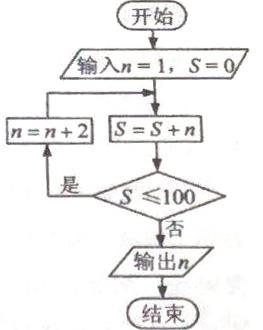
\includegraphics[width=.42\linewidth]{assets/asset-046-01.jpg}
\end{center}
\begin{choices}
  \item $17$
  \item $19$
  \item $21$
  \item $23$
\end{choices}
\begin{solution}
\textbf{答案：}$21$

\textbf{分析：}根据程序框图的算法功能可知，要计算满足 $1+3+5+\cdots+n > 100$ 的最小正奇数 $n$, 根据等差数列求和公式即可求出.

\textbf{详解：}输出的 $n$ 是满足 $1+3+5+\cdots+n > 100$ 的最小正奇数，因为 $1+3+5+\cdots+n = \frac{(1+n)\times(\frac{n-1}{2}+1)}{2} = \frac{(n+1)^2}{4} > 100$, 解得 $n > 19$, 所以输出的 $n=21$.
\end{solution}
\end{question}

\begin{question}[points=5]
\textbf{来源：}2020 年 全国I卷-文科，第 10 题\par
设 $\{a_n\}$ 是等比数列，且 $a_1 + a_2 + a_3 = 1$, $a_2 + a_3 + a_4 = 2$, 则 $a_6 + a_7 + a_8 =$
\begin{choices}
  \item $12$
  \item $24$
  \item $30$
  \item $32$
\end{choices}
\begin{solution}
\textbf{答案：}$32$

\textbf{分析：}根据已知条件求得 $q$ 的值，再由 $a_6+a_7+a_8 = q^5(a_1+a_2+a_3)$ 可求得结果.

\textbf{详解：}设等比数列 $\{a_n\}$ 的公比为 $q$, 则 $a_1+a_2+a_3 = a_1(1+q+q^2)=1$, $a_2+a_3+a_4 = a_1q(1+q+q^2)=q=2$, 因此 $a_6+a_7+a_8 = a_1q^5(1+q+q^2)=q^5=32$.
\end{solution}
\end{question}

\begin{question}[points=5]
\textbf{来源：}2020 年 全国I卷-文科，第 16 题\par
数列 $\{a_n\}$ 满足 $a_{n+2} + (-1)^n a_n = 3n - 1$, 前 $16$ 项和为 $540$, 则 $a_1 =$
\fillin[{$7$}]
\begin{solution}
\textbf{答案：}$7$

\textbf{分析：}对 $n$ 为奇偶数分类讨论，分别得出奇数项、偶数项的递推关系，由奇数项递推公式将奇数项用 $a_1$ 表示，由偶数项递推公式得出偶数项的和，建立 $a_1$ 方程，求解即可得出结论.

\textbf{详解：}由 $a_{n+2} + (-1)^n a_n = 3n - 1$, 当 $n$ 为奇数时，$a_{n+2} = a_n + 3n - 1$; 当 $n$ 为偶数时，$a_{n+2} + a_n = 3n - 1$. 设数列 $\{a_n\}$ 的前 $n$ 项和为 $S_n$, $S_{16} = a_1 + a_2 + \cdots + a_{16} = a_1 + a_3 + a_5 + \cdots + a_{15} + (a_2 + a_4) + \cdots + (a_{14} + a_{16}) = a_1 + (a_1+2) + (a_1+10) + (a_1+24) + (a_1+44) + (a_1+70) + (a_1+102) + (a_1+140) + (5+17+29+41) = 8a_1 + 392 + 92 = 8a_1 + 484 = 540$, 解得 $a_1 = 7$.
\end{solution}
\end{question}

\section*{2021 年}

\begin{question}[points=4]
\textbf{来源：}2021 年 北京卷，第 6 题\par
$\{a_n\}$ 和 $\{b_n\}$ 是两个等差数列, 其中 $\frac{a_k}{b_k}$ ($1\leq k\leq 5$) 为常值, $a_1=288$, $a_5=96$, $b_1=192$, 则 $b_3=$（ ）
\begin{choices}
  \item $64$
  \item $128$
  \item $256$
  \item $512$
\end{choices}
\begin{solution}
\textbf{答案：}B

\textbf{分析：}由已知条件求出 $b_5$ 的值, 利用等差中项的性质可求得 $b_3$ 的值.

\textbf{详解：}由已知条件可得 $\frac{a_1}{b_1}=\frac{a_5}{b_5}$, 则 $b_5=\frac{a_5 b_1}{a_1}=\frac{96\times192}{288}=64$, 因此 $b_3=\frac{b_1+b_5}{2}=\frac{192+64}{2}=128$.
\end{solution}
\end{question}

\begin{question}[points=4]
\textbf{来源：}2021 年 北京卷，第 10 题\par
数列 $\{a_n\}$ 是递增的整数数列, 且 $a_1\geq 3$, $a_1+a_2+\cdots+a_n=100$, 则 $n$ 的最大值为（ ）
\begin{choices}
  \item $9$
  \item $10$
  \item $11$
  \item $12$
\end{choices}
\begin{solution}
\textbf{答案：}C

\textbf{分析：}使数列首项、递增幅度均最小, 结合等差数列的通项及求和公式即可得解.

\textbf{详解：}若要使 $n$ 尽可能的大, 则 $a_1$, 递增幅度要尽可能小, 不妨设数列 $\{a_n\}$ 是首项为 $3$, 公差为 $1$ 的等差数列, 其前 $n$ 项和为 $S_n$, 则 $a_n=n+2$, $S_{11}=\frac{3+13}{2}\times 11=88<100$, $S_{12}=\frac{3+14}{2}\times 12=102>100$, 所以 $n$ 的最大值为 $11$.
\end{solution}
\end{question}

\begin{question}[points=15]
\textbf{来源：}2021 年 北京卷，第 21 题\par
定义 $R_p$ 数列 $\{a_n\}$: 对实数 $p$, 满足: ① $a_1+p\geq0$, $a_2+p=0$; ② $\forall n\in\mathbb{N}^*$, $a_{4n-1}<a_{4n}$; ③ $a_{m+n}\in\{a_m+a_n+p, a_m+a_n+p+1\}$, $m,n\in\mathbb{N}^*$.

(1) 对于前 $4$ 项 $2,-2,0,1$ 的数列, 可以是 $R_2$ 数列吗? 说明理由;

(2) 若 $\{a_n\}$ 是 $R_0$ 数列, 求 $a_5$ 的值;

(3) 是否存在 $p$, 使得存在 $R_p$ 数列 $\{a_n\}$, 对 $\forall n\in\mathbb{N}^*$, $S_n\geq S_{10}$? 若存在, 求出所有这样的 $p$; 若不存在, 说明理由.
\begin{solution}
\textbf{答案：}(1) 不可以, 理由见解析; (2) $a_5=1$; (3) 存在, $p=2$.

\textbf{分析：}(1) 利用性质③验证; (2) 由性质推导前四项, 再用数学归纳法; (3) 构造 $b_n=a_n+p$, 利用(2)结论.

\textbf{详解：}(1) 由性质③, $a_3\in\{a_1+a_2+2, a_1+a_2+2+1\}=\{2,3\}$, 但 $a_3=0$ 不在其中, 矛盾, 故不可以是 $R_2$ 数列.
(2) 由 $R_0$ 性质, $a_1\geq0$, $a_2=0$. 由性质③, $a_3\in\{a_1, a_1+1\}$, $a_4\in\{0,1\}$. 若 $a_4=0$, 由性质② $a_3<a_4=0$, 则 $a_1<0$ 或 $a_1+1<0$, 矛盾; 若 $a_4=1$, $a_3=a_1+1$, 由 $a_3<1$ 得 $a_1<0$, 矛盾; 故 $a_4=1$, $a_3=a_1$. 再由 $a_4=a_1+a_3$ 或 $a_4=a_1+a_3+1$, 得 $a_1=\frac{1}{2}$ 或 $0$. 若 $a_1=\frac{1}{2}$, 则 $a_2=a_{1+1}\in\{2a_1,2a_1+1\}=\{1,2\}$, 与 $a_2=0$ 矛盾. 故 $a_1=0$, 前四项为 $0,0,0,1$. 用数学归纳法证明 $a_{4n+i}=n$ ($i=1,2,3$), $a_{4n+4}=n+1$, $n\in\mathbb{N}$. 当 $n=0$ 时成立. 假设 $n\leq k$ 时成立, 则 $n=k+1$ 时, 可推出 $a_{4k+5}=k+1$, $a_{4k+6}=k+1$, $a_{4k+8}=k+2$, $a_{4k+7}=k+1$. 故 $a_5=a_{4\times1+1}=1$.
(3) 令 $b_n=a_n+p$, 则 $b_n$ 满足 $R_0$ 性质, 由(2)知 $b_{4n+i}=n$ ($i=1,2,3$), $b_{4n+4}=n+1$. 故 $a_n=b_n-p$. 要求 $S_n\geq S_{10}$ 恒成立, 即 $S_n-S_{10}\geq0$, 考察 $S_{11}-S_{10}=a_{11}=b_{11}-p=2-p\geq0$, $S_9-S_{10}=-a_{10}=-(b_{10}-p)=-(2-p)\geq0$, 故 $p=2$. 此时 $a_1,a_2,\ldots,a_{10}\leq0$, $a_j\geq0$ ($j\geq11$), 满足题意. 所以存在 $p=2$.
\end{solution}
\end{question}

\begin{question}[points=5]
\textbf{来源：}2021 年 全国甲卷-理科，第 7 题；次专题：集合与逻辑\par
等比数列 $\{a_n\}$ 的公比为 $q$，前 $n$ 项和为 $S_n$．设甲：$q>0$，乙：$\{S_n\}$ 是递增数列，则（ ）
\begin{choices}
  \item 甲是乙的充分条件但不是必要条件
  \item 甲是乙的必要条件但不是充分条件
  \item 甲是乙的充要条件
  \item 甲既不是乙的充分条件也不是乙的必要条件
\end{choices}
\begin{solution}
\textbf{答案：}B

\textbf{分析：}当 $q>0$ 时，通过举反例说明甲不是乙的充分条件；当 $\{S_n\}$ 是递增数列时，必有 $a_n>0$ 成立即可说明 $q>0$ 成立，则甲是乙的必要条件．

\textbf{详解：}当 $a_n = -2, -4, -8, \cdots$ 时，$q>0$，但 $\{S_n\}$ 递减，故甲不是乙的充分条件；若 $\{S_n\}$ 递增，则必有 $a_n>0$，进而 $q>0$，故甲是乙的必要条件．故选B．
\end{solution}
\end{question}

\begin{question}[points=12]
\textbf{来源：}2021 年 全国甲卷-理科，第 18 题\par
已知数列 $\{a_n\}$ 的各项均为正数，记 $S_n$ 为 $\{a_n\}$ 的前 $n$ 项和，从下面①②③中选取两个作为条件，证明另外一个成立．①数列 $\{a_n\}$ 是等差数列；②数列 $\{\sqrt{S_n}\}$ 是等差数列；③ $a_2 = 3a_1$．注：若选择不同的组合分别解答，则按第一个解答计分．
\begin{solution}
\textbf{答案：}答案见解析

\textbf{分析：}选①②作条件证明③时，可设 $\sqrt{S_n} = an+b$，结合 $a_n, S_n$ 的关系求出 $a_n$，利用 $\{a_n\}$ 是等差数列可证 $a_2=3a_1$；选①③作条件证明②时，根据等差数列的求和公式表示出 $S_n$，结合等差数列定义可证；选②③作条件证明①时，设出 $\sqrt{S_n}=an+b$，结合 $a_n, S_n$ 的关系求出 $a_n$，根据 $a_2=3a_1$ 可求 $b$，然后可证 $\{a_n\}$ 是等差数列．

\textbf{详解：}（1）选①②作条件证明③：设 $\sqrt{S_n}=an+b \ (a>0)$，则 $S_n = (an+b)^2$，$a_1 = (a+b)^2$，$n\ge2$ 时 $a_n = S_n - S_{n-1} = a(2an-a+2b)$．因为 $\{a_n\}$ 等差，所以 $\{a_n\}$ 通项为一次式，故 $a+b=0$？由 $a_2=3a_1$ 可推得 $b=0$，则 $a_n = a^2(2n-1)$，故 $a_2=3a_1$．（2）选①③作条件证明②：由 $a_2=3a_1$ 等差得公差 $d=2a_1$，$S_n = na_1 + \frac{n(n-1)}{2}\cdot 2a_1 = n^2 a_1$，所以 $\sqrt{S_n} = \sqrt{a_1} n$，是等差数列．（3）选②③作条件证明①：设 $\sqrt{S_n}=an+b$，同（1）得 $a_n = a(2an - a + 2b)$，由 $a_2=3a_1$ 得 $b=0$ 或 $b=-\frac{4a}{3}$，其中 $b=0$ 时 $a_n = a^2(2n-1)$ 为等差；$b=-\frac{4a}{3}$ 时 $S_1<0$ 不合题意，舍去．所以 $\{a_n\}$ 为等差数列．
\end{solution}
\end{question}

\begin{question}[points=5]
\textbf{来源：}2021 年 全国甲卷-文科，第 9 题\par
记 $S_n$ 为等比数列 $\{a_n\}$ 的前 $n$ 项和.若 $S_2=4$, $S_4=6$, 则 $S_6=$ ( )
\begin{choices}
  \item 7
  \item 8
  \item 9
  \item 10
\end{choices}
\begin{solution}
\textbf{答案：}A

\textbf{分析：}根据题目条件可得 $S_2$, $S_4-S_2$, $S_6-S_4$ 成等比数列，从而求出 $S_6-S_4=1$, 进一步求出答案.

\textbf{详解：}因为 $S_n$ 为等比数列 $\{a_n\}$ 的前 $n$ 项和，所以 $S_2$, $S_4-S_2$, $S_6-S_4$ 成等比数列. 所以 $S_2=4$, $S_4-S_2=6-4=2$, 所以 $S_6-S_4=1$, 所以 $S_6=1+S_4=1+6=7$.
\end{solution}
\end{question}

\begin{question}[points=12]
\textbf{来源：}2021 年 全国甲卷-文科，第 18 题\par
记 $S_n$ 为数列 $\{a_n\}$ 的前 $n$ 项和，已知 $a_n > 0$, $a_2 = 3a_1$, 且数列 $\{\sqrt{S_n}\}$ 是等差数列，证明：$\{a_n\}$ 是等差数列.
\begin{solution}
\textbf{答案：}证明见解析.

\textbf{分析：}先根据 $\sqrt{S_2} - \sqrt{S_1}$ 求出数列 $\{\sqrt{S_n}\}$ 的公差 $d$, 进一步写出 $\{\sqrt{S_n}\}$ 的通项，从而求出 $\{a_n\}$ 的通项公式，最终得证.

\textbf{详解：}因为数列 $\{\sqrt{S_n}\}$ 是等差数列，设公差为 $d = \sqrt{S_2} - \sqrt{S_1} = \sqrt{a_2} - \sqrt{a_1} = \sqrt{3a_1} - \sqrt{a_1} = \sqrt{a_1}(\sqrt{3}-1)$. 由 $a_2=3a_1$ 得 $d=\sqrt{a_1}(\sqrt{3}-1)$. 又 $\sqrt{S_1}=\sqrt{a_1}$, 所以 $\sqrt{S_n} = \sqrt{a_1} + (n-1)d = \sqrt{a_1} + (n-1)\sqrt{a_1}(\sqrt{3}-1) = \sqrt{a_1}((\sqrt{3}-1)n + 2-\sqrt{3})$. 则 $S_n = a_1[((\sqrt{3}-1)n + 2-\sqrt{3})^2]$. 当 $n\ge 2$ 时, $a_n = S_n - S_{n-1} = a_1[((\sqrt{3}-1)n + 2-\sqrt{3})^2 - ((\sqrt{3}-1)(n-1) + 2-\sqrt{3})^2] = a_1[2(\sqrt{3}-1)^2 n + 2(\sqrt{3}-1)(2-\sqrt{3}) - (\sqrt{3}-1)^2]$. 整理得 $a_n = 2a_1(\sqrt{3}-1)^2 n + a_1[2(\sqrt{3}-1)(2-\sqrt{3}) - (\sqrt{3}-1)^2]$. 计算可知 $a_n - a_{n-1} = 2a_1(\sqrt{3}-1)^2$ 为常数，故 $\{a_n\}$ 是等差数列.
\end{solution}
\end{question}

\begin{question}[points=12]
\textbf{来源：}2021 年 全国乙卷-理科，第 19 题\par
记$S_n$为数列$\{a_n\}$的前$n$项和，$b_n$为数列$\{S_n\}$的前$n$项积，已知$\frac{2}{S_n}+\frac{1}{b_n}=2$。

（1）证明：数列$\{b_n\}$是等差数列；

（2）求$\{a_n\}$的通项公式。
\begin{solution}
\textbf{答案：}（1）证明见解析；（2）$a_n=\begin{cases}\frac32,&n=1\\ -\frac{1}{n(n+1)},&n\geq2\end{cases}$

\textbf{详解：}（1）由已知$\frac{2}{S_n}+\frac{1}{b_n}=2$，则$\frac{b_n}{b_{n-1}}=S_n(n\geq2)$，$\Rightarrow\frac{2b_{n-1}}{b_n}+\frac{1}{b_n}=2\Rightarrow 2b_{n-1}+1=2b_n\Rightarrow b_n-b_{n-1}=\frac12(n\geq2)$，$b_1=\frac32$，故$\{b_n\}$是以$\frac32$为首项，$\frac12$为公差的等差数列。
（2）由（1）知$b_n=\frac32+(n-1)\cdot\frac12=\frac{n+2}{2}$，则$\frac{2}{S_n}+\frac{2}{n+2}=2\Rightarrow S_n=\frac{n+2}{n+1}$。$n=1$时，$a_1=S_1=\frac32$；$n\geq2$时，$a_n=S_n-S_{n-1}=\frac{n+2}{n+1}-\frac{n+1}{n}=-\frac{1}{n(n+1)}$。故$a_n=\begin{cases}\frac32,&n=1\\ -\frac{1}{n(n+1)},&n\geq2\end{cases}$。
\end{solution}
\end{question}

\begin{question}[points=12]
\textbf{来源：}2021 年 全国乙卷-文科，第 19 题\par
设 $\{a_n\}$ 是首项为1的等比数列，数列 $\{b_n\}$ 满足 $b_n = \frac{na_n}{3}$ .已知 $a_1$ ， $3a_2$ ， $9a_3$ 成等差数列.

（1）求 $\{a_n\}$ 和 $\{b_n\}$ 的通项公式；

（2）记 $S_n$ 和 $T_n$ 分别为 $\{a_n\}$ 和 $\{b_n\}$ 的前 $n$ 项和.证明：$T_n < \frac{S_n}{2}$ .
\begin{solution}
\textbf{答案：}见解析

\textbf{详解：}（1）设 $\{a_n\}$ 的公比为 $q$ ，则 $a_n = q^{n-1}$ ，
因为 $a_1, 3a_2, 9a_3$ 成等差数列，所以 $1 + 9q^2 = 2\times 3q$ ，解得 $q = \frac{1}{3}$ ，
故 $a_n = \left(\frac{1}{3}\right)^{n-1}$ ， $S_n = \frac{1-\left(\frac{1}{3}\right)^n}{1-\frac{1}{3}} = \frac{3}{2}\left(1-\frac{1}{3^n}\right)$ .
又 $b_n = \frac{n}{3^n}$ ，则 $T_n = \frac{1}{3} + \frac{2}{3^2} + \frac{3}{3^3} + \cdots + \frac{n-1}{3^{n-1}} + \frac{n}{3^n}$ ，
两边同乘 $\frac{1}{3}$ ，得 $\frac{1}{3}T_n = \frac{1}{3^2} + \frac{2}{3^3} + \frac{3}{3^4} + \cdots + \frac{n-1}{3^n} + \frac{n}{3^{n+1}}$ ，
两式相减，得 $\frac{2}{3}T_n = \frac{1}{3} + \frac{1}{3^2} + \frac{1}{3^3} + \cdots + \frac{1}{3^n} - \frac{n}{3^{n+1}}$ ，
即 $\frac{2}{3}T_n = \frac{\frac{1}{3}(1-\frac{1}{3^n})}{1-\frac{1}{3}} - \frac{n}{3^{n+1}} = \frac{1}{2}(1-\frac{1}{3^n}) - \frac{n}{3^{n+1}}$ ，
整理得 $T_n = \frac{3}{4}(1-\frac{1}{3^n}) - \frac{n}{2\cdot3^n} = \frac{3}{4} - \frac{2n+3}{4\cdot3^n}$ ，
则 $2T_n - S_n = 2\left(\frac{3}{4} - \frac{2n+3}{4\cdot3^n}\right) - \frac{3}{2}\left(1-\frac{1}{3^n}\right) = -\frac{4n+3}{2\cdot3^n} < 0$ ，
故 $T_n < \frac{S_n}{2}$ .
\end{solution}
\end{question}

\begin{question}[points=4]
\textbf{来源：}2021 年 上海春季卷，第 1 题\par
已知等差数列 $\{a_n\}$ 的首项为3，公差为2，则 $a_{10}=$  .
\fillin[{$21$}]
\begin{solution}
\textbf{答案：}$21$

\textbf{分析：}由已知结合等差数列的通项公式即可直接求解．

\textbf{详解：}因为等差数列 $\{a_n\}$ 的首项为3，公差为2，则 $a_{10}=a_1+9d=3+9\times 2=21$．
\end{solution}
\end{question}

\begin{question}[points=5]
\textbf{来源：}2021 年 上海春季卷，第 9 题\par
在无穷等比数列 $\{a_n\}$ 中，$\lim\limits_{n\to\infty}(a_1-a_n)=4$，则 $a_2$ 的取值范围是  .
\fillin[{$(-4,0)\cup(0,4)$}]
\begin{solution}
\textbf{答案：}$(-4,0)\cup(0,4)$

\textbf{分析：}由无穷等比数列的概念可得公比 $q$ 的取值范围，再由极限的运算知 $a_1=4$，从而得解．

\textbf{详解：}因为无穷等比数列 $\{a_n\}$，所以公比 $q\in(-1,0)\cup(0,1)$，则 $\lim\limits_{n\to\infty}a_n=0$，所以 $\lim\limits_{n\to\infty}(a_1-a_n)=a_1=4$，所以 $a_2=a_1q=4q\in(-4,0)\cup(0,4)$．
\end{solution}
\end{question}

\begin{question}[points=18]
\textbf{来源：}2021 年 上海春季卷，第 21 题\par
已知数列 $\{a_n\}$ 满足 $a_n\ge 0$，对任意 $n\ge 2$，$a_n$ 和 $a_{n+1}$ 中存在一项使其为另一项与 $a_{n-1}$ 的等差中项．\begin{enumerate}\item[(1)] 已知 $a_1=5$，$a_2=3$，$a_4=2$，求 $a_3$ 的所有可能取值；\item[(2)] 已知 $a_1=a_4=a_7=0$，$a_2$、$a_5$、$a_8$ 为正数，求证：$a_2$、$a_5$、$a_8$ 成等比数列，并求出公比 $q$；\item[(3)] 已知数列中恰有3项为0，即 $a_r=a_s=a_t=0$，$2<r<s<t$，且 $a_1=1$，$a_2=2$，求 $a_{r+1}+a_{s+1}+a_{t+1}$ 的最大值．\end{enumerate}
\begin{solution}
\textbf{答案：}$(1)\ a_3=1$；$(2)\ q=\frac{1}{4}$；$(3)\ \frac{21}{64}$

\textbf{分析：}（1）根据 $a_n$ 和 $a_{n+1}$ 中存在一项使其为另一项与 $a_{n-1}$ 的等差中项建立等式，然后将 $a_1$，$a_2$，$a_4$ 的值代入即可；\newline（2）根据递推关系求出 $a_5$、$a_8$，然后根据等比数列的定义进行判定即可；\newline（3）分别求出 $a_{r+1}$，$a_{s+1}$，$a_{t+1}$ 的通项公式，从而可求出各自的最大值，从而可求出所求．

\textbf{详解：}（1）由题意，$2a_n=a_{n+1}+a_{n-1}$ 或 $2a_{n+1}=a_n+a_{n-1}$，所以 $2a_2=a_3+a_1$ 解得 $a_3=1$，$2a_3=a_2+a_1$ 解得 $a_3=4$，经检验，$a_3=1$．\newline（2）证明：因为 $a_1=a_4=a_7=0$，所以 $a_3=2a_2$ 或 $a_3=\frac{a_2}{2}$，经检验，$a_3=\frac{a_2}{2}$；所以 $a_5=\frac{a_3}{2}=\frac{a_2}{4}$ 或 $a_5=-a_1=-\frac{a_2}{2}$（舍），所以 $a_5=\frac{a_2}{4}$；$a_6=\frac{a_5}{2}=\frac{a_2}{8}$ 或 $a_6=-a_5=-\frac{a_2}{4}$（舍），所以 $a_6=\frac{a_2}{8}$；$a_8=\frac{a_6}{2}=\frac{a_2}{16}$ 或 $a_8=-a_6=-\frac{a_2}{8}$（舍），所以 $a_8=\frac{a_2}{16}$；综上，$a_2$、$a_5$、$a_8$ 成等比数列，公比为 $\frac{1}{4}$．\newline（3）由 $2a_n=a_{n+1}+a_{n-1}$ 或 $2a_{n+1}=a_n+a_{n-1}$，可知 $\frac{a_{n+2}-a_{n+1}}{a_{n+1}-a_n}=1$ 或 $\frac{a_{n+2}-a_{n+1}}{a_{n+1}-a_n}=-\frac{1}{2}$，由第（2）问可知，$a_r=0$，则 $a_{r-2}=2a_{r-1}$，即 $a_{r-1}-a_{r-2}=-a_{r-1}$，所以 $a_r=0$，则 $a_{r+1}=\frac{1}{2}a_{r-1}=-\frac{1}{2}(a_{r-1}-a_{r-2})=-\frac{1}{2}\cdot(-\frac{1}{2})^i\cdot 1^{r-3-i}\cdot(a_2-a_1)=-\frac{1}{2}\cdot(-\frac{1}{2})^i$，$i\in\mathbb{N}^*$，所以 $(a_{r+1})_{\max}=\frac{1}{4}$；同理，$a_{s+1}=-\frac{1}{2}\cdot(-\frac{1}{2})^j\cdot 1^{s-2-r-j}\cdot(a_{r+1}-a_r)=-\frac{1}{2}\cdot(-\frac{1}{2})^j\cdot\frac{1}{4}$，$j\in\mathbb{N}^*$，所以 $(a_{s+1})_{\max}=\frac{1}{16}$，同理，$(a_{t+1})_{\max}=\frac{1}{64}$，所以 $a_{r+1}+a_{s+1}+a_{t+1}$ 的最大值为 $\frac{21}{64}$．
\end{solution}
\end{question}

\begin{question}[points=5]
\textbf{来源：}2021 年 上海卷，第 8 题\par
已知无穷递缩等比数列$a_1=3$, $b_n=a_{2n}$, $\{a_n\}$的各项和为9, 则数列$\{b_n\}$的各项和为．
\fillin[{$\frac{18}{5}$}]
\begin{solution}
\textbf{答案：}$\frac{18}{5}$

\textbf{分析：}利用无穷递缩等比数列求和公式建立方程求出公比，再得到$b_n$通项公式，根据特点求和.

\textbf{详解：}$S=\frac{a_1}{1-q}=\frac{3}{1-q}=9\Rightarrow q=\frac{2}{3}$，$b_n=a_{2n}=a_1\times q^{2n-1}=3\times (\frac{2}{3})^{2n-1}\Rightarrow b_1=2$, $q_0=\frac{4}{9}\Rightarrow S_b=\frac{b_1}{1-q_0}=\frac{2}{1-\frac{4}{9}}=\frac{18}{5}$
\end{solution}
\end{question}

\begin{question}[points=5]
\textbf{来源：}2021 年 上海卷，第 12 题\par
已知$a_i\in\mathbb{N}^* (i=1,2,\cdots,9)$，且对任意$k\in\mathbb{N}^* (2\le k\le 8)$都有$a_k=a_{k-1}+1$或$a_k=a_{k+1}-1$中有且仅有一个成立，$a_1=6$，$a_9=9$，则$a_1+\cdots+a_9$的最小值为．
\fillin[{$31$}]
\begin{solution}
\textbf{答案：}$31$

\textbf{分析：}注意阅读与等价转化题设中的递推关系；

\textbf{详解：}由题设，知：$a_i\ge 1$；则①$a_2=a_1+1=7$，$a_3=a_4-1$，$a_5=a_6-1$，$a_7=a_8-1$，则$a_1+a_2+\cdots+a_9=25+2(a_3+a_5+a_7)$，当$a_3=a_5=a_7=1$时，$a_1+a_2+\cdots+a_9$的和最小值为31；②$a_2=a_3-1$，$a_4=a_5-1$，$a_6=a_7-1$，$a_8=a_9-1$，则$a_1+a_2+\cdots+a_9=26+2(a_4+a_6+a_8)$，当$a_4=a_6=a_8=1$时，$a_1+a_2+\cdots+a_9$的和最小值为32；因此，$a_1+a_2+\cdots+a_9$的最小值为31
\end{solution}
\end{question}

\begin{question}[points=14]
\textbf{来源：}2021 年 上海卷，第 19 题\par
已知某企业今年（2021年）第一季度的营业额为1.1亿元，以后每个季度（一年有四个季度）营业额都比前一季度多0.05亿元，该企业第一季度利润为0.16亿元，以后每一季度的利润都比前一季度增长4%.（1）求2021第一季度起20季度的营业额总和；（2）问哪一年哪个季度的利润首次超过该季度营业额的18%？
\begin{solution}
\textbf{答案：}(1)31.5亿元；(2)2027年第二季度

\textbf{分析：}（1）根据每个季度比上个季度营业额增加0.05亿元可以知道数列为一个等差数列，求解20季度营业收入总额即为等差数列前20项的和；（2）通过数列通项公式建立数列不等式，利用计算器计算求解不等式即可。

\textbf{详解：}（1）设$a_n$为第$n$季度的营业额，$b_n$为利润，由题意得，$a_n$的首项为1.1亿元，公差为0.05亿元，所以2021到2025年，20季度营业收入总额为：$S_{20}=20a_1+\frac{20\times19}{2}\times d=31.5$（亿元）（2）由已知得，$a_n=a_1+(n-1)d=1.1+0.05(n-1)$；$b_n$的首项为0.16亿元，公比为1.04，即$b_n=b_1\cdot q^{n-1}=0.16\times1.04^{n-1}$；所以$a_n\times18\%<b_n$，利用计算器可得，$n_{\min}=26$，所以2027年第二季度该公司的利润首次超过该季度营业收入的18%
\end{solution}
\end{question}

\begin{question}[points=15]
\textbf{来源：}2021 年 天津卷，第 19 题\par
已知 $\{a_n\}$ 是公差为 $2$ 的等差数列，其前 $8$ 项和为 $64$．$\{b_n\}$ 是公比大于 $0$ 的等比数列，$b_1 = 4$，$b_3 - b_2 = 48$．

（I）求 $\{a_n\}$ 和 $\{b_n\}$ 的通项公式；

（II）记 $c_n = b_{2n} + \frac{1}{b_n}$，$n \in \mathbb{N}^*$．

（i）证明 $\{c_n^2 - c_{2n}\}$ 是等比数列；

（ii）证明 $\sum_{k=1}^n \frac{a_k a_{k+1}}{c_k^2 - c_{2k}} < 2\sqrt{2}$（$n \in \mathbb{N}^*$）．
\begin{solution}
\textbf{答案：}（I）$a_n = 2n-1$，$b_n = 4^n$；（II）证明见解析

\textbf{分析：}（I）由等差数列的求和公式运算可得 $\{a_n\}$ 的通项，由等比数列的通项公式运算可得 $\{b_n\}$ 的通项公式；
（II）（i）运算可得 $c_n^2 - c_{2n} = 2 \cdot 4^n$，结合等比数列的定义即可得证；
（ii）放缩得 $\frac{a_n a_{n+1}}{c_n^2 - c_{2n}} < \frac{4n^2}{2 \cdot 2^{2n}} = \frac{1}{2} \cdot \frac{n}{2^{n-1}}$，进而可得 $\sum_{k=1}^n \frac{a_k a_{k+1}}{c_k^2 - c_{2k}} < \frac{1}{2} \sum_{k=1}^n \frac{k}{2^{k-1}}$，结合错位相减法即可得证.

\textbf{详解：}（I）$\{a_n\}$ 公差 $d=2$，前8项和 $S_8 = 8a_1 + \frac{8\times7}{2}\times2 = 64$，得 $a_1=1$，$a_n = 2n-1$；$\{b_n\}$ 公比 $q>0$，$b_1=4$，$b_3-b_2=4q^2-4q=48$，解得 $q=4$（负舍），$b_n=4^n$；
（II）（i）$c_n = 4^{2n} + \frac{1}{4^n}$，$c_n^2 - c_{2n} = \left(4^{2n} + \frac{1}{4^n}\right)^2 - \left(4^{4n} + \frac{1}{4^{2n}}\right) = 2\cdot4^n$，$\because c_n^2 - c_{2n} \neq 0$，且 $\frac{c_{n+1}^2 - c_{2(n+1)}}{c_n^2 - c_{2n}} = \frac{2\cdot4^{n+1}}{2\cdot4^n} = 4$，$\therefore \{c_n^2 - c_{2n}\}$ 是等比数列；
（ii）$a_k a_{k+1} = (2k-1)(2k+1) = 4k^2-1 < 4k^2$，$c_k^2 - c_{2k} = 2\cdot4^k = 2\cdot2^{2k}$，$\therefore \frac{a_k a_{k+1}}{c_k^2 - c_{2k}} < \frac{4k^2}{2\cdot2^{2k}} = \frac{1}{2}\cdot\frac{k}{2^{k-1}}$，$\sum_{k=1}^n \frac{a_k a_{k+1}}{c_k^2 - c_{2k}} < \frac{1}{2} \sum_{k=1}^n \frac{k}{2^{k-1}}$，令 $T_n = \sum_{k=1}^n \frac{k}{2^{k-1}}$，则 $\frac{1}{2}T_n = \sum_{k=1}^n \frac{k}{2^k}$，两式相减得 $\frac{1}{2}T_n = 1+\frac{1}{2}+\frac{1}{2^2}+\cdots+\frac{1}{2^{n-1}} - \frac{n}{2^n} = 2\left(1-\frac{1}{2^n}\right) - \frac{n}{2^n} = 2 - \frac{n+2}{2^n}$，$T_n = 4 - \frac{n+2}{2^{n-1}}$，$\therefore \sum_{k=1}^n \frac{a_k a_{k+1}}{c_k^2 - c_{2k}} < \frac{1}{2}\left(4 - \frac{n+2}{2^{n-1}}\right) = 2 - \frac{n+2}{2^n} < 2\sqrt{2}$．
\end{solution}
\end{question}

\begin{question}[points=5]
\textbf{来源：}2021 年 新高考II卷，第 12 题\par
设正整数$n=a_0\cdot2^0+a_1\cdot2^1+\cdots+a_{k-1}\cdot2^{k-1}+a_k\cdot2^k$，其中$a_i\in\{0,1\}$，记$\omega(n)=a_0+a_1+\cdots+a_k$．则（ ）
\begin{choices}
  \item A. $\omega(2n)=\omega(n)$
  \item B. $\omega(2n+3)=\omega(n)+1$
  \item C. $\omega(8n+5)=\omega(4n+3)$
  \item D. $\omega(2^n-1)=n$
\end{choices}
\begin{solution}
\textbf{答案：}ACD

\textbf{分析：}利用$\omega(n)$的定义可判断ACD选项的正误，利用特殊值法可判断B选项的正误.

\textbf{详解：}对于A选项，$\omega(n)=a_0+a_1+\cdots+a_k$，$2n=a_0\cdot2^1+a_1\cdot2^2+\cdots+a_{k-1}\cdot2^k+a_k\cdot2^{k+1}$，所以$\omega(2n)=a_0+a_1+\cdots+a_k=\omega(n)$，A选项正确；对于B选项，取$n=2$，$2n+3=7=1\cdot2^0+1\cdot2^1+1\cdot2^2$，$\omega(7)=3$，而$2=0\cdot2^0+1\cdot2^1$，则$\omega(2)=1$，即$\omega(7)\neq\omega(2)+1$，B选项错误；对于C选项，$8n+5=a_0\cdot2^3+a_1\cdot2^4+\cdots+a_k\cdot2^{k+3}+5=1\cdot2^0+1\cdot2^2+a_0\cdot2^3+a_1\cdot2^4+\cdots+a_k\cdot2^{k+3}$，所以$\omega(8n+5)=2+a_0+a_1+\cdots+a_k$，$4n+3=a_0\cdot2^2+a_1\cdot2^3+\cdots+a_k\cdot2^{k+2}+3=1\cdot2^0+1\cdot2^1+a_0\cdot2^2+a_1\cdot2^3+\cdots+a_k\cdot2^{k+2}$，所以$\omega(4n+3)=2+a_0+a_1+\cdots+a_k$，因此$\omega(8n+5)=\omega(4n+3)$，C选项正确；对于D选项，$2^n-1=2^0+2^1+\cdots+2^{n-1}$，故$\omega(2^n-1)=n$，D选项正确.故选：ACD.
\end{solution}
\end{question}

\begin{question}[points=10]
\textbf{来源：}2021 年 新高考II卷，第 17 题\par
记$S_n$是公差不为$0$的等差数列$\{a_n\}$的前$n$项和，若$a_3=S_5$, $a_2a_4=S_4$．

（1）求数列$\{a_n\}$的通项公式$a_n$；

（2）求使$S_n>a_n$成立的$n$的最小值．
\begin{solution}
\textbf{答案：}(1) $a_n=2n-6$；(2) $7$.

\textbf{分析：}(1)由题意首先求得$a_3$的值，然后结合题意求得数列的公差即可确定数列的通项公式； (2)首先求得前$n$项和的表达式，然后求解二次不等式即可确定$n$的最小值.

\textbf{详解：}(1)由等差数列的性质可得：$S_5=5a_3$，则：$a_3=5a_3,\therefore a_3=0$，设等差数列的公差为$d$，从而有：$a_2a_4=(a_3-d)(a_3+d)=-d^2$，$S_4=a_1+a_2+a_3+a_4=(a_3-2d)+(a_3-d)+a_3+(a_3+d)=-2d$，从而：$-d^2=-2d$，由于公差不为零，故：$d=2$，数列的通项公式为：$a_n=a_3+(n-3)d=2n-6$. (2)由数列的通项公式可得：$a_1=2-6=-4$，则：$S_n=n\times(-4)+\frac{n(n-1)}{2}\times2=n^2-6n$，则不等式$S_n>a_n$即：$n^2-6n>2n-6$，整理可得：$(n-1)(n-6)>0$，解得：$n<1$或$n>6$，又$n$为正整数，故$n$的最小值为$7$.
\end{solution}
\end{question}

\begin{question}[points=5]
\textbf{来源：}2021 年 新高考I卷，第 16 题\par
某校学生在研究民间剪纸艺术时, 发现剪纸时经常会沿纸的某条对称轴把纸对折. 规格为 $20\,\text{dm} \times 12\,\text{dm}$ 的长方形纸, 对折1次共可以得到 $10\,\text{dm} \times 12\,\text{dm}$, $20\,\text{dm} \times 6\,\text{dm}$ 两种规格的图形, 它们的面积之和 $S_1 = 240\,\text{dm}^2$; 对折2次共可以得到 $5\,\text{dm} \times 12\,\text{dm}$, $10\,\text{dm} \times 6\,\text{dm}$, $20\,\text{dm} \times 3\,\text{dm}$ 三种规格的图形, 它们的面积之和 $S_2 = 180\,\text{dm}^2$; 以此类推, 则对折4次共可以得到不同规格图形的种数为; 如果对折 $n$ 次, 那么 $\sum_{k=1}^{n} S_k =$ $\text{dm}^2$.
\fillin[{$5$ ; $720 - \frac{15(n+3)}{2^{n-4}}$}]
\begin{solution}
\textbf{答案：}$5$ ; $720 - \frac{15(n+3)}{2^{n-4}}$

\textbf{分析：}列举对折4次可得规格种类数; 找出 $S_n$ 的表达式, 再利用错位相减法求和.

\textbf{详解：}对折4次可得到: $\frac{5}{4}\times12$, $\frac{5}{2}\times6$, $5\times3$, $10\times\frac{3}{2}$, $20\times\frac{3}{4}$, 共5种. $S_1=2\times120$, $S_2=3\times60$, $S_3=4\times30$, $S_4=5\times15$, 一般地 $S_n = \frac{120(n+1)}{2^{n-1}}$. 设 $S = \sum_{k=1}^n S_k = \sum_{k=1}^n \frac{120(k+1)}{2^{k-1}}$. 用错位相减法得 $S = 720 - \frac{15(n+3)}{2^{n-4}}$.
\end{solution}
\end{question}

\begin{question}[points=10]
\textbf{来源：}2021 年 新高考I卷，第 17 题\par
已知数列 $\{a_n\}$ 满足 $a_1 = 1$, $a_{n+1} = \begin{cases} a_n + 1, & n \text{为奇数}, \\ a_n + 2, & n \text{为偶数}. \end{cases}$

(1) 记 $b_n = a_{2n}$, 写出 $b_1$, $b_2$, 并求数列 $\{b_n\}$ 的通项公式;

(2) 求 $\{a_n\}$ 的前20项和.
\begin{solution}
\textbf{答案：}(1) $b_1 = 2$, $b_2 = 5$, $b_n = 3n - 1$; (2) $300$

\textbf{分析：}(1) 根据递推关系可得 $b_{n+1} = b_n + 3$, 从而可求通项. (2) 利用奇数项与偶数项的关系求和.

\textbf{详解：}(1) $b_1 = a_2 = a_1 + 1 = 2$, $b_2 = a_4 = a_3 + 1 = (a_2 + 2) + 1 = 5$. 由递推得 $a_{2k+2} = a_{2k+1} + 1$, $a_{2k+1} = a_{2k} + 2$, 故 $a_{2k+2} = a_{2k} + 3$, 即 $b_{n+1} = b_n + 3$, 所以 $\{b_n\}$ 是等差数列, $b_n = 2 + (n-1)\times 3 = 3n - 1$.
(2) $S_{20} = a_1 + a_2 + \cdots + a_{20}$. 因为 $a_1 = a_2 - 1$, $a_3 = a_4 - 1$, $\ldots$, $a_{19} = a_{20} - 1$, 所以 $S_{20} = 2(a_2 + a_4 + \cdots + a_{20}) - 10 = 2(b_1 + b_2 + \cdots + b_{10}) - 10 = 2\left(10\times 2 + \frac{9\times 10}{2}\times 3\right) - 10 = 300$.
\end{solution}
\end{question}

\begin{question}[points=4]
\textbf{来源：}2021 年 浙江卷，第 10 题\par
已知数列 $\{a_n\}$ 满足 $a_1=1$, $a_{n+1} = \frac{a_n}{1+\sqrt{a_n}}$ $(n\in\mathbb{N}^*)$. 记数列 $\{a_n\}$ 的前 $n$ 项和为 $S_n$, 则（   ）
\begin{choices}
  \item $\frac{1}{2} < S_{100} < 3$
  \item $3 < S_{100} < 4$
  \item $4 < S_{100} < \frac{9}{2}$
  \item $\frac{9}{2} < S_{100} < 5$
\end{choices}
\begin{solution}
\textbf{答案：}A

\textbf{分析：}利用倒数法得到 $\frac{1}{a_{n+1}} = \frac{1}{a_n} + \frac{1}{\sqrt{a_n}}$, 再放缩可得 $a_n$ 的范围, 进而求和.

\textbf{详解：}由 $a_{n+1} = \frac{a_n}{1+\sqrt{a_n}}$ 得 $\frac{1}{a_{n+1}} = \frac{1}{a_n} + \frac{1}{\sqrt{a_n}}$, 得 $a_n \geq \frac{4}{(n+1)^2}$, 且 $a_n \leq \frac{6}{(n+1)(n+2)}$, 求和得 $\frac{1}{2} < S_{100} < 3$.
\end{solution}
\end{question}

\begin{question}[points=15]
\textbf{来源：}2021 年 浙江卷，第 20 题\par
已知数列 $\{a_n\}$ 的前 $n$ 项和为 $S_n$, $a_1=-\frac94$, 且 $4S_{n+1}=3S_n-9$.

(1) 求数列 $\{a_n\}$ 的通项；

(2) 设数列 $\{b_n\}$ 满足 $3b_n+(n-4)a_n=0$ $(n\in\mathbb{N}^*)$, 记 $\{b_n\}$ 的前 $n$ 项和为 $T_n$, 若 $T_n \leq \lambda b_n$ 对任意 $n\in\mathbb{N}^*$ 恒成立, 求实数 $\lambda$ 的取值范围.
\begin{solution}
\textbf{答案：}(1) $a_n = -3\cdot\left(\frac34\right)^n$; (2) $[-3,1]$

\textbf{分析：}(1) 利用 $S_n$ 与 $a_n$ 的关系, 得到等比数列; (2) 先求 $b_n$, 再用错位相减法求 $T_n$, 再分离参数 $\lambda$ 求解.

\textbf{详解：}(1) 当 $n=1$ 时, $4(a_1+a_2)=3a_1-9$, 得 $a_2=-\frac{27}{16}$. 当 $n\geq2$ 时, $4S_{n+1}=3S_n-9$ 与 $4S_n=3S_{n-1}-9$ 相减得 $4a_{n+1}=3a_n$, 又 $\frac{a_2}{a_1}=\frac34$, 故 $\{a_n\}$ 是首项为 $-\frac94$, 公比为 $\frac34$ 的等比数列, 所以 $a_n = -\frac94\cdot\left(\frac34\right)^{n-1} = -3\cdot\left(\frac34\right)^n$.
(2) 由 $3b_n+(n-4)a_n=0$ 得 $b_n = (n-4)\left(\frac34\right)^n$. 则 $T_n = -3\cdot\frac34 -2\cdot\left(\frac34\right)^2 -1\cdot\left(\frac34\right)^3 +0\cdot\left(\frac34\right)^4 +\cdots+(n-4)\left(\frac34\right)^n$, 错位相减得 $T_n = -4n\left(\frac34\right)^{n+1}$. 由 $T_n\leq\lambda b_n$ 得 $-4n\left(\frac34\right)^{n+1} \leq \lambda (n-4)\left(\frac34\right)^n$, 即 $\lambda(n-4) + 3n \geq 0$ 恒成立. 当 $n=4$ 时显然成立；当 $n<4$ 时, $\lambda \leq -\frac{3n}{n-4} = -3-\frac{12}{n-4}$, 右侧最大值为1 (当 $n=3$), 故 $\lambda\leq1$；当 $n>4$ 时, $\lambda \geq -\frac{3n}{n-4} = -3-\frac{12}{n-4}$, 右侧最小值为-3 (当 $n\to\infty$), 故 $\lambda\geq-3$. 综上, $-3\leq\lambda\leq1$.
\end{solution}
\end{question}

\section*{2022 年}

\begin{question}[points=5]
\textbf{来源：}2022 年 北京卷，第 15 题\par
已知数列 $\{a_n\}$ 各项均为正数，其前 $n$ 项和 $S_n$ 满足 $a_n \cdot S_n = 9\ (n=1,2,\cdots)$。给出下列四个结论：

① $\{a_n\}$ 的第2项小于3；

② $\{a_n\}$ 为等比数列；

③ $\{a_n\}$ 为递减数列；

④ $\{a_n\}$ 中存在小于 $\dfrac{1}{100}$ 的项。

其中所有正确结论的序号是。
\fillin[{$①③④$}]
\begin{solution}
\textbf{答案：}$①③④$

\textbf{分析：}推导出 $a_n = \dfrac{9}{a_n} - \dfrac{9}{a_{n-1}}$，求出 $a_1,a_2$ 的值可判断①；利用反证法可判断②④；利用数列单调性的定义可判断③。

\textbf{详解：}由题意可知，$\forall n\in \mathbb{N}^*$，$a_n>0$，当 $n=1$ 时，$a_1^2 = 9$，得 $a_1=3$；当 $n\geq 2$ 时，由 $S_n = \dfrac{9}{a_n}$ 得 $S_{n-1} = \dfrac{9}{a_{n-1}}$，两式作差得 $a_n = \dfrac{9}{a_n} - \dfrac{9}{a_{n-1}}$，所以 $\dfrac{9}{a_{n-1}} = \dfrac{9}{a_n} - a_n$，则 $\dfrac{9}{a_2} - a_2 = 3$，整理得 $a_2^2+3a_2-9=0$，因为 $a_2>0$，解得 $a_2 = \dfrac{3\sqrt{5}-3}{2} < 3$，①对。假设数列 $\{a_n\}$ 为等比数列，设公比为 $q$，则 $a_2^2 = a_1a_3$，即 $\left(\dfrac{9}{S_2}\right)^2 = \dfrac{81}{S_1S_3}$，所以 $S_2^2 = S_1S_3$，得 $a_1^2(1+q)^2 = a_1^2(1+q+q^2)$，解得 $q=0$，不合题意，故不是等比数列，②错。当 $n\geq 2$ 时，$a_n = \dfrac{9}{a_n} - \dfrac{9}{a_{n-1}} = \dfrac{9(a_{n-1}-a_n)}{a_n a_{n-1}} > 0$，得 $a_{n-1} > a_n$，所以数列 $\{a_n\}$ 为递减数列，③对。假设对任意 $n\in \mathbb{N}^*$，$a_n \geq \dfrac{1}{100}$，则 $S_{100000} \geq 100000 \times \dfrac{1}{100} = 1000$，所以 $a_{100000} = \dfrac{9}{S_{100000}} \leq \dfrac{9}{1000} < \dfrac{1}{100}$，与假设矛盾，故④对。所以正确结论的序号是①③④。
\end{solution}
\end{question}

\begin{question}[points=15]
\textbf{来源：}2022 年 北京卷，第 21 题\par
已知 $Q: a_1, a_2, \cdots, a_k$ 为有穷整数数列。给定正整数 $m$，若对任意的 $n\in\{1,2,\cdots,m\}$，在 $Q$ 中存在 $a_i, a_{i+1}, a_{i+2}, \cdots, a_{i+j}\ (j\geq 0)$，使得 $a_i+a_{i+1}+a_{i+2}+\cdots+a_{i+j}=n$，则称 $Q$ 为 $m-$连续可表数列。

（1）判断 $Q:2,1,4$ 是否为 $5-$连续可表数列？是否为 $6-$连续可表数列？说明理由；

（2）若 $Q: a_1, a_2, \cdots, a_k$ 为 $8-$连续可表数列，求证：$k$ 的最小值为4；

（3）若 $Q: a_1, a_2, \cdots, a_k$ 为 $20-$连续可表数列，且 $a_1+a_2+\cdots+a_k<20$，求证：$k\geq 7$。
\begin{solution}
\textbf{答案：}（1）是 $5-$连续可表数列，不是 $6-$连续可表数列；（2）证明见解析；（3）证明见解析

\textbf{分析：}（1）直接利用定义验证即可；（2）先考虑 $k\leq 3$ 不符合，再列举一个 $k=4$ 合题即可；（3）$k\leq 5$ 时，根据和的个数易得显然不行，再讨论 $k=6$ 时，由 $a_1+\cdots+a_6<20$ 可知里面必然有负数，再确定负数只能是 $-1$，然后分类讨论验证不行即可。

\textbf{详解：}（1）$a_2=1$，$a_1=2$，$a_1+a_2=3$，$a_3=4$，$a_2+a_3=5$，所以 $Q$ 是 $5-$连续可表数列。不存在 $i,j$ 使得 $a_i+\cdots+a_{i+j}=6$，所以 $Q$ 不是 $6-$连续可表数列。
（2）若 $k\leq 3$，设为 $Q:a,b,c$，则至多 $a+b,b+c,a+b+c,a,b,c$ 共6个数字，没有8个，矛盾。当 $k=4$ 时，数列 $Q:1,4,1,2$ 满足 $a_1=1$，$a_4=2$，$a_3+a_4=3$，$a_2=4$，$a_1+a_2=5$，$a_1+a_2+a_3=6$，$a_2+a_3+a_4=7$，$a_1+a_2+a_3+a_4=8$，所以 $k_{\min}=4$。
（3）$Q: a_1,\cdots,a_k$，若 $i=j$ 最多有 $k$ 种，若 $i\neq j$，最多有 $C_k^2$ 种，所以最多有 $k+C_k^2 = \dfrac{k(k+1)}{2}$ 种。若 $k\leq 5$，则 $\dfrac{5\times6}{2}=15<20$，矛盾，故 $k\geq 6$。若 $k=6$，则 $\dfrac{6\times7}{2}=21$，而 $a_1+\cdots+a_6<20$，故其中必有负数。设负数为 $-m\ (m\geq 1)$，则所有数之和 $\geq m+1 + m+2 + \cdots + m+5 - m = 4m+15 \leq 19$，得 $m=1$，所以 $\{a_1,\cdots,a_6\}=\{-1,2,3,4,5,6\}$。考虑排序，排序中不能有和相同，否则不足20个。因为 $1=-1+2$（仅一种方式），所以 $-1$ 与2相邻。若 $-1$ 不在两端，则形式为 $x,-1,2,\cdots$，若 $x=6$，则 $5=6+(-1)$ 有两种方式，矛盾；同理 $x\neq 5,4,3$，故 $-1$ 在一端，不妨设为 $-1,2,A,B,C,D$。若 $A=3$，则 $5=2+3$ 有两种方式，矛盾；$A=4$ 同理；$A=5$，则 $6=-1+2+5$ 有两种方式，矛盾；故 $A=6$。由于 $7=-1+2+6$，由表法唯一知3,4不相邻，故只能为 $-1,2,6,3,5,4$ 或 $-1,2,6,4,5,3$。对于前者，$9=6+3=5+4$，矛盾；对于后者，$8=2+6=5+3$，矛盾。故 $k\neq 6$，所以 $k\geq 7$。
\end{solution}
\end{question}

\begin{question}[points=12]
\textbf{来源：}2022 年 全国甲卷-理科，第 17 题\par
记 $S_n$ 为数列 $\{a_n\}$ 的前n项和.已知 $\frac{2S_n}{n}+n=2a_n+1$.

(1) 证明：$\{a_n\}$ 是等差数列；

(2) 若 $a_4, a_7, a_9$ 成等比数列，求 $S_n$ 的最小值.
\begin{solution}
\textbf{答案：}(1) 证明见解析；(2) $-78$

\textbf{分析：}(1) 依题意可得 $2S_n+n^2=2na_n+n$，根据 $a_n=\begin{cases} S_1, & n=1 \\ S_n-S_{n-1}, & n\ge 2 \end{cases}$，作差即可得到 $a_n-a_{n-1}=1$，从而得证. (2) 由(1)及等比中项的性质求出 $a_1$，即可得到 $\{a_n\}$ 的通项公式与前n项和，再根据二次函数的性质计算可得.

\textbf{详解：}(1) 因为 $\frac{2S_n}{n}+n=2a_n+1$，即 $2S_n+n^2=2na_n+n$ ①，当 $n\ge 2$ 时，$2S_{n-1}+(n-1)^2=2(n-1)a_{n-1}+(n-1)$ ②，①-②得，$2S_n+n^2-2S_{n-1}-(n-1)^2=2na_n+n-2(n-1)a_{n-1}-(n-1)$，即 $2a_n+2n-1=2na_n-2(n-1)a_{n-1}+1$，即 $2(n-1)a_n-2(n-1)a_{n-1}=2(n-1)$，所以 $a_n-a_{n-1}=1$, $n\ge 2$ 且 $n\in\mathbb{N}^*$，所以 $\{a_n\}$ 是以1为公差的等差数列.
(2) 由(1)可得 $a_4=a_1+3$, $a_7=a_1+6$, $a_9=a_1+8$，又 $a_4, a_7, a_9$ 成等比数列，所以 $a_7^2=a_4\cdot a_9$，即 $(a_1+6)^2=(a_1+3)(a_1+8)$，解得 $a_1=-12$，所以 $a_n=n-13$，所以 $S_n=-12n+\frac{n(n-1)}{2}=\frac{1}{2}n^2-\frac{25}{2}n=\frac{1}{2}\left(n-\frac{25}{2}\right)^2-\frac{625}{8}$，所以当 $n=12$ 或 $n=13$ 时，$(S_n)_{\min}=-78$.
\end{solution}
\end{question}

\begin{question}[points=12]
\textbf{来源：}2022 年 全国甲卷-文科，第 18 题\par
记 $S_n$ 为数列 $\{a_n\}$ 的前 $n$ 项和．已知 $\frac{2S_n}{n}+n=2a_n+1$．

（1）证明：$\{a_n\}$ 是等差数列；

（2）若 $a_4, a_7, a_9$ 成等比数列，求 $S_n$ 的最小值．
\begin{solution}
\textbf{答案：}（1）证明见解析；（2）$-78$
\end{solution}
\end{question}

\begin{question}[points=5]
\textbf{来源：}2022 年 全国乙卷-理科，第 4 题\par
嫦娥二号卫星在完成探月任务后，继续进行深空探测，成为我国第一颗环绕太阳飞行的人造行星，为研究嫦娥二号绕日周期与地球绕日周期的比值，用到数列$\{b_n\}$：$b_1 = 1 + \frac{1}{\alpha_1}$，$b_2 = 1 + \frac{1}{\alpha_1 + \frac{1}{\alpha_2}}$，$b_3 = 1 + \frac{1}{\alpha_1 + \frac{1}{\alpha_2 + \frac{1}{\alpha_3}}}$，…，依此类推，其中$\alpha_k \in \mathbb{N}^* (k = 1, 2, \cdots)$．则（\qquad）
\begin{choices}
  \item $b_1 < b_5$
  \item $b_3 < b_8$
  \item $b_6 < b_2$
  \item $b_4 < b_7$
\end{choices}
\begin{solution}
\textbf{答案：}D

\textbf{分析：}根据$\alpha_k \in \mathbb{N}^* (k = 1, 2, \dots)$，再利用数列$\{b_n\}$与$\alpha_k$的关系判断$\{b_n\}$中各项的大小，即可求解.

\textbf{详解：}解：因为$\alpha_k \in \mathbb{N}^* (k = 1, 2, \cdots)$，所以$\alpha_1 < \alpha_1 + \frac{1}{\alpha_2}$，$\alpha_1 + \frac{1}{\alpha_2} > \frac{1}{\alpha_1 + \frac{1}{\alpha_2}}$，得到$b_1 > b_2$，同理$\alpha_1 + \frac{1}{\alpha_2} > \alpha_1 + \frac{1}{\alpha_2 + \frac{1}{\alpha_3}}$，可得$b_2 < b_3$，$b_1 > b_3$又因为$\frac{1}{\alpha_2} > \frac{1}{\alpha_2 + \frac{1}{\alpha_3 + \frac{1}{\alpha_4}}}$，$\alpha_1 + \frac{1}{\alpha_2 + \frac{1}{\alpha_3}} < \alpha_1 + \frac{1}{\alpha_2 + \frac{1}{\alpha_3 + \frac{1}{\alpha_4}}}$，故$b_2 < b_4$，$b_3 > b_4$；以此类推，可得$b_1 > b_3 > b_5 > b_7 > \dots$，$b_7 > b_8$，故A错误；\\$b_1 > b_7 > b_8$，故B错误；\\$\frac{1}{\alpha_2} > \frac{1}{\alpha_2 + \frac{1}{\alpha_3 + \dots \frac{1}{\alpha_6}}}$，得$b_2 < b_6$，故C错误；\\$\alpha_1 + \frac{1}{\alpha_2 + \frac{1}{\alpha_3 + \frac{1}{\alpha_4}}} > \alpha_1 + \frac{1}{\alpha_2 + \dots \frac{1}{\alpha_6 + \frac{1}{\alpha_7}}}$，得$b_4 < b_7$，故D正确.
\end{solution}
\end{question}

\begin{question}[points=5]
\textbf{来源：}2022 年 全国乙卷-理科，第 6 题\par
执行下边的程序框图，输出的$n =$（\qquad）
\begin{choices}
  \item $3$
  \item $4$
  \item $5$
  \item $6$
\end{choices}
\begin{solution}
\textbf{答案：}B

\textbf{分析：}根据框图循环计算即可.

\textbf{详解：}执行第一次循环，$b = b + 2a = 1 + 2 = 3$，\\$a = b - a = 3 - 1 = 2, n = n + 1 = 2$，\\$\frac{b^2}{a^2} - 2 = \frac{9}{4} - 2 = \frac{1}{4} > 0.01$；执行第二次循环，$b = b + 2a = 3 + 4 = 7$，\\$a = b - a = 7 - 2 = 5, n = n + 1 = 3$，\\$\frac{b^2}{a^2} - 2 = \frac{49}{25} - 2 = \frac{1}{25} > 0.01$；执行第三次循环，$b = b + 2a = 7 + 10 = 17$，\\$a = b - a = 17 - 5 = 12, n = n + 1 = 4$，\\$\frac{b^2}{a^2} - 2 = \frac{289}{144} - 2 = \frac{1}{144} < 0.01$，此时输出$n=4$.
\end{solution}
\end{question}

\begin{question}[points=5]
\textbf{来源：}2022 年 全国乙卷-理科，第 8 题\par
已知等比数列$\{a_n\}$的前3项和为168，$a_2 - a_5 = 42$，则$a_6 =$（\qquad）
\begin{choices}
  \item $14$
  \item $12$
  \item $6$
  \item $3$
\end{choices}
\begin{solution}
\textbf{答案：}D

\textbf{分析：}设等比数列$\{a_n\}$的公比为$q, q\neq0$，易得$q\neq1$，根据题意求出首项与公比，再根据等比数列的通项即可得解.

\textbf{详解：}解：设等比数列$\{a_n\}$的公比为$q, q\neq0$，若$q=1$，则$a_2-a_5=0$，与题意矛盾，所以$q\neq1$，则$\begin{cases} a_1+a_2+a_3 = \frac{a_1(1-q^3)}{1-q} = 168 \\ a_2 - a_5 = a_1q - a_1q^4 = 42 \end{cases}$，解得$\begin{cases} a_1=96 \\ q=\frac{1}{2} \end{cases}$，所以$a_6 = a_1q^5 = 3$.
\end{solution}
\end{question}

\begin{question}[points=5]
\textbf{来源：}2022 年 全国乙卷-文科，第 7 题\par
执行下边的程序框图，输出的 $n =$
\begin{choices}
  \item 3
  \item 4
  \item 5
  \item 6
\end{choices}
\begin{solution}
\textbf{答案：}B

\textbf{分析：}根据框图循环计算即可.

\textbf{详解：}执行第一次循环：$b=1+2=3$, $a=3-1=2$, $n=2$, $\left|\frac{b^2}{a^2}-2\right|=\left|\frac{9}{4}-2\right|=\frac{1}{4}>0.01$; 第二次：$b=3+4=7$, $a=7-2=5$, $n=3$, $\left|\frac{49}{25}-2\right|=\frac{1}{25}>0.01$; 第三次：$b=7+10=17$, $a=17-5=12$, $n=4$, $\left|\frac{289}{144}-2\right|=\frac{1}{144}<0.01$, 输出 $n=4$.
\end{solution}
\end{question}

\begin{question}[points=5]
\textbf{来源：}2022 年 全国乙卷-文科，第 10 题\par
已知等比数列 $\{a_n\}$ 的前3项和为168，$a_2 - a_5 = 42$, 则 $a_6 =$
\begin{choices}
  \item 14
  \item 12
  \item 6
  \item 3
\end{choices}
\begin{solution}
\textbf{答案：}D

\textbf{分析：}设等比数列的公比为 $q$, 由题意求出首项与公比，再根据通项公式即可得解.

\textbf{详解：}设公比为 $q$, 由 $a_2-a_5=42$ 得 $q\neq1$. 则 $\begin{cases} \frac{a_1(1-q^3)}{1-q}=168 \\ a_1q - a_1q^4 = 42 \end{cases}$, 解得 $a_1=96, q=\frac12$, 所以 $a_6 = a_1q^5 = 3$.
\end{solution}
\end{question}

\begin{question}[points=5]
\textbf{来源：}2022 年 全国乙卷-文科，第 13 题\par
记 $S_n$ 为等差数列 $\{a_n\}$ 的前 $n$ 项和. 若 $2S_3 = 3S_2 + 6$, 则公差 $d =$ .
\fillin[{$2$}]
\begin{solution}
\textbf{答案：}$2$

\textbf{分析：}转化条件为 $2(a_1+2d)=2a_1+d+6$, 即可得解.

\textbf{详解：}由 $2S_3=3S_2+6$ 得 $2(a_1+a_2+a_3)=3(a_1+a_2)+6$, 化简得 $2a_3=a_1+a_2+6$, 即 $2(a_1+2d)=2a_1+d+6$, 解得 $d=2$.
\end{solution}
\end{question}

\begin{question}[points=18]
\textbf{来源：}2022 年 上海卷，第 5 题\par
数列$\{a_n\}$对任意$n\in\mathbb{N}^*$且$n\geq 2$，均存在正整数$i\in[1,n-1]$，满足$a_{n+1}=2a_n-a_i$，$a_1=1$，$a_2=3$．

（1）求$a_4$可能值；

（2）命题$p$：若$a_1,a_2,\cdots,a_8$成等差数列，则$a_9<30$，证明$p$为真，同时写出$p$逆命题$q$，并判断命题$q$是真假，说明理由；

（3）若$a_{2n}=3^n$，$n\in\mathbb{N}^*$成立，求数列$\{a_n\}$的通项公式．
\begin{solution}
\textbf{答案：}（1）$a_4=7$或$9$（2）$p$真，$q$假，举例：$a_1=1,a_2=3,a_3=5,a_4=7,a_5=9,a_6=11,a_7=13,a_8=2a_7-a_5=17,a_9=2a_8-a_7=21<30$但非等差（3）$a_n=\begin{cases}1, & n=1\\5\cdot3^{\frac{n-3}{2}}, & n=2k+1,k\in\mathbb{N}^*\\3^{\frac{n}{2}}, & n=2k,k\in\mathbb{N}^*\end{cases}$

\textbf{分析：}（1）利用递推关系式可得$a_3=5$，然后计算$a_4$的值即可；（2）由题意可得$a_n=2n-1$，则$a_9=2a_8-a_i<30$，从而命题为真命题，给出反例可得命题$q$为假命题．（3）由题意可得$a_{2n+2}=2a_{2n+1}-a_i$，再利用数学归纳法证明数列单调递增，最后分类讨论即可确定数列的通项公式．

\textbf{详解：}解：（1）$a_3=2a_2-a_1=5$，$a_4=2a_3-a_2=7$或$a_4=2a_3-a_1=9$．（2）因为 $a_1,a_2,a_3,a_4,a_5,a_6,a_7,a_8$为等差数列，所以 $d=2$，$a_n=2n-1(n\in[1,8],n\in\mathbb{N}^*)$，$a_9=2a_8-a_i=30-a_i<30$．逆命题$q$：若$a_9<30$，则$a_1,a_2,a_3,a_4,a_5,a_6,a_7,a_8$为等差数列是假命题，举例：$a_1=1$，$a_2=3$，$a_3=5$，$a_4=7$，$a_5=9$，$a_6=11$，$a_7=13$，$a_8=2a_7-a_5=17$，$a_9=2a_8-a_7=21<30$但不成等差．（3）因为$a_{2n}=3^n$，所以 $a_{2n+2}=3^{n+1}$，$a_{2n+1}=2a_{2n}-a_i(i\leq 2n-1)$，$a_{2n+2}=2a_{2n+1}-a_i(i\leq 2n)$，所以 $a_{2n+2}=4a_{2n}-2a_i-a_j$，所以 $2a_i+a_j=4a_{2n}-a_{2n+2}=4\times3^n-3^{n+1}=3^n=a_{2n}$，以下用数学归纳法证明数列单调递增，即证明$a_{n+1}>a_n$恒成立：当$n=1$，$a_2>a_1$明显成立，假设$n=k$时命题成立，即$a_k>a_{k-1}>\cdots>a_2>a_1>0$，则$a_{k+1}-a_k=2a_k-a_i-a_k=a_k-a_i>0$，则$a_{k+1}>a_k$，命题得证．回到原题，分类讨论求解数列的通项公式：1．若 $i=2n-1$，则$a_{2n}=2a_{2n-1}+a_{2n-1}=3a_{2n-1}>a_{2n-1}$矛盾，2．若 $i=2n-2$，则$a_i=3^{n-1}$，所以 $a_i=3^n-2a_{2n-1}=3^{n-1}$，所以 $i=2n-2$，此时$a_{2n+1}=2a_{2n}-a_i=2\times3^n-3^{n-1}=5\times3^{n-1}$，所以 $a_n=\begin{cases}1, & n=1\\5\times3^{\frac{n-3}{2}}, & n=2k+1,k\in\mathbb{N}^*\\3^{\frac{n}{2}}, & n=2k,k\in\mathbb{N}^*\end{cases}$；3．若 $i<2n-2$，则$2a_{2n-1}<2\times3^{n-1}$，所以 $a_i=3^n-2a_{2n-1}>3^{n-1}$，所以 $i=2n-1$，所以 $a_{2n+2}=2a_{2n+1}-a_{2n-1}$（由（2）知对任意$n$成立），则$a_6=2a_5-a_3$，事实上$a_6=2a_5-a_2$矛盾．综上可得$a_n=\begin{cases}1, & n=1\\5\times3^{\frac{n-3}{2}}, & n=2k+1,k\in\mathbb{N}^*\\3^{\frac{n}{2}}, & n=2k,k\in\mathbb{N}^*\end{cases}$．
\end{solution}
\end{question}

\begin{question}[points=5]
\textbf{来源：}2022 年 上海卷，第 9 题\par
已知等差数列 $\{a_n\}$ 的公差不为零，$S_n$ 为其前$n$项和，若$S_5 = 0$，则$S_i (i = 0,1,2,\ldots,100)$ 中不同的数值有  个．
\fillin[{$98$}]
\begin{solution}
\textbf{答案：}$98$

\textbf{分析：}由等差数前$n$项和公式求出$a_1=-2d$，从而$S_n=\frac{n}{2}(n-5)d$，由此能求出结果．

\textbf{详解：}解：因为 等差数列$\{a_n\}$的公差不为零，$S_n$为其前$n$项和，$S_5=0$，所以 $5a_1+\frac{5\times4}{2}d=0$，解得$a_1=-2d$，所以 $S_n=na_1+\frac{n(n-1)}{2}d=-2nd+\frac{n(n-1)}{2}d=\frac{n}{2}(n-5)d$，因为 $d\neq0$，所以 $S_i(i=0,1,2,\ldots,100)$中$S_0=S_5=0$，$S_2=S_3=-3d$，$S_1=S_4=-2d$，其余各项均不相等，所以 $S_i(i=0,1,2,\ldots,100)$中不同的数值有：$101-3=98$．故答案为：$98$．
\end{solution}
\end{question}

\begin{question}[points=15]
\textbf{来源：}2022 年 天津卷，第 18 题\par
设 $\{a_n\}$ 是等差数列，$\{b_n\}$ 是等比数列，且 $a_1=b_1=a_2-b_2=a_3-b_3=1$．

（1）求 $\{a_n\}$ 与 $\{b_n\}$ 的通项公式；

（2）设 $\{a_n\}$ 的前 $n$ 项和为 $S_n$，求证：$(S_{n+1}+a_{n+1})b_n=S_{n+1}b_{n+1}-S_nb_n$；

（3）求 $\sum_{k=1}^{2n}[a_{k+1}-(-1)^k a_k]b_k$．
\begin{solution}
\textbf{答案：}（1）$a_n=2n-1$，$b_n=2^{n-1}$；（2）证明见解析；（3）$\frac{(3n-1)4^{n+2}+16}{9}$

\textbf{分析：}（1）利用等差等比数列的通项公式进行基本量运算；（2）由等比数列的性质及通项与前n项和的关系结合分析法即可得证；（3）先求得 $[a_{2k}-(-1)^{2k-1}a_{2k-1}]b_{2k-1}+[a_{2k+1}-(-1)^{2k}a_{2k}]b_{2k}=k\cdot4^{k+1}$，进而由并项求和可得 $T_n=\sum_{k=1}^n k\cdot4^{k+1}$，再结合错位相减法可得解.

\textbf{详解：}（1）设 $\{a_n\}$ 公差为 $d$，$\{b_n\}$ 公比为 $q$，则 $a_n=1+(n-1)d$，$b_n=q^{n-1}$，由 $a_2-b_2=a_3-b_3=1$ 得 $\begin{cases} 1+d-q=1 \\ 1+2d-q^2=1 \end{cases}$，解得 $d=q=2$（$d=q=0$ 舍去），所以 $a_n=2n-1$，$b_n=2^{n-1}$.
（2）证明：因为 $b_{n+1}=2b_n\neq0$，要证 $(S_{n+1}+a_{n+1})b_n=S_{n+1}b_{n+1}-S_nb_n$，即证 $(S_{n+1}+a_{n+1})b_n=S_{n+1}\cdot2b_n-S_nb_n$，即证 $S_{n+1}+a_{n+1}=2S_{n+1}-S_n$，即证 $a_{n+1}=S_{n+1}-S_n$，而 $a_{n+1}=S_{n+1}-S_n$ 显然成立，所以原等式成立.
（3）$[a_{2k}-(-1)^{2k-1}a_{2k-1}]b_{2k-1}+[a_{2k+1}-(-1)^{2k}a_{2k}]b_{2k}=[(4k-1)+(4k-3)]\cdot2^{2k-1}+[(4k+1)-(4k-1)]\cdot2^{2k}=k\cdot4^{k+1}$，所以 $\sum_{k=1}^{2n}[a_{k+1}-(-1)^k a_k]b_k=\sum_{k=1}^n k\cdot4^{k+1}$，记 $T_n=\sum_{k=1}^n k\cdot4^{k+1}=4^2+2\cdot4^3+3\cdot4^4+\cdots+n\cdot4^{n+1}$，则 $4T_n=4^3+2\cdot4^4+3\cdot4^5+\cdots+n\cdot4^{n+2}$，两式相减得 $-3T_n=4^2+4^3+4^4+\cdots+4^{n+1}-n\cdot4^{n+2}=\frac{4^2(1-4^n)}{1-4}-n\cdot4^{n+2}=\frac{16(4^n-1)}{3}-n\cdot4^{n+2}$，所以 $T_n=\frac{(3n-1)4^{n+2}+16}{9}$.
\end{solution}
\end{question}

\begin{question}[points=5]
\textbf{来源：}2022 年 新高考II卷，第 3 题\par
图1是中国古代建筑中的举架结构，$AA',BB',CC',DD'$是桁，相邻桁的水平距离称为步，垂直距离称为举，图2是某古代建筑屋顶截面的示意图．其中$DD_1,CC_1,BB_1,AA_1$是举，$OD_1,DC_1,CB_1,BA_1$是相等的步，相邻桁的举步之比分别为$\dfrac{DD_1}{OD_1}=0.5,\dfrac{CC_1}{DC_1}=k_1,\dfrac{BB_1}{CB_1}=k_2,\dfrac{AA_1}{BA_1}=k_3$．已知$k_1,k_2,k_3$成公差为$0.1$的等差数列，且直线$OA$的斜率为$0.725$，则$k_3=$（ ）

\begin{center}
  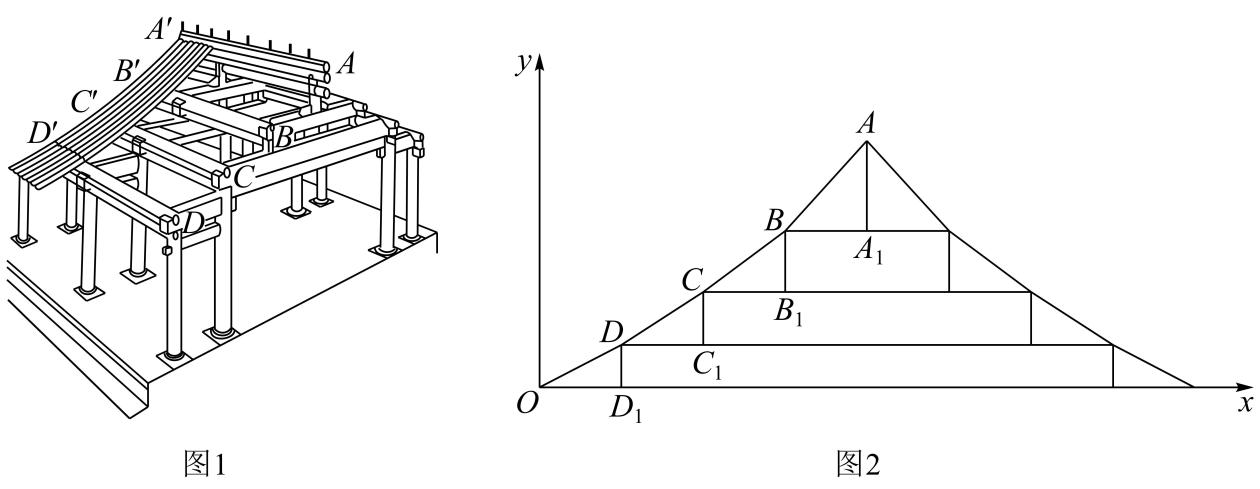
\includegraphics[width=.42\linewidth]{assets/asset-084-01.jpg}
\end{center}
\begin{choices}
  \item $0.75$
  \item $0.8$
  \item $0.85$
  \item $0.9$
\end{choices}
\begin{solution}
\textbf{答案：}$0.9$

\textbf{分析：}设$OD_1=DC_1=CB_1=BA_1=1$，则可得关于$k_3$的方程，求出其解后可得正确的选项.

\textbf{详解：}设$OD_1=DC_1=CB_1=BA_1=1$，则$CC_1=k_1,BB_1=k_2,AA_1=k_3$，依题意，有$k_3-0.2=k_1,k_3-0.1=k_2$，且$\dfrac{DD_1+CC_1+BB_1+AA_1}{OD_1+DC_1+CB_1+BA_1}=0.725$，所以$\dfrac{0.5+3k_3-0.3}{4}=0.725$，故$k_3=0.9$，故选D.
\end{solution}
\end{question}

\begin{question}[points=10]
\textbf{来源：}2022 年 新高考II卷，第 17 题\par
已知$\{a_n\}$为等差数列，$\{b_n\}$是公比为2的等比数列，且$a_2-b_2=a_3-b_3=b_4-a_4$．

(1)证明：$a_1=b_1$；

(2)求集合$\{k|b_k=a_m+a_1,1\leq m\leq 500\}$中元素个数．
\begin{solution}
\textbf{答案：}(1)证明见解析；(2)9

\textbf{分析：}(1)设数列$\{a_n\}$的公差为$d$，根据题意列出方程组即可证出；(2)根据题意化简可得$m=2^{k-2}$，即可解出.

\textbf{详解：}（1）设数列$\{a_n\}$的公差为$d$，所以$\begin{cases} a_1+d-2b_1=a_1+2d-4b_1 \\ a_1+d-2b_1=8b_1-(a_1+3d) \end{cases}$，即可解得$b_1=a_1=\dfrac{d}{2}$，所以原命题得证．
（2）由（1）知，$b_1=a_1=\dfrac{d}{2}$，所以$b_k=a_m+a_1\Leftrightarrow b_1\times 2^{k-1}=a_1+(m-1)d+a_1$，即$2^{k-1}=2m$，亦即$m=2^{k-2}\in[1,500]$，解得$2\leq k\leq 10$，所以满足等式的解$k=2,3,4,\cdots,10$，故集合$\{k|b_k=a_m+a_1,1\leq m\leq 500\}$中的元素个数为$10-2+1=9$.
\end{solution}
\end{question}

\begin{question}[points=10]
\textbf{来源：}2022 年 新高考I卷，第 17 题\par
记 $S_n$ 为数列 $\{a_n\}$ 的前 $n$ 项和, 已知 $a_1 = 1$, $\left\{\frac{S_n}{a_n}\right\}$ 是公差为 $\frac{1}{3}$ 的等差数列.

(1) 求 $\{a_n\}$ 的通项公式;

(2) 证明: $\frac{1}{a_1} + \frac{1}{a_2} + \cdots + \frac{1}{a_n} < 2$.
\begin{solution}
\textbf{答案：}(1) $a_n = \frac{n(n+1)}{2}$; (2) 见解析

\textbf{分析：}(1) 利用等差数列的通项公式求得 $\frac{S_n}{a_n} = 1 + (n-1)\cdot\frac{1}{3} = \frac{n+2}{3}$, 得到 $S_n = \frac{(n+2)a_n}{3}$, 利用和与项的关系得到当 $n \ge 2$ 时, $a_n = S_n - S_{n-1} = \frac{(n+2)a_n}{3} - \frac{(n+1)a_{n-1}}{3}$, 进而得 $\frac{a_n}{a_{n-1}} = \frac{n+1}{n-1}$, 利用累乘法求得 $a_n = \frac{n(n+1)}{2}$, 检验对于 $n=1$ 也成立. (2) 由 (1) 的结论, 利用裂项求和法得到 $\frac{1}{a_1} + \frac{1}{a_2} + \cdots + \frac{1}{a_n} = 2\left(1 - \frac{1}{n+1}\right)$, 进而证得.

\textbf{详解：}(1) $\because a_1 = 1$, $\therefore S_1 = a_1 = 1$, $\therefore \frac{S_1}{a_1} = 1$. 又 $\left\{\frac{S_n}{a_n}\right\}$ 是公差为 $\frac{1}{3}$ 的等差数列, $\therefore \frac{S_n}{a_n} = 1 + (n-1)\cdot\frac{1}{3} = \frac{n+2}{3}$, $\therefore S_n = \frac{(n+2)a_n}{3}$. $\therefore$ 当 $n \ge 2$ 时, $S_{n-1} = \frac{(n+1)a_{n-1}}{3}$, $\therefore a_n = S_n - S_{n-1} = \frac{(n+2)a_n}{3} - \frac{(n+1)a_{n-1}}{3}$, 整理得 $(n-1)a_n = (n+1)a_{n-1}$, 即 $\frac{a_n}{a_{n-1}} = \frac{n+1}{n-1}$. $\therefore a_n = a_1 \cdot \frac{a_2}{a_1} \cdot \frac{a_3}{a_2} \cdots \frac{a_{n-1}}{a_{n-2}} \cdot \frac{a_n}{a_{n-1}} = 1 \times \frac{3}{2} \times \frac{4}{3} \times \cdots \times \frac{n}{n-2} \times \frac{n+1}{n-1} = \frac{n(n+1)}{2}$. 显然对于 $n=1$ 也成立, $\therefore a_n = \frac{n(n+1)}{2}$.
(2) $\frac{1}{a_n} = \frac{2}{n(n+1)} = 2\left(\frac{1}{n} - \frac{1}{n+1}\right)$. $\therefore \frac{1}{a_1} + \frac{1}{a_2} + \cdots + \frac{1}{a_n} = 2\left[\left(1-\frac{1}{2}\right) + \left(\frac{1}{2}-\frac{1}{3}\right) + \cdots + \left(\frac{1}{n} - \frac{1}{n+1}\right)\right] = 2\left(1 - \frac{1}{n+1}\right) < 2$.
\end{solution}
\end{question}

\begin{question}[points=4]
\textbf{来源：}2022 年 浙江卷，第 10 题\par
已知数列 $\{a_n\}$ 满足 $a_1 = 1, a_{n+1} = a_n - \frac{1}{3}a_n^2$ $(n \in \mathbb{N}^*)$，则（ ）
\begin{choices}
  \item $2 < 100a_{100} < \dfrac{5}{2}$
  \item $\dfrac{5}{2} < 100a_{100} < 3$
  \item $3 < 100a_{100} < \dfrac{7}{2}$
  \item $\dfrac{7}{2} < 100a_{100} < 4$
\end{choices}
\begin{solution}
\textbf{答案：}B

\textbf{分析：}先通过递推关系式确定 $\{a_n\}$ 除去 $a_1$，其他项都在 $(0,1)$ 范围内，再利用递推公式变形得到 $\frac{1}{a_{n+1}} - \frac{1}{a_n} = \frac{1}{3-a_n} > \frac{1}{3}$，累加可求出 $\frac{1}{a_n} > \frac{1}{3}(n+2)$，得出 $100a_{100} < 3$；再利用 $\frac{1}{a_{n+1}} - \frac{1}{a_n} = \frac{1}{3-a_n} < \frac{1}{3-\frac{3}{n+2}} = \frac{1}{3}\left(1+\frac{1}{n+1}\right)$，累加可求出 $\frac{1}{a_n} - 1 < \frac{1}{3}(n-1) + \frac{1}{3}\left(\frac{1}{2}+\frac{1}{3}+\cdots+\frac{1}{n}\right)$，再次放缩可得出 $100a_{100} > \frac{5}{2}$．

\textbf{详解：}由 $a_1=1$ 易得 $a_2=\frac{2}{3} \in (0,1)$，依次类推 $a_n \in (0,1)$．由 $a_{n+1}=a_n\left(1-\frac{1}{3}a_n\right)$ 得 $\frac{1}{a_{n+1}} = \frac{3}{a_n(3-a_n)} = \frac{1}{a_n} + \frac{1}{3-a_n}$，所以 $\frac{1}{a_{n+1}} - \frac{1}{a_n} = \frac{1}{3-a_n} > \frac{1}{3}$，累加得 $\frac{1}{a_n} - 1 > \frac{1}{3}(n-1)$，即 $\frac{1}{a_n} > \frac{1}{3}(n+2)$，所以 $a_n < \frac{3}{n+2}$，$100a_{100} < \frac{100}{34} < 3$．又 $\frac{1}{a_{n+1}} - \frac{1}{a_n} = \frac{1}{3-a_n} < \frac{1}{3-\frac{3}{n+2}} = \frac{1}{3}\left(1+\frac{1}{n+1}\right)$，累加得 $\frac{1}{a_{100}} - 1 < \frac{1}{3}(99) + \frac{1}{3}\left(\frac{1}{2}+\cdots+\frac{1}{99}\right) < 33 + \frac{1}{3}\left(\frac{1}{2}\times4 + \frac{1}{6}\times94\right) < 39$，即 $\frac{1}{a_{100}} < 40$，$a_{100} > \frac{1}{40}$，所以 $100a_{100} > \frac{5}{2}$，故选B.
\end{solution}
\end{question}

\begin{question}[points=15]
\textbf{来源：}2022 年 浙江卷，第 20 题\par
已知等差数列 $\{a_n\}$ 的首项 $a_1 = -1$，公差 $d > 1$．记 $\{a_n\}$ 的前 $n$ 项和为 $S_n$ $(n \in \mathbb{N}^*)$．

（1）若 $S_4 - 2a_2 a_3 + 6 = 0$，求 $S_n$；

（2）若对于每个 $n \in \mathbb{N}^*$，存在实数 $c_n$，使 $a_n + c_n, a_{n+1} + 4c_n, a_{n+2} + 15c_n$ 成等比数列，求 $d$ 的取值范围．
\begin{solution}
\textbf{答案：}（1）$S_n = \dfrac{3n^2-5n}{2}$；（2）$1<d\le 2$

\textbf{分析：}（1）利用等差数列通项公式及前 $n$ 项和公式化简条件，求出 $d$，再求 $S_n$；（2）由等比数列定义列方程，结合一元二次方程有解的条件求 $d$ 的范围.

\textbf{详解：}（1）由 $S_4 - 2a_2a_3+6=0$，$a_1=-1$，得 $(-4+6d) - 2(-1+d)(-1+2d)+6=0$，化简得 $d^2-3d=0$，又 $d>1$，所以 $d=3$，$a_n=3n-4$，$S_n = \frac{n(a_1+a_n)}{2} = \frac{3n^2-5n}{2}$．
（2）由 $a_n+c_n, a_{n+1}+4c_n, a_{n+2}+15c_n$ 成等比数列得 $(a_{n+1}+4c_n)^2 = (a_n+c_n)(a_{n+2}+15c_n)$，代入 $a_n=-1+(n-1)d$，整理得 $c_n^2 + (14d-8nd+8)c_n + d^2 = 0$，关于 $c_n$ 的方程有实数解，判别式 $\Delta = (14d-8nd+8)^2 - 4d^2 \ge 0$ 对任意 $n\in\mathbb{N}^*$ 恒成立，即 $[(n-2)d-1][(2n-3)d-2] \ge 0$ 恒成立．当 $n=1$ 时，$(d+1)(d+2)\ge0$ 成立；当 $n=2$ 时，$(-1)(d-2)\ge0$ 得 $d\le2$；当 $n\ge3$ 时，$[(n-2)d-1][(2n-3)d-2] > (n-3)(2n-5) \ge 0$ 恒成立．又 $d>1$，所以 $1<d\le2$.
\end{solution}
\end{question}

\section*{2023 年}

\begin{question}[points=4]
\textbf{来源：}2023 年 北京卷，第 10 题\par
已知数列 $\{a_n\}$ 满足 $a_{n+1} = \dfrac{1}{4}(a_n - 6)^3 + 6\ (n = 1,2,3,\cdots)$ ，则（ ）
\begin{choices}
  \item A. 当 $a_1 = 3$ 时，$\{a_n\}$ 为递减数列，且存在常数 $M \le 0$，使得 $a_n > M$ 恒成立
  \item B. 当 $a_1 = 5$ 时，$\{a_n\}$ 为递增数列，且存在常数 $M \le 6$，使得 $a_n < M$ 恒成立
  \item C. 当 $a_1 = 7$ 时，$\{a_n\}$ 为递减数列，且存在常数 $M > 6$，使得 $a_n > M$ 恒成立
  \item D. 当 $a_1 = 9$ 时，$\{a_n\}$ 为递增数列，且存在常数 $M > 0$，使得 $a_n < M$ 恒成立
\end{choices}
\begin{solution}
\textbf{答案：}B

\textbf{分析：}法1：利用数列归纳法可判断ACD正误，利用递推可判断数列的性质，故可判断B的正误。法2：构造 $f(x)=\frac{1}{4}(x-6)^3+6-x$，利用导数求得$f(x)$的正负情况，再利用数学归纳法判断得各选项$a_n$所在区间，从而判断$\{a_n\}$的单调性；对于A，构造$h(x)=\frac{1}{4}x^3-\frac{9}{2}x^2+26x-47\ (x\le 3)$，判断得$a_{n+1}<a_n-1$，进而取$m=-[M]+4$推得$a_n>M$不恒成立；对于B，证明$a_n$所在区间同时证得后续结论；对于C，记$m_0=\log_3[2\log_{\frac{1}{4}}(M-6)+1]$，取$m=[m_0]+1$推得$a_n>M$不恒成立；对于D，构造$g(x)=\frac{1}{4}x^3-\frac{9}{2}x^2+26x-49\ (x\ge 9)$，判断得$a_{n+1}>a_n+1$，进而取$m=[M]+1$推得$a_n<M$不恒成立.

\textbf{详解：}（法1部分）因为$a_{n+1}=\frac{1}{4}(a_n-6)^3+6$，故$a_{n+1}-6=\frac{1}{4}(a_n-6)^3$。对于A，若$a_1=3$，可用数学归纳法证明$a_n\le 3$，而$a_{n+1}-a_n=\frac{1}{4}(a_n-6)^3-(a_n-6)=\frac{1}{4}(a_n-6)[(a_n-6)^2-4]$，由于$a_n-6<0$且$(a_n-6)^2-4>0$，故$a_{n+1}<a_n$，为递减数列。又$a_{n+1}-6\le \frac{9}{4}(a_n-6)$，得$6-a_{n+1}\ge 3(\frac{9}{4})^{n-1}$，故$a_{n+1}\le 6-3(\frac{9}{4})^{n-1}$，若存在$M\le 0$使得$a_n>M$恒成立，则$6-3(\frac{9}{4})^{n-1}>M$，即$n<1+\log_{\frac{9}{4}}\frac{6-M}{3}$，仅对部分$n$成立，故A不成立。对于B，若$a_1=5$，可证$5\le a_n<6$，且$a_{n+1}-a_n>0$，故为递增数列，取$M=6$满足$a_n<6$恒成立，故B正确。对于C，若$a_1=7$，可证$6<a_n\le 7$，且$a_{n+1}<a_n$，为递减数列，又$a_{n+1}-6\le \frac{1}{4}(a_n-6)$，得$a_{n+1}\le 6+(\frac{1}{4})^n$，若存在$M>6$使得$a_n>M$恒成立，则$M-6\le (\frac{1}{4})^n$，即$n\le \log_{\frac{1}{4}}(M-6)$，$n$的个数有限，矛盾，故C错误。对于D，若$a_1=9$，可证$a_n\ge 9$，且$a_{n+1}>a_n$，为递增数列，又$a_{n+1}-6>\frac{9}{4}(a_n-6)$，得$a_{n+1}\ge 6+3(\frac{9}{4})^{n-1}$，若存在$M>0$使得$a_n<M$恒成立，则$M>6+3(\frac{9}{4})^{n-1}$，即$n<\log_{\frac{9}{4}}\frac{M-6}{3}+1$，与$n$的个数有限矛盾，故D错误。故选B。
\end{solution}
\end{question}

\begin{question}[points=5]
\textbf{来源：}2023 年 北京卷，第 14 题\par
我国度量衡的发展有着悠久的历史，战国时期就已经出现了类似于砝码的、用来测量物体质量的“环权”.已知9枚环权的质量（单位：铢）从小到大构成项数为9的数列 $\{a_n\}$ ，该数列的前3项成等差数列，后7项成等比数列，且 $a_1=1, a_5=12, a_9=192$ ，则 $a_7=$ ；数列 $\{a_n\}$ 所有项的和为.
\fillin[{$48 ; 384$}]
\begin{solution}
\textbf{答案：}$48 ; 384$

\textbf{分析：}方法一：根据题意结合等差、等比数列的通项公式列式求解 $d,q$，进而可求得结果；方法二：根据等比中项求 $a_7,a_3$，再结合等差、等比数列的求和公式运算求解.

\textbf{详解：}方法一：设前3项的公差为 $d$，后7项公比为 $q>0$，则 $q^4=\frac{a_9}{a_5}=\frac{192}{12}=16$，且 $q>0$，可得 $q=2$，则 $a_3=1+2d=\frac{a_5}{q^2}=3$，即 $1+2d=3$，可得 $d=1$。空1：可得 $a_3=3, a_7=a_3q^4=48$。空2：$a_1+a_2+\cdots+a_9=1+2+3+3\times2+\cdots+3\times2^6=3+\frac{3(1-2^7)}{1-2}=384$。方法二：空1：因为 $\{a_n\}$，$3\le n\le 7$ 为等比数列，则 $a_7^2=a_5a_9=12\times192=2304$，且 $a_n>0$，所以 $a_7=48$；又因为 $a_5^2=a_3a_7$，则 $a_3=\frac{a_5^2}{a_7}=3$。空2：设后7项公比为 $q>0$，则 $q^2=\frac{a_5}{a_3}=4$，解得 $q=2$，可得 $a_1+a_2+a_3=\frac{3(a_1+a_3)}{2}=6$，$a_3+a_4+\cdots+a_9=\frac{a_3-a_9q}{1-q}=\frac{3-192\times2}{1-2}=381$，所以 $a_1+\cdots+a_9=6+381-a_3=384$。
\end{solution}
\end{question}

\begin{question}[points=15]
\textbf{来源：}2023 年 北京卷，第 21 题\par
已知数列 $\{a_n\}, \{b_n\}$ 的项数均为 $m\ (m>2)$，且 $a_n, b_n \in \{1,2,\cdots,m\}$，$\{a_n\}, \{b_n\}$ 的前 $n$ 项和分别为 $A_n, B_n$，并规定 $A_0=B_0=0$．对于 $k\in\{0,1,2,\cdots,m\}$，定义 $r_k = \max\{i\mid B_i \le A_k,\ i\in\{0,1,2,\cdots,m\}\}$，其中，$\max M$ 表示数集 $M$ 中最大的数.

（1）若 $a_1=2, a_2=1, a_3=3, b_1=1, b_2=3, b_3=3$，求 $r_0, r_1, r_2, r_3$ 的值；

（2）若 $a_1\ge b_1$，且 $2r_j \le r_{j+1} + r_{j-1},\ j=1,2,\cdots,m-1$，求 $r_n$；

（3）证明：存在 $p,q,s,t\in\{0,1,2,\cdots,m\}$，满足 $p>q,\ s>t$，使得 $A_p + B_t = A_q + B_s$．
\begin{solution}
\textbf{答案：}（1）$r_0=0, r_1=1, r_2=1, r_3=2$ （2）$r_n=n,\ n\in\mathbb{N}$ （3）证明见详解

\textbf{分析：}（1）先求 $A_0,A_1,A_2,A_3,B_0,B_1,B_2,B_3$，根据题意分析求解；（2）根据题意分析可得 $r_{i+1}-r_i\ge 1$，利用反证可得 $r_{i+1}-r_i=1$，再结合等差数列运算求解；（3）讨论 $A_m, B_m$ 的大小，根据题意结合反证法分析证明.

\textbf{详解：}（1）由题意可知：$A_0=0, A_1=2, A_2=3, A_3=6, B_0=0, B_1=1, B_2=4, B_3=7$。当 $k=0$ 时，$B_0=A_0=0$, $B_i>A_0,i=1,2,3$，故 $r_0=0$；当 $k=1$ 时，$B_0<A_1$, $B_1<A_1$, $B_i>A_1,i=2,3$，故 $r_1=1$；当 $k=2$ 时，$B_i\le A_2,i=0,1$, $B_2>A_2$, $B_3>A_2$，故 $r_2=1$；当 $k=3$ 时，$B_i\le A_3,i=0,1,2$, $B_3>A_3$，故 $r_3=2$。
（2）由题意可知：$r_n\le m$，且 $r_n\in\mathbb{N}$。因为 $a_n\ge1,b_n\ge1$，则 $A_n\ge a_1=1$, $B_n\ge b_1=1$，当且仅当 $n=1$ 时等号成立，所以 $r_0=0$, $r_1=1$。又因为 $2r_i\le r_{i-1}+r_{i+1}$，则 $r_{i+1}-r_i\ge r_i-r_{i-1}$，即 $r_m-r_{m-1}\ge r_{m-1}-r_{m-2}\ge\cdots\ge r_1-r_0=1$，可得 $r_{i+1}-r_i\ge1$。反证：假设满足 $r_{n+1}-r_n>1$ 的最小正整数为 $1\le j\le m-1$，当 $i\ge j$ 时，$r_{i+1}-r_i\ge2$；当 $i\le j-1$ 时，$r_{i+1}-r_i=1$，则 $r_m=(r_m-r_{m-1})+\cdots+(r_1-r_0)+r_0\ge2(m-j)+j=2m-j$，又因为 $1\le j\le m-1$，则 $r_m\ge2m-j\ge2m-(m-1)=m+1>m$，假设不成立，故 $r_{n+1}-r_n=1$，即数列 $\{r_n\}$ 是以首项为1，公差为1的等差数列，所以 $r_n=0+1\times n=n$，$n\in\mathbb{N}$。
（3）（ⅰ）若 $A_m\ge B_m$，构建 $S_n=A_n-B_{r_n}$，$1\le n\le m$，由题意可得：$S_n\ge0$，且 $S_n$ 为整数。反证，假设存在正整数 $K$，使得 $S_K\ge m$，则 $A_K-B_{r_K}\ge m$，$A_K-B_{r_K+1}<0$，可得 $b_{r_K+1}=B_{r_K+1}-B_{r_K}=(A_K-B_{r_K})-(A_K-B_{r_K+1})>m$，这与 $b_{r_K+1}\in\{1,2,\cdots,m\}$ 相矛盾，故对任意 $1\le n\le m,\ n\in\mathbb{N}$，均有 $S_n\le m-1$。①若存在正整数 $N$，使得 $S_N=A_N-B_{r_N}=0$，即 $A_N=B_{r_N}$，可取 $p=N,\ q=0,\ s=r_N,\ t=0$，使得 $A_p+B_t=A_q+B_s$；②若不存在正整数 $N$，使得 $S_N=0$，因为 $S_n\in\{1,2,\cdots,m-1\}$，且 $1\le n\le m$，所以必存在 $1\le X<Y\le m$，使得 $S_X=S_Y$，即 $A_X-B_{r_X}=A_Y-B_{r_Y}$，可得 $A_X+B_{r_Y}=A_Y+B_{r_X}$，可取 $p=X,\ q=Y,\ s=r_Y,\ t=r_X$，使得 $A_p+B_t=A_q+B_s$。（ⅱ）若 $A_m<B_m$，构建 $S_n=B_{r_n}-A_n$，$1\le n\le m$，由题意可得：$S_n\le0$，且 $S_n$ 为整数。反证，假设存在正整数 $K$，使得 $S_K\le -m$，则 $B_{r_K}-A_K\le -m$，$B_{r_K+1}-A_K>0$，可得 $b_{r_K+1}=B_{r_K+1}-B_{r_K}=(B_{r_K+1}-A_K)-(B_{r_K}-A_K)>m$，这与 $b_{r_K+1}\in\{1,2,\cdots,m\}$ 相矛盾，故对任意 $1\le n\le m,\ n\in\mathbb{N}$，均有 $S_n\ge 1-m$。①若存在正整数 $N$，使得 $S_N=B_{r_N}-A_N=0$，即 $A_N=B_{r_N}$，可取 $p=N,\ q=0,\ s=r_N,\ t=0$，使得 $A_p+B_t=A_q+B_s$；②若不存在正整数 $N$，使得 $S_N=0$，因为 $S_n\in\{-1,-2,\cdots,1-m\}$，且 $1\le n\le m$，所以必存在 $1\le X<Y\le m$，使得 $S_X=S_Y$，即 $B_{r_X}-A_X=B_{r_Y}-A_Y$，可得 $A_X+B_{r_Y}=A_Y+B_{r_X}$，可取 $p=X,\ q=Y,\ s=r_Y,\ t=r_X$，使得 $A_p+B_t=A_q+B_s$。综上所述：存在 $0\le p<q\le m,\ 0\le t<s\le m$ 使得 $A_p+B_t=A_q+B_s$。
\end{solution}
\end{question}

\begin{question}[points=5]
\textbf{来源：}2023 年 全国甲卷-理科，第 3 题\par
执行下面的程序框图，输出的 $B = $ （                         ）
\begin{choices}
  \item $21$
  \item $34$
  \item $55$
  \item $89$
\end{choices}
\begin{solution}
\textbf{答案：}B

\textbf{分析：}根据程序框图模拟运行，即可解出．

\textbf{详解：}当 $k = 1$ 时，判断框条件满足，第一次执行循环体，$A = 1 + 2 = 3$，$B = 3 + 2 = 5$，$k = 1 + 1 = 2$；当 $k = 2$ 时，判断框条件满足，第二次执行循环体，$A = 3 + 5 = 8$，$B = 8 + 5 = 13$，$k = 2 + 1 = 3$；当 $k = 3$ 时，判断框条件满足，第三次执行循环体，$A = 8 + 13 = 21$，$B = 21 + 13 = 34$，$k = 3 + 1 = 4$；当 $k = 4$ 时，判断框条件不满足，跳出循环体，输出 $B = 34$．
\end{solution}
\end{question}

\begin{question}[points=5]
\textbf{来源：}2023 年 全国甲卷-理科，第 5 题\par
设等比数列 $\{a_n\}$ 的各项均为正数，前 $n$ 项和为 $S_n$，若 $a_1 = 1$，$S_5 = 5S_3 - 4$，则 $S_4 = $ （                         ）
\begin{choices}
  \item $\frac{15}{8}$
  \item $\frac{65}{8}$
  \item $15$
  \item $40$
\end{choices}
\begin{solution}
\textbf{答案：}C

\textbf{分析：}根据题意列出关于 $q$ 的方程，计算出 $q$，即可求出 $S_4$．

\textbf{详解：}由题知 $1 + q + q^2 + q^3 + q^4 = 5(1 + q + q^2) - 4$，即 $q^3 + q^4 = 4q + 4q^2$，即 $q^3 + q^2 - 4q - 4 = 0$，即 $(q - 2)(q + 1)(q + 2) = 0$．由题知 $q > 0$，所以 $q = 2$．所以 $S_4 = 1 + 2 + 4 + 8 = 15$．
\end{solution}
\end{question}

\begin{question}[points=12]
\textbf{来源：}2023 年 全国甲卷-理科，第 17 题\par
设 $S_n$ 为数列 $\{a_n\}$ 的前 $n$ 项和，已知 $a_2 = 1$，$2S_n = n a_n$．

（1）求 $\{a_n\}$ 的通项公式；

（2）求数列 $\left\{ \frac{a_n+1}{2^n} \right\}$ 的前 $n$ 项和 $T_n$．
\begin{solution}
\textbf{答案：}（1）$a_n = n-1$；（2）$T_n = 2 - (2+n)\left(\frac{1}{2}\right)^n$

\textbf{分析：}（1）根据 $a_n = \begin{cases} S_1, & n=1 \\ S_n-S_{n-1}, & n\ge 2 \end{cases}$ 即可求出；（2）根据错位相减法即可解出．

\textbf{详解：}（1）因为 $2S_n = n a_n$，当 $n=1$ 时，$2a_1 = a_1$，即 $a_1=0$；当 $n=3$ 时，$2(1+a_3)=3a_3$，即 $a_3=2$；当 $n\ge2$ 时，$2S_{n-1} = (n-1)a_{n-1}$，所以 $2(S_n-S_{n-1}) = n a_n - (n-1)a_{n-1} = 2a_n$，化简得：$(n-2)a_n = (n-1)a_{n-1}$，当 $n\ge3$ 时，$\frac{a_n}{n-1} = \frac{a_{n-1}}{n-2} = \cdots = \frac{a_3}{2} = 1$，即 $a_n = n-1$，当 $n=1,2,3$ 时都满足上式，所以 $a_n = n-1 (n\in N^*)$．
（2）因为 $\frac{a_n+1}{2^n} = \frac{n}{2^n}$，所以 $T_n = 1\times\frac{1}{2} + 2\times\left(\frac{1}{2}\right)^2 + 3\times\left(\frac{1}{2}\right)^3 + \cdots + n\times\left(\frac{1}{2}\right)^n$，$\frac{1}{2}T_n = 1\times\left(\frac{1}{2}\right)^2 + 2\times\left(\frac{1}{2}\right)^3 + \cdots + (n-1)\times\left(\frac{1}{2}\right)^n + n\times\left(\frac{1}{2}\right)^{n+1}$，两式相减得，$\frac{1}{2}T_n = \frac{1}{2} + \left(\frac{1}{2}\right)^2 + \left(\frac{1}{2}\right)^3 + \cdots + \left(\frac{1}{2}\right)^n - n\times\left(\frac{1}{2}\right)^{n+1} = \frac{\frac{1}{2}\left[1-\left(\frac{1}{2}\right)^n\right]}{1-\frac{1}{2}} - n\times\left(\frac{1}{2}\right)^{n+1} = 1 - \left(1+\frac{n}{2}\right)\left(\frac{1}{2}\right)^n$，即 $T_n = 2 - (2+n)\left(\frac{1}{2}\right)^n$，$n\in N^*$．
\end{solution}
\end{question}

\begin{question}[points=5]
\textbf{来源：}2023 年 全国甲卷-文科，第 5 题\par
记 $S_n$ 为等差数列 $\{a_n\}$ 的前 $n$ 项和．若 $a_2+a_6=10, a_4a_8=45$，则 $S_5 =$（    ）
\begin{choices}
  \item $25$
  \item $22$
  \item $20$
  \item $15$
\end{choices}
\begin{solution}
\textbf{答案：}C

\textbf{分析：}方法一：根据题意直接求出等差数列 $\{a_n\}$ 的公差和首项，再根据前n项和公式即可解出；方法二：根据等差数列的性质求出等差数列 $\{a_n\}$ 的公差，再根据前n项和公式的性质即可解出．

\textbf{详解：}方法一：设等差数列 $\{a_n\}$ 的公差为 $d$，首项为 $a_1$，依题意可得，$a_2+a_6 = a_1+d+a_1+5d=10$，即 $a_1+3d=5$，又 $a_4a_8 = (a_1+3d)(a_1+7d)=45$，解得：$d=1, a_1=2$，所以 $S_5 = 5a_1+\frac{5\times4}{2}\times d = 5\times2+10=20$．故选C.
方法二：$a_2+a_6=2a_4=10$，$a_4a_8=45$，所以 $a_4=5$，$a_8=9$，从而 $d=\frac{a_8-a_4}{8-4}=1$，于是 $a_3=a_4-d=5-1=4$，所以 $S_5=5a_3=20$．故选C.
\end{solution}
\end{question}

\begin{question}[points=5]
\textbf{来源：}2023 年 全国甲卷-文科，第 6 题\par
执行下边的程序框图，则输出的 $B =$（    ）

\begin{center}
  
\includegraphics[width=.42\linewidth]{assets/asset-096-01.jpg}
\end{center}
\begin{choices}
  \item $21$
  \item $34$
  \item $55$
  \item $89$
\end{choices}
\begin{solution}
\textbf{答案：}B

\textbf{分析：}根据程序框图模拟运行即可解出．

\textbf{详解：}当 $k=1$ 时，判断框条件满足，第一次执行循环体，$A=1+2=3$，$B=3+2=5$，$k=1+1=2$；当 $k=2$ 时，判断框条件满足，第二次执行循环体，$A=3+5=8$，$B=8+5=13$，$k=2+1=3$；当 $k=3$ 时，判断框条件满足，第三次执行循环体，$A=8+13=21$，$B=21+13=34$，$k=3+1=4$；当 $k=4$ 时，判断框条件不满足，跳出循环体，输出 $B=34$．故选B.
\end{solution}
\end{question}

\begin{question}[points=5]
\textbf{来源：}2023 年 全国甲卷-文科，第 13 题\par
记 $S_n$ 为等比数列 $\{a_n\}$ 的前 $n$ 项和．若 $8S_6=7S_3$，则 $\{a_n\}$ 的公比为．
\fillin[{$-\frac{1}{2}$}]
\begin{solution}
\textbf{答案：}$-\frac{1}{2}$

\textbf{分析：}先分析 $q\neq1$，再由等比数列的前n项和公式和平方差公式化简即可求出公比 $q$.

\textbf{详解：}若 $q=1$，则由 $8S_6=7S_3$ 得 $8\cdot6a_1=7\cdot3a_1$，则 $a_1=0$，不合题意，所以 $q\neq1$．当 $q\neq1$ 时，因为 $8S_6=7S_3$，所以 $8\cdot\frac{a_1(1-q^6)}{1-q}=7\cdot\frac{a_1(1-q^3)}{1-q}$，即 $8(1-q^6)=7(1-q^3)$，即 $8(1+q^3)(1-q^3)=7(1-q^3)$，即 $8(1+q^3)=7$，解得 $q^3=-\frac{1}{8}$，所以 $q=-\frac{1}{2}$．
\end{solution}
\end{question}

\begin{question}[points=5]
\textbf{来源：}2023 年 全国乙卷-理科，第 10 题\par
已知等差数列 $\{a_n\}$ 的公差为 $\frac{2\pi}{3}$，集合 $S=\{\cos a_n|n\in\mathbb{N}^*\}$，若 $S=\{a,b\}$，则 $ab=$（ ）
\begin{choices}
  \item $-1$
  \item $-\frac{1}{2}$
  \item $0$
  \item $\frac{1}{2}$
\end{choices}
\begin{solution}
\textbf{答案：}$-\frac{1}{2}$

\textbf{分析：}根据给定的等差数列，写出通项公式，再结合余弦型函数的周期及集合只有两个元素分析、推理作答.

\textbf{详解：}依题意，等差数列 $\{a_n\}$ 中，$a_n=a_1+(n-1)\cdot\frac{2\pi}{3}=\frac{2\pi}{3}n+(a_1-\frac{2\pi}{3})$，显然函数 $y=\cos[\frac{2\pi}{3}n+(a_1-\frac{2\pi}{3})]$ 的周期为3，而 $n\in\mathbb{N}^*$，即 $\cos a_n$ 最多3个不同取值，又 $\{\cos a_n|n\in\mathbb{N}^*\}=\{a,b\}$，则在 $\cos a_1,\cos a_2,\cos a_3$ 中，$\cos a_1=\cos a_2\neq\cos a_3$ 或 $\cos a_1\neq\cos a_2=\cos a_3$，于是有 $\cos\theta=\cos(\theta+\frac{2\pi}{3})$，即有 $\theta+(\theta+\frac{2\pi}{3})=2k\pi$，$k\in\mathbb{Z}$，解得 $\theta=k\pi-\frac{\pi}{3}$，$k\in\mathbb{Z}$，所以 $ab=\cos(k\pi-\frac{\pi}{3})\cos[(k\pi-\frac{\pi}{3})+\frac{4\pi}{3}]=-\cos(k\pi-\frac{\pi}{3})\cos k\pi=-\cos^2 k\pi\cos\frac{\pi}{3}=-\frac{1}{2}$.
\end{solution}
\end{question}

\begin{question}[points=5]
\textbf{来源：}2023 年 全国乙卷-理科，第 15 题\par
已知 $\{a_n\}$ 为等比数列，$a_2a_4a_5=a_3a_6$，$a_9a_{10}=-8$，则 $a_7$=.
\fillin[{$-2$}]
\begin{solution}
\textbf{答案：}$-2$

\textbf{分析：}根据等比数列公式对 $a_2a_4a_5=a_3a_6$ 化简得 $a_1q=1$，联立 $a_9a_{10}=-8$ 求出 $q^3=-2$，最后得 $a_7=a_1q\cdot q^5=q^5=-2$.

\textbf{详解：}设 $\{a_n\}$ 的公比为 $q(q\neq0)$，则 $a_2a_4a_5=a_3a_6=a_2q\cdot a_5q$，显然 $a_n\neq0$，则 $a_4=q$，即 $a_1q^3=q$，则 $a_1q=1$，因为 $a_9a_{10}=-8$，则 $a_1q^8\cdot a_1q^9=-8$，即 $(a_1q)^2 q^{15}=-8$，则 $q^{15}=-8=(-2)^3$，则 $q^5=-2$，则 $a_7=a_1q\cdot q^5=q^5=-2$.
\end{solution}
\end{question}

\begin{question}[points=12]
\textbf{来源：}2023 年 全国乙卷-文科，第 18 题\par
记$S_n$为等差数列$\{a_n\}$的前$n$项和，已知$a_2=11, S_{10}=40$．

（1）求$\{a_n\}$的通项公式；

（2）求数列$\{|a_n|\}$的前$n$项和$T_n$．
\begin{solution}

\textbf{分析：}（1）根据题意列式求解$a_1,d$，进而可得结果；
（2）先求$S_n$，讨论$a_n$的符号去绝对值，结合$S_n$运算求解.

\textbf{详解：}（1）设等差数列的公差为$d$，由题意可得$\begin{cases}a_2=a_1+d=11\\S_{10}=10a_1+\frac{10\times9}{2}d=40\end{cases}$，即$\begin{cases}a_1+d=11\\2a_1+9d=8\end{cases}$，解得$\begin{cases}a_1=13\\d=-2\end{cases}$，所以$a_n=13-2(n-1)=15-2n$.
（2）因为$S_n=\frac{n(13+15-2n)}{2}=14n-n^2$，令$a_n=15-2n>0$，解得$n<\frac{15}{2}$，且$n\in\mathbb{N}^*$，当$n\le7$时，则$a_n>0$，可得$T_n=|a_1|+|a_2|+\cdots+|a_n|=a_1+a_2+\cdots+a_n=S_n=14n-n^2$；当$n\ge8$时，则$a_n<0$，可得$T_n=|a_1|+|a_2|+\cdots+|a_n|=(a_1+a_2+\cdots+a_7)-(a_8+\cdots+a_n)=S_7-(S_n-S_7)=2S_7-S_n=2(14\times7-7^2)-(14n-n^2)=n^2-14n+98$；综上所述：$T_n=\begin{cases}14n-n^2, & n\le7\\n^2-14n+98, & n\ge8\end{cases}$.
\end{solution}
\end{question}

\begin{question}[points=4]
\textbf{来源：}2023 年 上海卷，第 3 题\par
已知 $\{a_n\}$ 为等比数列，且 $a_1=3$，$a_3=27$，求 $a_5=$
\fillin[{$189$}]
\begin{solution}
\textbf{答案：}$189$
\end{solution}
\end{question}

\begin{question}[points=5]
\textbf{来源：}2023 年 天津卷，第 6 题\par
已知 $\{a_n\}$ 为等比数列, $S_n$ 为数列 $\{a_n\}$ 的前 $n$ 项和, $a_{n+1} = 2S_n + 2$, 则 $a_4$ 的值为 ( )
\begin{choices}
  \item 3
  \item 18
  \item 54
  \item 152
\end{choices}
\begin{solution}
\textbf{答案：}C

\textbf{分析：}对递推关系式进行赋值, 得到关于首项、公比的方程组.

\textbf{详解：}当 $n=1$ 时, $a_2 = 2a_1 + 2$, 即 $a_1 q = 2a_1 + 2$ ①. 当 $n=2$ 时, $a_3 = 2(a_1 + a_2) + 2$, 即 $a_1 q^2 = 2(a_1 + a_1 q) + 2$ ②. 联立①②得 $a_1 = 2$, $q = 3$, 则 $a_4 = a_1 q^3 = 54$.
\end{solution}
\end{question}

\begin{question}[points=15]
\textbf{来源：}2023 年 天津卷，第 19 题\par
已知 $\{a_n\}$ 是等差数列, $a_2 + a_5 = 16$, $a_5 - a_3 = 4$.

(1) 求 $\{a_n\}$ 的通项公式和 $\displaystyle\sum_{i=2^{n-1}}^{2^n-1} a_i$;

(2) 已知 $\{b_n\}$ 为等比数列, 对于任意 $k \in \mathbb{N}^*$, 若 $2^{k-1} \le n \le 2^k - 1$, 则 $b_k < a_n < b_{k+1}$,

   (Ⅰ) 当 $k \ge 2$ 时, 求证: $2^k - 1 < b_k < 2^k + 1$;

   (Ⅱ) 求 $\{b_n\}$ 的通项公式及其前 $n$ 项和.
\begin{solution}
\textbf{答案：}(1) $a_n = 2n + 1$, $\displaystyle\sum_{i=2^{n-1}}^{2^n-1} a_i = 3 \cdot 2^{2n-1}$; (2) (Ⅰ) 证明见解析; (Ⅱ) $b_n = 2^n$, 前 $n$ 项和为 $2^{n+1} - 2$

\textbf{详解：}(1) 由 $\begin{cases} a_2 + a_5 = 2a_1 + 5d = 16 \\ a_5 - a_3 = 2d = 4 \end{cases}$, 解得 $a_1 = 3$, $d = 2$, 所以 $a_n = 2n+1$. $\displaystyle\sum_{i=2^{n-1}}^{2^n-1} a_i$, 项数为 $2^n-1 - 2^{n-1} + 1 = 2^{n-1}$, 首项 $a_{2^{n-1}} = 2\cdot2^{n-1}+1 = 2^n+1$, 末项 $a_{2^n-1} = 2(2^n-1)+1 = 2^{n+1}-1$, 所以和为 $2^{n-1} \cdot \dfrac{(2^n+1)+(2^{n+1}-1)}{2} = 2^{n-1} \cdot \dfrac{3\cdot2^n}{2} = 3 \cdot 2^{2n-1}$.
(2) (Ⅰ) 由题意, 当 $2^{k-1} \le n \le 2^k-1$ 时, $b_k < a_n$. 取 $n = 2^{k-1}$, 则 $b_k < a_{2^{k-1}} = 2^k+1$. 当 $2^{k-2} \le n \le 2^{k-1}-1$ 时, $a_n < b_k$. 取 $n = 2^{k-1}-1$, 则 $a_{2^{k-1}-1} = 2(2^{k-1}-1)+1 = 2^k-1 < b_k$. 所以 $2^k-1 < b_k < 2^k+1$.
(Ⅱ) 由 (Ⅰ) 知 $1 < b_1 < 3$, $3 < b_2 < 5$, $7 < b_3 < 9$, $15 < b_4 < 17$, 猜测 $b_n = 2^n$. 若公比 $q > 2$, 则 $b_n = b_1 q^{n-1} > 2^{n-1}$, 但 $2^{n-1} > 2^n-1$ 不恒成立, 矛盾. 若公比 $q < 2$, 则 $b_n = b_1 q^{n-1} < 3 \cdot 2^{n-1}$, 但 $3\cdot2^{n-1} < 2^n+1$ 不恒成立, 矛盾. 故 $q=2$, $b_1 = 2$, 所以 $b_n = 2^n$. 前 $n$ 项和 $S_n = \dfrac{2(1-2^n)}{1-2} = 2^{n+1} - 2$.
\end{solution}
\end{question}

\begin{question}[points=5]
\textbf{来源：}2023 年 新高考II卷，第 8 题\par
记$S_{n}$为等比数列$\{a_{n}\}$的前$n$项和，若$S_{4}=-5$，$S_{6}=21S_{2}$，则$S_{8}=$（ \quad ）
\begin{choices}
  \item A. $120$
  \item B. $85$
  \item C. $-85$
  \item D. $-120$
\end{choices}
\begin{solution}
\textbf{答案：}C

\textbf{分析：}方法一：根据等比数列的前$n$项和公式求出公比，再根据$S_{4},S_{8}$的关系即可解出；方法二：根据等比数列的前$n$项和的性质求解.

\textbf{详解：}方法一：设等比数列$\{a_{n}\}$的公比为$q$，首项为$a_{1}$，若$q=1$则$S_{6}=6a_{1}=3\times2a_{1}=3S_{2}$，与题意不符，所以$q\neq1$；由$S_{4}=-5$，$S_{6}=21S_{2}$可得$\dfrac{a_{1}(1-q^{4})}{1-q}=-5$，$\dfrac{a_{1}(1-q^{6})}{1-q}=21\times\dfrac{a_{1}(1-q^{2})}{1-q}$，由后式可得$1+q^{2}+q^{4}=21$，解得$q^{2}=4$，所以$S_{8}=\dfrac{a_{1}(1-q^{8})}{1-q}=\dfrac{a_{1}(1-q^{4})}{1-q}\times(1+q^{4})=-5\times(1+16)=-85$.
方法二：设等比数列$\{a_{n}\}$的公比为$q$，因为$S_{4}=-5$，$S_{6}=21S_{2}$，所以$q\neq-1$，从而$S_{2},S_{4}-S_{2},S_{6}-S_{4},S_{8}-S_{6}$成等比数列，所以有$(-5-S_{2})^{2}=S_{2}(21S_{2}+5)$，解得$S_{2}=-1$或$S_{2}=\dfrac{5}{4}$；当$S_{2}=-1$时，$S_{2},S_{4}-S_{2},S_{6}-S_{4},S_{8}-S_{6}$即为$-1,-4,-16,S_{8}+21$，易知$S_{8}+21=-64$，即$S_{8}=-85$；当$S_{2}=\dfrac{5}{4}$时，$S_{4}=a_{1}+a_{2}+a_{3}+a_{4}=(a_{1}+a_{2})(1+q^{2})=S_{2}(1+q^{2})>0$，与$S_{4}=-5$矛盾，舍去.
\end{solution}
\end{question}

\begin{question}[points=10]
\textbf{来源：}2023 年 新高考II卷，第 18 题\par
$\{a_{n}\}$为等差数列，$b_{n}=\begin{cases}a_{n}-6, & n\text{为奇数}\\ 2a_{n}, & n\text{为偶数}\end{cases}$，记$S_{n}$，$T_{n}$分别为数列$\{a_{n}\}$，$\{b_{n}\}$的前$n$项和，$S_{4}=32$，$T_{3}=16$．

（1）求$\{a_{n}\}$的通项公式；

（2）证明：当$n>5$时，$T_{n}>S_{n}$．
\begin{solution}
\textbf{答案：}（1）$a_{n}=2n+3$；（2）证明见解析.

\textbf{分析：}（1）设等差数列$\{a_{n}\}$的公差为$d$，用$a_{1},d$表示$S_{n}$及$T_{n}$，即可求解作答.
（2）方法1，利用（1）的结论求出$S_{n}$，$b_{n}$，再分奇偶结合分组求和法求出$T_{n}$，并与$S_{n}$作差比较作答；方法2，利用（1）的结论求出$S_{n}$，$b_{n}$，再分奇偶借助等差数列前$n$项和公式求出$T_{n}$，并与$S_{n}$作差比较作答.

\textbf{详解：}（1）设等差数列$\{a_{n}\}$的公差为$d$，而$b_{n}=\begin{cases}a_{n}-6, & n=2k-1\\ 2a_{n}, & n=2k\end{cases}$，$k\in\mathbb{N}^{*}$，则$b_{1}=a_{1}-6$，$b_{2}=2a_{2}=2a_{1}+2d$，$b_{3}=a_{3}-6=a_{1}+2d-6$，于是$\begin{cases}S_{4}=4a_{1}+6d=32\\ T_{3}=4a_{1}+4d-12=16\end{cases}$，解得$a_{1}=5$，$d=2$，$a_{n}=a_{1}+(n-1)d=2n+3$，所以数列$\{a_{n}\}$的通项公式是$a_{n}=2n+3$.
（2）方法1：由（1）知，$S_{n}=\dfrac{n(5+2n+3)}{2}=n^{2}+4n$，$b_{n}=\begin{cases}2n-3, & n=2k-1\\ 4n+6, & n=2k\end{cases}$，$k\in\mathbb{N}^{*}$，当$n$为偶数时，$b_{n-1}+b_{n}=2(n-1)-3+4n+6=6n+1$，$T_{n}=\dfrac{13+(6n+1)}{2}\cdot\dfrac{n}{2}=\dfrac{3}{2}n^{2}+\dfrac{7}{2}n$，当$n>5$时，$T_{n}-S_{n}=\left(\dfrac{3}{2}n^{2}+\dfrac{7}{2}n\right)-(n^{2}+4n)=\dfrac{1}{2}n(n-1)>0$，因此$T_{n}>S_{n}$；当$n$为奇数时，$T_{n}=T_{n+1}-b_{n+1}=\dfrac{3}{2}(n+1)^{2}+\dfrac{7}{2}(n+1)-[4(n+1)+6]=\dfrac{3}{2}n^{2}+\dfrac{5}{2}n-5$，当$n>5$时，$T_{n}-S_{n}=\left(\dfrac{3}{2}n^{2}+\dfrac{5}{2}n-5\right)-(n^{2}+4n)=\dfrac{1}{2}(n+2)(n-5)>0$，因此$T_{n}>S_{n}$，所以当$n>5$时，$T_{n}>S_{n}$.
方法2：由（1）知，$S_{n}=n^{2}+4n$，$b_{n}=\begin{cases}2n-3, & n=2k-1\\ 4n+6, & n=2k\end{cases}$，$k\in\mathbb{N}^{*}$，当$n$为偶数时，$T_{n}=(b_{1}+b_{3}+\cdots+b_{n-1})+(b_{2}+b_{4}+\cdots+b_{n})=\dfrac{-1+2(n-1)-3}{2}\cdot\dfrac{n}{2}+\dfrac{14+4n+6}{2}\cdot\dfrac{n}{2}=\dfrac{3}{2}n^{2}+\dfrac{7}{2}n$，当$n>5$时，$T_{n}-S_{n}=\dfrac{1}{2}n(n-1)>0$，因此$T_{n}>S_{n}$；当$n$为奇数时，若$n\ge3$，则$T_{n}=(b_{1}+b_{3}+\cdots+b_{n})+(b_{2}+b_{4}+\cdots+b_{n-1})=\dfrac{-1+2n-3}{2}\cdot\dfrac{n+1}{2}+\dfrac{14+4(n-1)+6}{2}\cdot\dfrac{n-1}{2}=\dfrac{3}{2}n^{2}+\dfrac{5}{2}n-5$，显然$T_{1}=b_{1}=-1$满足上式，因此当$n$为奇数时，$T_{n}=\dfrac{3}{2}n^{2}+\dfrac{5}{2}n-5$，当$n>5$时，$T_{n}-S_{n}=\dfrac{1}{2}(n+2)(n-5)>0$，因此$T_{n}>S_{n}$，所以当$n>5$时，$T_{n}>S_{n}$.
\end{solution}
\end{question}

\begin{question}[points=12]
\textbf{来源：}2023 年 新高考I卷，第 20 题\par
设等差数列 $\{a_n\}$ 的公差为 $d$，且 $d>1$．令 $b_n=\frac{n^2+n}{a_n}$，记 $S_n, T_n$ 分别为数列 $\{a_n\}, \{b_n\}$ 的前 $n$ 项和．

（1）若 $3a_2=3a_1+a_3, S_3+T_3=21$，求 $\{a_n\}$ 的通项公式；

（2）若 $\{b_n\}$ 为等差数列，且 $S_{99}-T_{99}=99$，求 $d$．
\begin{solution}
\textbf{答案：}（1）$a_n=3n$；（2）$d=\frac{51}{50}$

\textbf{分析：}（1）根据等差数列的通项公式建立方程求解即可；（2）由 $\{b_n\}$ 为等差数列得出 $a_1=d$ 或 $a_1=2d$，再由等差数列的性质可得 $a_{50}-b_{50}=1$，分类讨论即可得解。

\textbf{详解：}（1）因为 $3a_2=3a_1+a_3$，所以 $3d=a_1+2d$，解得 $a_1=d$，所以 $S_3=3a_2=3(a_1+d)=6d$，又 $T_3=b_1+b_2+b_3=\frac{2}{d}+\frac{6}{2d}+\frac{12}{3d}=\frac{9}{d}$，所以 $S_3+T_3=6d+\frac{9}{d}=21$，即 $2d^2-7d+3=0$，解得 $d=3$ 或 $d=\frac{1}{2}$（舍去），所以 $a_n=a_1+(n-1)\cdot d=3n$。（2）因为 $\{b_n\}$ 为等差数列，所以 $2b_2=b_1+b_3$，即 $\frac{12}{a_2}=\frac{2}{a_1}+\frac{12}{a_3}$，所以 $6(\frac{1}{a_2}-\frac{1}{a_3})=\frac{6d}{a_2a_3}=\frac{1}{a_1}$，即 $a_1^2-3a_1d+2d^2=0$，解得 $a_1=d$ 或 $a_1=2d$，因为 $d>1$，所以 $a_n>0$，又 $S_{99}-T_{99}=99$，由等差数列性质知，$99a_{50}-99b_{50}=99$，即 $a_{50}-b_{50}=1$，所以 $a_{50}-\frac{2550}{a_{50}}=1$，即 $a_{50}^2-a_{50}-2550=0$，解得 $a_{50}=51$ 或 $a_{50}=-50$（舍去）。当 $a_1=2d$ 时，$a_{50}=a_1+49d=51d=51$，解得 $d=1$，与 $d>1$ 矛盾，无解；当 $a_1=d$ 时，$a_{50}=a_1+49d=50d=51$，解得 $d=\frac{51}{50}$。综上，$d=\frac{51}{50}$。
\end{solution}
\end{question}

\section*{2024 年}

\begin{question}[points=5]
\textbf{来源：}2024 年 北京卷，第 14 题；次专题：立体几何\par
已知三个圆柱的体积为公比为10的等比数列。第一个圆柱的直径为65mm，第二、三个圆柱的直径为325mm，第三个圆柱的高为230mm，求前两个圆柱的高度分别为。
\fillin[{$\dfrac{115}{2}\text{mm},23\text{mm}$}]
\begin{solution}
\textbf{答案：}$\dfrac{115}{2}\text{mm},23\text{mm}$

\textbf{分析：}根据体积为公比为10的等比数列可得关于高度的方程组，求出其解后可得前两个圆柱的高度。

\textbf{详解：}设第一个圆柱的高为 $h_1$，第二个圆柱的高为 $h_2$，则 $\dfrac{\pi\left(\dfrac{325}{2}\right)^2 h_2}{\pi\left(\dfrac{65}{2}\right)^2 h_1} = 10$，$\dfrac{\pi\left(\dfrac{325}{2}\right)^2 \times 230}{\pi\left(\dfrac{325}{2}\right)^2 h_2} = 10$，故 $h_2 = 23\text{mm}$，$h_1 = \dfrac{115}{2}\text{mm}$。
\end{solution}
\end{question}

\begin{question}[points=5]
\textbf{来源：}2024 年 北京卷，第 15 题\par
已知 $M = \{k \mid a_k = b_k\}$，$a_n$，$b_n$ 不为常数列且各项均不相同，下列正确的是。

① $a_n$，$b_n$ 均为等差数列，则 $M$ 中最多一个元素；

② $a_n$，$b_n$ 均为等比数列，则 $M$ 中最多三个元素；

③ $a_n$ 为等差数列，$b_n$ 为等比数列，则 $M$ 中最多三个元素；

④ $a_n$ 单调递增，$b_n$ 单调递减，则 $M$ 中最多一个元素。
\fillin[{$①③④$}]
\begin{solution}
\textbf{答案：}$①③④$

\textbf{分析：}利用两类数列的散点图的特征可判断①④的正误，利用反例可判断②的正误，结合通项公式的特征及反证法可判断③的正误。

\textbf{详解：}对于①，因为 $\{a_n\}, \{b_n\}$ 均为等差数列，故它们的散点图分布在直线上，而两条直线至多有一个公共点，故 $M$ 中至多一个元素，故①正确。
对于②，取 $a_n = 2^{n-1}$，$b_n = -(-2)^{n-1}$，则 $\{a_n\}, \{b_n\}$ 均为等比数列，但当 $n$ 为偶数时，有 $a_n = 2^{n-1} = b_n = -(-2)^{n-1}$，此时 $M$ 中有无穷多个元素，故②错误。
对于③，设 $b_n = Aq^n$（$Aq \neq 0, q \neq \pm 1$），$a_n = kn + b$（$k \neq 0$）。若 $M$ 中至少四个元素，则关于 $n$ 的方程 $Aq^n = kn + b$ 至少有4个不同的正数解。若 $q>0, q\neq 1$，则由 $y=Aq^n$ 和 $y=kn+b$ 的散点图可得关于 $n$ 的方程 $Aq^n = kn+b$ 至多有两个不同的解，矛盾；若 $q<0, q\neq \pm 1$，考虑关于 $n$ 的方程 $Aq^n = kn+b$ 奇数解的个数和偶数解的个数。当 $Aq^n = kn+b$ 有偶数解，此方程即为 $A|q|^n = kn+b$，方程至多有两个偶数解，且有两个偶数解时 $Ak\ln|q|>0$，否则 $Ak\ln|q|<0$，因 $y=A|q|^n, y=kn+b$ 单调性相反，方程 $A|q|^n = kn+b$ 至多一个偶数解。当 $Aq^n = kn+b$ 有奇数解，此方程即为 $-A|q|^n = kn+b$，方程至多有两个奇数解，且有两个奇数解时 $-Ak\ln|q|>0$ 即 $Ak\ln|q|<0$，否则 $Ak\ln|q|>0$，因 $y=-A|q|^n, y=kn+b$ 单调性相反，方程 $-A|q|^n = kn+b$ 至多一个奇数解。因为 $Ak\ln|q|>0$，$Ak\ln|q|<0$ 不可能同时成立，故 $Aq^n = kn+b$ 不可能有4个不同的正数解，故③正确。
对于④，因为 $\{a_n\}$ 为单调递增，$\{b_n\}$ 为递减数列，前者散点图呈上升趋势，后者的散点图呈下降趋势，两者至多一个交点，故④正确。
故答案为：①③④。
\end{solution}
\end{question}

\begin{question}[points=14]
\textbf{来源：}2024 年 北京卷，第 21 题；次专题：集合与逻辑\par
设集合 $M = \{(i,j,s,t) \mid i\in\{1,2\}, j\in\{3,4\}, s\in\{5,6\}, t\in\{7,8\}, 2|(i+j+s+t)\}$。对于给定有穷数列 $A:\{a_n\}(1\leq n\leq 8)$，及序列 $\Omega:\omega_1,\omega_2,\dots,\omega_s$，$\omega_k=(i_k,j_k,s_k,t_k)\in M$，定义变换 $T$：将数列 $A$ 的第 $i_1,j_1,s_1,t_1$ 项加1，得到数列 $T_1(A)$；将数列 $T_1(A)$ 的第 $i_2,j_2,s_2,t_2$ 项加1，得到数列 $T_2T_1(A)$；重复上述操作，得到数列 $T_s\cdots T_2T_1(A)$，记为 $\Omega(A)$。

（1）给定数列 $A:1,3,2,4,6,3,1,9$ 和序列 $\Omega:(1,3,5,7),(2,4,6,8),(1,3,5,7)$，写出 $\Omega(A)$；

（2）是否存在序列 $\Omega$，使得 $\Omega(A)$ 为 $a_1+2, a_2+6, a_3+4, a_4+2, a_5+8, a_6+2, a_7+4, a_8+4$，若存在，写出一个符合条件的 $\Omega$；若不存在，请说明理由；

（3）若数列 $A$ 的各项均为正整数，且 $a_1+a_3+a_5+a_7$ 为偶数，证明：“存在序列 $\Omega$，使得 $\Omega(A)$ 为常数列”的充要条件为“$a_1+a_2=a_3+a_4=a_5+a_6=a_7+a_8$”。
\begin{solution}
\textbf{答案：}（1）$\Omega(A):3,4,4,5,8,4,3,10$；（2）不存在，理由见解析；（3）证明见解析

\textbf{分析：}（1）直接按照 $\Omega(A)$ 的定义写出 $\Omega(A)$ 即可；（2）利用反证法，假设存在符合条件的 $\Omega$，由此列出方程组，进一步说明方程组无解即可；（3）分充分性和必要性两方面论证。

\textbf{详解：}（1）$\Omega(A):3,4,4,5,8,4,3,10$。
（2）假设存在符合条件的 $\Omega$，可知 $\Omega(A)$ 的第1,2项之和为 $a_1+a_2+s$，第3,4项之和为 $a_3+a_4+s$，则 $\begin{cases} (a_1+2)+(a_2+6)=a_1+a_2+s \ (a_3+4)+(a_4+2)=a_3+a_4+s \end{cases}$，而该方程组无解，故假设不成立，故不存在符合条件的 $\Omega$。
（3）设序列 $T_k\cdots T_2T_1(A)$ 为 $\{a_{k,n}\}(1\leq n\leq 8)$，特别规定 $a_{0,n}=a_n(1\leq n\leq 8)$。
必要性：若存在序列 $\Omega:\omega_1,\omega_2,\dots,\omega_s$，使得 $\Omega(A)$ 为常数列，则 $a_{s,1}=a_{s,2}=a_{s,3}=a_{s,4}=a_{s,5}=a_{s,6}=a_{s,7}=a_{s,8}$，所以 $a_{s,1}+a_{s,2}=a_{s,3}+a_{s,4}=a_{s,5}+a_{s,6}=a_{s,7}+a_{s,8}$。根据 $T_k\cdots T_2T_1(A)$ 的定义，显然有 $a_{k,2j-1}+a_{k,2j}=a_{k-1,2j-1}+a_{k-1,2j}$，这里 $j=1,2,3,4$，$k=1,2,\dots$。所以不断使用该式就得到 $a_1+a_2=a_3+a_4=a_5+a_6=a_7+a_8$，必要性得证。
充分性：若 $a_1+a_2=a_3+a_4=a_5+a_6=a_7+a_8$。由已知 $a_1+a_3+a_5+a_7$ 为偶数，而 $a_1+a_2=a_3+a_4=a_5+a_6=a_7+a_8$，所以 $a_2+a_4+a_6+a_8=4(a_1+a_2)-(a_1+a_3+a_5+a_7)$ 也是偶数。我们设 $T_s\cdots T_2T_1(A)$ 是通过合法的序列 $\Omega$ 的变换能得到的所有可能的数列 $\Omega(A)$ 中，使得 $a_{s,1}-a_{s,2}+a_{s,3}-a_{s,4}+a_{s,5}-a_{s,6}+a_{s,7}-a_{s,8}$ 最小的一个。上面已经证明 $a_{k,2j-1}+a_{k,2j}=a_{k-1,2j-1}+a_{k-1,2j}$，这里 $j=1,2,3,4$，$k=1,2,\dots$。从而由 $a_1+a_2=a_3+a_4=a_5+a_6=a_7+a_8$ 可得 $a_{s,1}+a_{s,2}=a_{s,3}+a_{s,4}=a_{s,5}+a_{s,6}=a_{s,7}+a_{s,8}$。同时，由于 $i_k+j_k+s_k+t_k$ 总是偶数，所以 $a_{k,1}+a_{k,3}+a_{k,5}+a_{k,7}$ 和 $a_{k,2}+a_{k,4}+a_{k,6}+a_{k,8}$ 的奇偶性保持不变，从而 $a_{s,1}+a_{s,3}+a_{s,5}+a_{s,7}$ 和 $a_{s,2}+a_{s,4}+a_{s,6}+a_{s,8}$ 都是偶数。
下面证明不存在 $j=1,2,3,4$ 使得 $a_{s,2j-1}-a_{s,2j}\geq 2$。假设存在，根据对称性，不妨设 $j=1$，$a_{s,2j-1}-a_{s,2j}\geq 2$，即 $a_{s,1}-a_{s,2}\geq 2$。
情况1：若 $a_{s,3}-a_{s,4}+a_{s,5}-a_{s,6}+a_{s,7}-a_{s,8}=0$，则由 $a_{s,1}+a_{s,3}+a_{s,5}+a_{s,7}$ 和 $a_{s,2}+a_{s,4}+a_{s,6}+a_{s,8}$ 都是偶数，知 $a_{s,1}-a_{s,2}\geq 4$。对该数列连续作四次变换 $(2,3,5,8)$，$(2,4,6,8)$，$(2,3,6,7)$，$(2,4,5,7)$ 后，新的 $a_{s+4,1}-a_{s+4,2}+a_{s+4,3}-a_{s+4,4}+a_{s+4,5}-a_{s+4,6}+a_{s+4,7}-a_{s+4,8}$ 相比原来的 $a_{s,1}-a_{s,2}+a_{s,3}-a_{s,4}+a_{s,5}-a_{s,6}+a_{s,7}-a_{s,8}$ 减少4，这与 $a_{s,1}-a_{s,2}+a_{s,3}-a_{s,4}+a_{s,5}-a_{s,6}+a_{s,7}-a_{s,8}$ 的最小性矛盾。
情况2：若 $a_{s,3}-a_{s,4}+a_{s,5}-a_{s,6}+a_{s,7}-a_{s,8}>0$，不妨设 $a_{s,3}-a_{s,4}>0$。
情况2-1：如果 $a_{s,3}-a_{s,4}\geq 1$，则对该数列连续作两次变换 $(2,4,5,7)$，$(2,4,6,8)$ 后，新的 $a_{s+2,1}-a_{s+2,2}+a_{s+2,3}-a_{s+2,4}+a_{s+2,5}-a_{s+2,6}+a_{s+2,7}-a_{s+2,8}$ 相比原来的 $a_{s,1}-a_{s,2}+a_{s,3}-a_{s,4}+a_{s,5}-a_{s,6}+a_{s,7}-a_{s,8}$ 至少减少2，这与最小性矛盾。
情况2-2：如果 $a_{s,4}-a_{s,3}\geq 1$，则对该数列连续作两次变换 $(2,3,5,8)$，$(2,3,6,7)$ 后，新的 $a_{s+2,1}-a_{s+2,2}+a_{s+2,3}-a_{s+2,4}+a_{s+2,5}-a_{s+2,6}+a_{s+2,7}-a_{s+2,8}$ 相比原来的至少减少2，这与最小性矛盾。
这就说明无论如何都会导致矛盾，所以对任意的 $j=1,2,3,4$ 都有 $a_{s,2j-1}-a_{s,2j}\leq 1$。
假设存在 $j=1,2,3,4$ 使得 $a_{s,2j-1}-a_{s,2j}=1$，则 $a_{s,2j-1}+a_{s,2j}$ 是奇数，所以 $a_{s,1}+a_{s,2}=a_{s,3}+a_{s,4}=a_{s,5}+a_{s,6}=a_{s,7}+a_{s,8}$ 都是奇数，设为 $2N+1$。则此时对任意 $j=1,2,3,4$，由 $|a_{s,2j-1}-a_{s,2j}|\leq 1$ 可知必有 $\{a_{s,2j-1},a_{s,2j}\}=\{N,N+1\}$。而 $a_{s,1}+a_{s,3}+a_{s,5}+a_{s,7}$ 和 $a_{s,2}+a_{s,4}+a_{s,6}+a_{s,8}$ 都是偶数，故集合 $\{m|a_{s,m}=N\}$ 中的四个元素 $i,j,s,t$ 之和为偶数，对该数列进行一次变换 $(i,j,s,t)$，则该数列成为常数列，新的 $a_{s+1,1}-a_{s+1,2}+a_{s+1,3}-a_{s+1,4}+a_{s+1,5}-a_{s+1,6}+a_{s+1,7}-a_{s+1,8}$ 等于零，比原来的 $a_{s,1}-a_{s,2}+a_{s,3}-a_{s,4}+a_{s,5}-a_{s,6}+a_{s,7}-a_{s,8}$ 更小，这与最小性矛盾。
综上，只可能 $a_{s,2j-1}-a_{s,2j}=0$（$j=1,2,3,4$），而 $a_{s,1}+a_{s,2}=a_{s,3}+a_{s,4}=a_{s,5}+a_{s,6}=a_{s,7}+a_{s,8}$，故 $\{a_{s,n}\}=\Omega(A)$ 是常数列，充分性得证。
\end{solution}
\end{question}

\begin{question}[points=5]
\textbf{来源：}2024 年 全国甲卷-理科，第 4 题\par
等差数列 $\{a_n\}$ 的前 $n$ 项和为 $S_n$，若 $S_5=S_{10}$，$a_5=1$，则 $a_1=$ （   ）
\begin{choices}
  \item $-2$
  \item $\dfrac{7}{3}$
  \item $1$
  \item $2$
\end{choices}
\begin{solution}
\textbf{答案：}B

\textbf{分析：}由 $S_5=S_{10}$ 结合等差中项的性质可得 $a_8=0$，即可计算出公差，即可得 $a_1$ 的值。

\textbf{详解：}由 $S_{10}-S_5=a_6+a_7+a_8+a_9+a_{10}=5a_8=0$，则 $a_8=0$，则等差数列 $\{a_n\}$ 的公差 $d=\frac{a_8-a_5}{3}=-\frac{1}{3}$，故 $a_1=a_5-4d=1-4\times\left(-\frac{1}{3}\right)=\frac{7}{3}$。
\end{solution}
\end{question}

\begin{question}[points=12]
\textbf{来源：}2024 年 全国甲卷-理科，第 18 题\par
记 $S_n$ 为数列 $\{a_n\}$ 的前 $n$ 项和，且 $4S_n=3a_n+4$。

（1）求 $\{a_n\}$ 的通项公式；

（2）设 $b_n=(-1)^{n-1}na_n$，求数列 $\{b_n\}$ 的前 $n$ 项和 $T_n$。
\begin{solution}
\textbf{答案：}（1）$a_n=4\cdot(-3)^{n-1}$；（2）$T_n=(2n-1)\cdot3^n+1$

\textbf{分析：}（1）利用退位法可求 $\{a_n\}$ 的通项公式；（2）利用错位相减法可求 $T_n$。

\textbf{详解：}（1）当 $n=1$ 时，$4S_1=4a_1=3a_1+4$，解得 $a_1=4$。当 $n\ge2$ 时，$4S_{n-1}=3a_{n-1}+4$，所以 $4S_n-4S_{n-1}=4a_n=3a_n-3a_{n-1}$ 即 $a_n=-3a_{n-1}$，而 $a_1=4\neq0$，故 $a_n\neq0$，故 $\frac{a_n}{a_{n-1}}=-3$，所以数列 $\{a_n\}$ 是以4为首项，$-3$ 为公比的等比数列，所以 $a_n=4\cdot(-3)^{n-1}$。
（2）$b_n=(-1)^{n-1}\cdot n\cdot4\cdot(-3)^{n-1}=4n\cdot3^{n-1}$，所以 $T_n=b_1+b_2+b_3+\cdots+b_n=4\cdot3^0+8\cdot3^1+12\cdot3^2+\cdots+4n\cdot3^{n-1}$，故 $3T_n=4\cdot3^1+8\cdot3^2+12\cdot3^3+\cdots+4n\cdot3^n$，所以 $-2T_n=4+4\cdot3^1+4\cdot3^2+\cdots+4\cdot3^{n-1}-4n\cdot3^n=4+4\cdot\frac{3(1-3^{n-1})}{1-3}-4n\cdot3^n=4+2\cdot3\cdot(3^{n-1}-1)-4n\cdot3^n=(2-4n)\cdot3^n-2$，$\therefore T_n=(2n-1)\cdot3^n+1$。
\end{solution}
\end{question}

\begin{question}[points=5]
\textbf{来源：}2024 年 全国甲卷-文科，第 4 题\par
等差数列 $\{a_n\}$ 的前 $n$ 项和为 $S_n$，若 $S_9 = 1$，则 $a_3 + a_7 =$（ ）
\begin{choices}
  \item $-2$
  \item $\frac{7}{3}$
  \item $1$
  \item $\frac{2}{9}$
\end{choices}
\begin{solution}
\textbf{答案：}D

\textbf{分析：}可以根据等差数列的基本量，即将题目条件全转化成 $a_1$ 和 $d$ 来处理，亦可用等差数列的性质进行处理，或者特殊值法处理.

\textbf{详解：}方法一：利用等差数列的基本量：由 $S_9 = 1$，根据等差数列的求和公式，$S_9 = 9a_1 + \frac{9 \times 8}{2}d = 1 \iff 9a_1 + 36d = 1$，又 $a_3 + a_7 = a_1 + 2d + a_1 + 6d = 2a_1 + 8d = \frac{2}{9}(9a_1 + 36d) = \frac{2}{9}$．方法二：利用等差数列的性质：根据等差数列的性质，$a_1 + a_9 = a_3 + a_7$，由 $S_9 = 1$，根据等差数列的求和公式，$S_9 = \frac{9(a_1 + a_9)}{2} = \frac{9(a_3 + a_7)}{2} = 1$，故 $a_3 + a_7 = \frac{2}{9}$．方法三：特殊值法：不妨取等差数列公差 $d = 0$，则 $S_9 = 1 = 9a_1 \Rightarrow a_1 = \frac{1}{9}$，则 $a_3 + a_7 = 2a_1 = \frac{2}{9}$.
\end{solution}
\end{question}

\begin{question}[points=12]
\textbf{来源：}2024 年 全国甲卷-文科，第 15 题\par
已知等比数列 $\{a_n\}$ 的前 $n$ 项和为 $S_n$，且 $2S_n = 3a_{n+1} - 3$．

（1）求 $\{a_n\}$ 的通项公式；

（2）求数列 $\{S_n\}$ 的通项公式．
\begin{solution}
\textbf{答案：}（1）$a_n = \left(\frac{5}{3}\right)^{n-1}$；（2）$S_n = \frac{3}{2}\left(\frac{5}{3}\right)^n - \frac{3}{2}$

\textbf{分析：}（1）利用退位法可求公比，再求出首项后可求通项；（2）利用等比数列的求和公式可求 $S_n$.

\textbf{详解：}（1）因为 $2S_n = 3a_{n+1} - 3$，故 $2S_{n-1} = 3a_n - 3$，所以 $2a_n = 3a_{n+1} - 3a_n\ (n \ge 2)$，即 $5a_n = 3a_{n+1}$，故等比数列的公比为 $q = \frac{5}{3}$，又 $2a_1 = 3a_2 - 3 = 3a_1 \times \frac{5}{3} - 3 = 5a_1 - 3$，故 $a_1 = 1$，故 $a_n = \left(\frac{5}{3}\right)^{n-1}$．
（2）由等比数列求和公式得 $S_n = \frac{1 \times \left[1 - \left(\frac{5}{3}\right)^n\right]}{1 - \frac{5}{3}} = \frac{3}{2}\left(\frac{5}{3}\right)^n - \frac{3}{2}$.
\end{solution}
\end{question}

\begin{question}[points=5]
\textbf{来源：}2024 年 上海卷，第 12 题\par
无穷等比数列$\{a_n\}$满足首项$a_1>0$，$q>1$，记$I_n=\{x-y\mid x,y\in[a_1,a_2]\cup[a_n,a_{n+1}]\}$，若对任意正整数$n$集合$I_n$是闭区间，则$q$的取值范围是.
\fillin[{$q\ge2$}]
\begin{solution}
\textbf{答案：}$q\ge2$

\textbf{分析：}当$n\ge2$时，不妨设$x\ge y$，则$x-y\in[0,a_2-a_1]\cup[a_n-a_2,a_{n+1}-a_1]\cup[0,a_{n+1}-a_n]$，结合$I_n$为闭区间可得$q-2\ge-\frac{1}{q^{n-2}}$对任意的$n\ge2$恒成立，故可求$q$的取值范围.

\textbf{详解：}由题设有$a_n=a_1q^{n-1}$，因为$a_1>0,q>1$，故$a_{n+1}>a_n$，故$[a_n,a_{n+1}]=[a_1q^{n-1},a_1q^n]$，当$n=1$时，$x,y\in[a_1,a_2]$，故$x-y\in[a_1-a_2,a_2-a_1]$，此时$I_1$为闭区间，当$n\ge2$时，不妨设$x\ge y$，若$x,y\in[a_1,a_2]$，则$x-y\in[0,a_2-a_1]$，若$y\in[a_1,a_2],x\in[a_n,a_{n+1}]$，则$x-y\in[a_n-a_2,a_{n+1}-a_1]$，若$x,y\in[a_n,a_{n+1}]$，则$x-y\in[0,a_{n+1}-a_n]$，综上，$x-y\in[0,a_2-a_1]\cup[a_n-a_2,a_{n+1}-a_1]\cup[0,a_{n+1}-a_n]$，又$I_n$为闭区间等价于$[0,a_2-a_1]\cup[a_n-a_2,a_{n+1}-a_1]\cup[0,a_{n+1}-a_n]$为闭区间，而$a_{n+1}-a_1>a_{n+1}-a_n>a_2-a_1$，故$a_{n+1}-a_n\ge a_n-a_2$对任意$n\ge2$恒成立，故$a_{n+1}-2a_n+a_2\ge0$即$a_1q^{n-1}(q-2)+a_2\ge0$，故$q^{n-2}(q-2)+1\ge0$，故$q-2\ge-\frac{1}{q^{n-2}}$对任意的$n\ge2$恒成立，因$q>1$，故当$n\to+\infty$时，$-\frac{1}{q^{n-2}}\to0$，故$q-2\ge0$即$q\ge2$．故答案为：$q\ge2$.
\end{solution}
\end{question}

\begin{question}[points=15]
\textbf{来源：}2024 年 天津卷，第 19 题\par
已知数列 $\{a_n\}$ 是公比大于 $0$ 的等比数列. 其前 $n$ 项和为 $S_n$. 若 $a_1=1$, $S_2=a_3-1$.

(1) 求数列 $\{a_n\}$ 前 $n$ 项和 $S_n$;

(2) 设 $b_n=\begin{cases} k, & n=a_k \\ b_{n-1}+2k, & a_k<n<a_{k+1} \end{cases}$, $b_1=1$, 其中 $k$ 是大于 $1$ 的正整数.

(i) 当 $n=a_{k+1}$ 时, 求证: $b_{n-1}\geq a_k\cdot b_n$;

(ii) 求 $\sum_{i=1}^{S_n} b_i$.
\begin{solution}
\textbf{答案：}(1) $S_n=2^n-1$; (2) (i) 证明见解析; (ii) $\sum_{i=1}^{S_n} b_i = \frac{(3n-1)4^n+1}{9}$

\textbf{分析：}(1) 设公比为 $q$, 利用 $S_2=a_3-1$ 求出 $q$, 再求和公式. (2) (i) 由 $a_k=2^{k-1}$, $n=2^k$, 推导 $b_{n-1}$ 和 $b_n$, 利用作差法证明不等式. (ii) 分段求和, 利用等差数列求和公式和裂项相消法.

\textbf{详解：}(1) 设等比数列 $\{a_n\}$ 的公比为 $q>0$, 由 $a_1=1$, $S_2=a_3-1$ 得 $1+q=q^2-1$, 即 $q^2-q-2=0$, 解得 $q=2$ (舍负). 所以 $a_n=2^{n-1}$, $S_n=\frac{1-2^n}{1-2}=2^n-1$.
(2) (i) 由 (1) 知 $a_k=2^{k-1}$, $a_{k+1}=2^k$. 当 $n=a_{k+1}=2^k$ 时, $a_k< n-1 < a_{k+1}$, 故 $b_n=b_{2^k}=k+1$, 而 $b_{n-1}=b_{2^k-1}=b_{a_k}+(2^k-1-2^{k-1})\cdot 2k = k + (2^{k-1}-1)\cdot 2k = k + 2^k k - 2k = k(2^k-1)$. 所以 $b_{n-1}-a_kb_n = k(2^k-1) - 2^{k-1}(k+1) = 2^{k-1}k - k - 2^{k-1} = 2^{k-1}(k-1) - k \geq 2(k-1)-k = k-2 \geq 0$ (当且仅当 $k=2$ 等号成立). 故 $b_{n-1}\geq a_k b_n$.
(ii) 由 $S_n=2^n-1$. 求和时, 考虑分段. 当 $2^{k-1}\leq i \leq 2^k-1$ 时, $b_i$ 构成等差数列, 首项 $b_{2^{k-1}}=k$, 公差 $2k$, 项数 $2^{k-1}$. 则 $\sum_{i=2^{k-1}}^{2^k-1} b_i = k\cdot 2^{k-1} + \frac{2^{k-1}(2^{k-1}-1)}{2}\cdot 2k = k\cdot 2^{k-1} + k\cdot 2^{k-1}(2^{k-1}-1) = k\cdot 2^{2k-2} = \frac{1}{9}[(3k-1)4^k - (3k-4)4^{k-1}]$ (经检验成立). 则 $\sum_{i=1}^{S_n} b_i = 1 + \sum_{k=2}^n \sum_{i=2^{k-1}}^{2^k-1} b_i = 1 + \frac{1}{9}\sum_{k=2}^n [(3k-1)4^k - (3k-4)4^{k-1}] = 1 + \frac{1}{9}[(3n-1)4^n - (3\cdot2-4)4^1] = \frac{(3n-1)4^n+1}{9}$. 当 $n=1$ 时, $S_1=1$, $\sum b_i=1$, 公式也成立. 故 $\sum_{i=1}^{S_n} b_i = \frac{(3n-1)4^n+1}{9}$.
\end{solution}
\end{question}

\begin{question}[points=5]
\textbf{来源：}2024 年 新高考II卷，第 12 题\par
记$S_n$为等差数列$\{a_n\}$的前$n$项和，若$a_3+a_4=7$，$3a_2+a_5=5$，则$S_{10}=$.
\fillin[{$95$}]
\begin{solution}
\textbf{答案：}$95$

\textbf{分析：}利用等差数列通项公式得到方程组，解出$a_1,d$，再利用等差数列的求和公式即可得到答案.

\textbf{详解：}因为数列$a_n$为等差数列，则由题意得$\begin{cases}a_1+2d+a_1+3d=7\\3(a_1+d)+a_1+4d=5\end{cases}$，解得$\begin{cases}a_1=-4\\d=3\end{cases}$，则$S_{10}=10a_1+\dfrac{10\times9}{2}d=10\times(-4)+45\times3=95$.
\end{solution}
\end{question}

\begin{question}[points=17]
\textbf{来源：}2024 年 新高考I卷，第 19 题；次专题：统计与概率\par
设 $m$ 为正整数，数列 $a_1,a_2,\ldots,a_{4m+2}$ 是公差不为 $0$ 的等差数列，若从中删去两项 $a_i$ 和 $a_j(i<j)$ 后剩余的 $4m$ 项可被平均分为 $m$ 组，且每组的 $4$ 个数都能构成等差数列，则称数列 $a_1,a_2,\ldots,a_{4m+2}$ 是 $(i,j)-$ 可分数列.

(1) 写出所有的 $(i,j)$，$1\le i<j\le 6$，使数列 $a_1,a_2,\ldots,a_6$ 是 $(i,j)-$ 可分数列；

(2) 当 $m\ge 3$ 时，证明：数列 $a_1,a_2,\ldots,a_{4m+2}$ 是 $(2,13)-$ 可分数列；

(3) 从 $1,2,\ldots,4m+2$ 中一次任取两个数 $i$ 和 $j(i<j)$，记数列 $a_1,a_2,\ldots,a_{4m+2}$ 是 $(i,j)-$ 可分数列的概率为 $P_m$，证明：$P_m>\dfrac{1}{8}$.
\begin{solution}
\textbf{答案：}(1) $(1,2),(1,6),(5,6)$ (2) 证明见解析 (3) 证明见解析

\textbf{分析：}(1) 直接根据 $(i,j)-$ 可分数列的定义即可；(2) 根据 $(i,j)-$ 可分数列的定义即可验证结论；(3) 证明使得原数列是 $(i,j)-$ 可分数列的 $(i,j)$ 至少有 $(m+1)^2-m$ 个，再使用概率的定义.

\textbf{详解：}(1) 不妨设 $a_k=k$（$k=1,2,\ldots,6$），从 $1,2,3,4,5,6$ 中取出两个数 $i$ 和 $j(i<j)$，使得剩下四个数是等差数列，那么剩下四个数只可能是 $1,2,3,4$，或 $2,3,4,5$，或 $3,4,5,6$，所以所有可能的 $(i,j)$ 就是 $(1,2),(1,6),(5,6)$.
(2) 由于从数列 $1,2,\ldots,4m+2$ 中取出 $2$ 和 $13$ 后，剩余的 $4m$ 个数可以分为以下两个部分，共 $m$ 组，使得每组成等差数列：①$\{1,4,7,10\},\{3,6,9,12\},\{5,8,11,14\}$，共 $3$ 组；②$\{15,16,17,18\},\{19,20,21,22\},\ldots,\{4m-1,4m,4m+1,4m+2\}$，共 $m-3$ 组（如果 $m-3=0$，则忽略②）. 故数列 $1,2,\ldots,4m+2$ 是 $(2,13)-$ 可分数列.
(3) 定义集合 $A=\{4k+1\mid k=0,1,2,\ldots,m\}=\{1,5,9,13,\ldots,4m+1\}$，$B=\{4k+2\mid k=0,1,2,\ldots,m\}=\{2,6,10,14,\ldots,4m+2\}$. 下面证明，对 $1\le i<j\le 4m+2$，如果下面两个命题同时成立，则数列 $1,2,\ldots,4m+2$ 一定是 $(i,j)-$ 可分数列：命题 1：$i\in A,j\in B$ 或 $i\in B,j\in A$；命题 2：$j-i\neq 3$. 我们分两种情况证明这个结论. 第一种情况：如果 $i\in A,j\in B$，且 $j-i\neq 3$. 此时设 $i=4k_1+1$，$j=4k_2+2$，$k_1,k_2\in\{0,1,2,\ldots,m\}$. 则由 $i<j$ 可知 $4k_1+1<4k_2+2$，即 $k_2-k_1>-\dfrac{1}{4}$，故 $k_2\ge k_1$. 此时，由于从数列 $1,2,\ldots,4m+2$ 中取出 $i=4k_1+1$ 和 $j=4k_2+2$ 后，剩余的 $4m$ 个数可以分为以下三个部分，共 $m$ 组，使得每组成等差数列：①$\{1,2,3,4\},\{5,6,7,8\},\ldots,\{4k_1-3,4k_1-2,4k_1-1,4k_1\}$，共 $k_1$ 组；②$\{4k_1+2,4k_1+3,4k_1+4,4k_1+5\},\{4k_1+6,4k_1+7,4k_1+8,4k_1+9\},\ldots,\{4k_2-2,4k_2-1,4k_2,4k_2+1\}$，共 $k_2-k_1$ 组；③$\{4k_2+3,4k_2+4,4k_2+5,4k_2+6\},\{4k_2+7,4k_2+8,4k_2+9,4k_2+10\},\ldots,\{4m-1,4m,4m+1,4m+2\}$，共 $m-k_2$ 组（如果某一部分的组数为 $0$，则忽略之）. 故此时数列是 $(i,j)-$ 可分数列. 第二种情况：如果 $i\in B,j\in A$，且 $j-i\neq 3$. 此时设 $i=4k_1+2$，$j=4k_2+1$，$k_1,k_2\in\{0,1,2,\ldots,m\}$. 则由 $i<j$ 可知 $4k_1+2<4k_2+1$，即 $k_2-k_1>\dfrac{1}{4}$，故 $k_2>k_1$. 由于 $j-i\neq 3$，故 $(4k_2+1)-(4k_1+2)\neq 3$，从而 $k_2-k_1\neq 1$，这就意味着 $k_2-k_1\ge 2$. 此时，由于从数列中取出 $i=4k_1+2$ 和 $j=4k_2+1$ 后，剩余的 $4m$ 个数可以分为以下四个部分，共 $m$ 组，使得每组成等差数列：①$\{1,2,3,4\},\{5,6,7,8\},\ldots,\{4k_1-3,4k_1-2,4k_1-1,4k_1\}$，共 $k_1$ 组；②$\{4k_1+1,3k_1+k_2+1,2k_1+2k_2+1,k_1+3k_2+1\}$，$\{3k_1+k_2+2,2k_1+2k_2+2,k_1+3k_2+2,4k_2+2\}$，共 $2$ 组；③全体 $\{4k_1+p,3k_1+k_2+p,2k_1+2k_2+p,k_1+3k_2+p\}$，其中 $p=3,4,\ldots,k_2-k_1$，共 $k_2-k_1-2$ 组；④$\{4k_2+3,4k_2+4,4k_2+5,4k_2+6\},\{4k_2+7,4k_2+8,4k_2+9,4k_2+10\},\ldots,\{4m-1,4m,4m+1,4m+2\}$，共 $m-k_2$ 组（如果某一部分的组数为 $0$，则忽略之）. 这里对②和③进行一下解释：将③中的每一组作为一个横排，排成一个包含 $k_2-k_1-2$ 个行，$4$ 个列的数表以后，$4$ 个列分别是下面这些数：$\{4k_1+3,4k_1+4,\ldots,3k_1+k_2\}$，$\{3k_1+k_2+3,3k_1+k_2+4,\ldots,2k_1+2k_2\}$，$\{2k_1+2k_2+3,2k_1+2k_2+4,\ldots,k_1+3k_2\}$，$\{k_1+3k_2+3,k_1+3k_2+4,\ldots,4k_2\}$. 可以看出每列都是连续的若干个整数，它们再取并以后，将取遍 $\{4k_1+1,4k_1+2,\ldots,4k_2+2\}$ 中除开五个集合 $\{4k_1+1,4k_1+2\}$，$\{3k_1+k_2+1,3k_1+k_2+2\}$，$\{2k_1+2k_2+1,2k_1+2k_2+2\}$，$\{k_1+3k_2+1,k_1+3k_2+2\}$，$\{4k_2+1,4k_2+2\}$ 中的十个元素以外的所有数. 而这十个数中，除开已经去掉的 $4k_1+2$ 和 $4k_2+1$ 以外，剩余的八个数恰好就是②中出现的八个数. 这就说明我们给出的分组方式满足要求，故此时数列是 $(i,j)-$ 可分数列. 至此，我们证明了：对 $1\le i<j\le 4m+2$，如果前述命题 $1$ 和命题 $2$ 同时成立，则数列 $1,2,\ldots,4m+2$ 一定是 $(i,j)-$ 可分数列. 然后我们来考虑这样的 $(i,j)$ 的个数. 首先，由于 $A\cap B=\varnothing$，$A$ 和 $B$ 各有 $m+1$ 个元素，故满足命题 $1$ 的 $(i,j)$ 总共有 $(m+1)^2$ 个；而如果 $j-i=3$，假设 $i\in A,j\in B$，则可设 $i=4k_1+1$，$j=4k_2+2$，代入得 $(4k_2+2)-(4k_1+1)=3$，但这导致 $k_2-k_1=\dfrac{1}{2}$，矛盾，所以 $i\in B,j\in A$，设 $i=4k_1+2$，$j=4k_2+1$，$k_1,k_2\in\{0,1,2,\ldots,m\}$，则 $(4k_2+1)-(4k_1+2)=3$，即 $k_2-k_1=1$，所以可能的 $(k_1,k_2)$ 恰好就是 $(0,1),(1,2),\ldots,(m-1,m)$，对应的 $(i,j)$ 分别是 $(2,5),(6,9),\ldots,(4m-2,4m+1)$，总共 $m$ 个. 所以这 $(m+1)^2$ 个满足命题 $1$ 的 $(i,j)$ 中，不满足命题 $2$ 的恰好有 $m$ 个. 这就得到同时满足命题 $1$ 和命题 $2$ 的 $(i,j)$ 的个数为 $(m+1)^2-m$. 当我们从 $1,2,\ldots,4m+2$ 中一次任取两个数 $i$ 和 $j(i<j)$ 时，总的选取方式的个数等于 $\dfrac{(4m+2)(4m+1)}{2}=(2m+1)(4m+1)$. 而根据之前的结论，使得数列 $a_1,a_2,\ldots,a_{4m+2}$ 是 $(i,j)-$ 可分数列的 $(i,j)$ 至少有 $(m+1)^2-m$ 个. 所以概率 $P_m$ 一定满足 $P_m\ge \dfrac{(m+1)^2-m}{(2m+1)(4m+1)}=\dfrac{m^2+m+1}{(2m+1)(4m+1)}>\dfrac{m^2+m+\frac{1}{4}}{(2m+1)(4m+2)}=\dfrac{(m+\frac{1}{2})^2}{2(2m+1)^2}=\dfrac{1}{8}$. 这就证明了结论.
\end{solution}
\end{question}

\section*{2025 年}

\begin{question}[points=5]
\textbf{来源：}2025 年 全国II卷，第 7 题\par
记 $S_n$ 为等差数列 $\{a_n\}$ 的前 $n$ 项和，若 $S_3=6$，$S_5=-5$，则 $S_6=$（ ）
\begin{choices}
  \item $-20$
  \item $-15$
  \item $-10$
  \item $-5$
\end{choices}
\begin{solution}
\textbf{答案：}$B$

\textbf{分析：}由等差数列前 $n$ 项和公式结合题意列出关于首项 $a_1$ 和公差 $d$ 的方程求出首项 $a_1$ 和公差 $d$，再由等差数列前 $n$ 项和公式即可计算求解.

\textbf{详解：}设等差数列 $\{a_n\}$ 的公差为 $d$，则由题可得 $\begin{cases}3a_1+3d=6\\5a_1+10d=-5\end{cases}\Rightarrow\begin{cases}d=-3\\a_1=5\end{cases}$，所以 $S_6=6a_1+15d=6\times5+15\times(-3)=-15$.
\end{solution}
\end{question}

\begin{question}[points=6]
\textbf{来源：}2025 年 全国II卷，第 9 题\par
记 $S_n$ 为等比数列 $\{a_n\}$ 的前 $n$ 项和，$q$ 为 $\{a_n\}$ 的公比，$q>0$，若 $S_3=7$，$a_3=1$，则（ ）
\begin{choices}
  \item $q=\frac{1}{2}$
  \item $a_5=\frac{1}{9}$
  \item $S_5=8$
  \item $a_n+S_n=8$
\end{choices}
\begin{solution}
\textbf{答案：}$AD$

\textbf{分析：}对A，根据等比数列通项公式和前 $n$ 项和公式得到方程组，解出 $a_1,q$，再利用其通项公式和前 $n$ 项和公式一一计算分析即可.

\textbf{详解：}对A，由题意得 $\begin{cases}a_1q^2=1\\a_1+a_1q+a_1q^2=7\end{cases}$，结合 $q>0$，解得 $\begin{cases}a_1=4\\q=\frac{1}{2}\end{cases}$ 或 $\begin{cases}a_1=9\\q=-\frac{1}{3}\end{cases}$（舍去），故A正确；对B，则 $a_5=a_1q^4=4\times\left(\frac{1}{2}\right)^4=\frac{1}{4}$，故B错误；对C，$S_5=\frac{a_1(1-q^5)}{1-q}=\frac{4\times\left(1-\frac{1}{32}\right)}{1-\frac{1}{2}}=\frac{31}{4}$，故C错误；对D，$a_n=4\times\left(\frac{1}{2}\right)^{n-1}=2^{3-n}$，$S_n=\frac{4\left[1-\left(\frac{1}{2}\right)^n\right]}{1-\frac{1}{2}}=8-2^{3-n}$，则 $a_n+S_n=2^{3-n}+8-2^{3-n}=8$，故D正确.
\end{solution}
\end{question}

\begin{question}[points=5]
\textbf{来源：}2025 年 全国I卷，第 13 题\par
若一个等比数列的前 $4$ 项和为 $4$，前 $8$ 项和为 $68$，则该等比数列的公比为.
\fillin[{$\pm 2$}]
\begin{solution}
\textbf{答案：}$\pm 2$

\textbf{分析：}利用等比数列的求和公式作商即可得解；或利用等比数列前 $n$ 项和的性质.

\textbf{详解：}法一：设公比为 $q$，$q \neq 1$，则 $S_4 = \frac{a_1(1-q^4)}{1-q} = 4$，$S_8 = \frac{a_1(1-q^8)}{1-q} = 68$，两式相除得 $\frac{1-q^8}{1-q^4}=17$，即 $1+q^4=17$，解得 $q = \pm 2$. 法二：$S_8 - S_4 = (a_5+\cdots+a_8) = q^4 S_4$，所以 $68-4 = 4q^4$，解得 $q^4=16$，$q = \pm 2$.
\end{solution}
\end{question}

\begin{question}[points=15]
\textbf{来源：}2025 年 全国I卷，第 16 题；次专题：导数\par
设数列 $\{a_n\}$ 满足 $a_1 = 3$，$\frac{a_{n+1}}{n} = \frac{a_n}{n+1} + \frac{1}{n(n+1)}$.



（1）证明：$\{na_n\}$ 为等差数列；



（2）设 $f(x) = a_1 x + a_2 x^2 + \cdots + a_m x^m$，求 $f'(-2)$.
\begin{solution}
\textbf{答案：}（1）证明见解析；（2）$f'(-2) = -\frac{7}{9} + \frac{(3m+7)(-2)^m}{9}$

\textbf{分析：}（1）根据题目所给条件化简，即可证明结论；（2）先求出 $\{a_n\}$ 的通项公式，代入函数并求导，函数两边同乘以 $x$，作差并利用等比数列前 $n$ 项和得出导函数表达式，即可得出结论.

\textbf{详解：}（1）由 $\frac{a_{n+1}}{n} = \frac{a_n}{n+1} + \frac{1}{n(n+1)}$ 得 $(n+1)a_{n+1} = na_n + 1$，即 $(n+1)a_{n+1} - na_n = 1$，所以 $\{na_n\}$ 是以 $a_1=3$ 为首项，$1$ 为公差的等差数列.
（2）由（1）得 $na_n = 3 + (n-1)\times1 = n+2$，所以 $a_n = 1 + \frac{2}{n}$，则 $f(x) = 3x + 2x^2 + \cdots + \left(1+\frac{2}{m}\right)x^m$，$f'(x) = 3 + 4x + \cdots + (m+2)x^{m-1}$，两边乘以 $x$ 得 $xf'(x) = 3x + 4x^2 + \cdots + (m+2)x^m$，相减得 $(1-x)f'(x) = 3 + x + x^2 + \cdots + x^{m-1} - (m+2)x^m$，当 $x \neq 1$ 时，$f'(x) = \frac{3}{1-x} + \frac{x(1-x^{m-1})}{(1-x)^2} - \frac{(m+2)x^m}{1-x}$，代入 $x = -2$ 得 $f'(-2) = 1 + \frac{-2[1-(-2)^{m-1}]}{9} - \frac{(m+2)(-2)^m}{3} = -\frac{7}{9} + \frac{(3m+7)(-2)^m}{9}$.
\end{solution}
\end{question}

\begin{question}[points=4]
\textbf{来源：}2025 年 上海卷，第 3 题\par
己知等差数列 $\{a_n\}$ 的首项 $a_1 = -3$ ，公差 $d = 2$ ，则该数列的前 $6$ 项和为．
\fillin[{$12$}]
\begin{solution}
\textbf{答案：}$12$

\textbf{分析：}直接根据等差数列求和公式求解.

\textbf{详解：}根据等差数列的求和公式，$S_6 = 6a_1 + \frac{6 \times 5}{2} d = 12$ .
\end{solution}
\end{question}

\begin{question}[points=5]
\textbf{来源：}2025 年 上海卷，第 16 题；次专题：平面向量与解三角形\par
已知数列 $\{a_n\}$、$\{b_n\}$、$\{c_n\}$ 的通项公式分别为 $a_n = 10n - 9$，$b_n = 2^n$，$c_n = \lambda a_n + (1-\lambda)b_n$．若对任意的 $\lambda \in [0,1]$，$a_n$、$b_n$、$c_n$ 的值均能构成三角形，则满足条件的正整数 $n$ 有（ ）
\begin{choices}
  \item $4$ 个
  \item $3$ 个
  \item $1$ 个
  \item 无数个
\end{choices}
\begin{solution}
\textbf{答案：}B

\textbf{分析：}由 $c_n = \lambda a_n + (1-\lambda)b_n$ 可知 $c_n$ 范围，再由三角形三边关系可得 $a_n, b_n, c_n$ 的不等关系，结合函数零点解不等式可得.

\textbf{详解：}由题意 $a_n, b_n, c_n > 0$，不妨设 $A(n, a_n), B(n, b_n), C(n, c_n)$，三点均在第一象限内，由 $c_n = \lambda a_n + (1-\lambda)b_n$ 可知，$\overrightarrow{BC} = \lambda \overrightarrow{BA}, \lambda \in [0,1]$，故点 $C$ 恒在线段 $AB$ 上，则有 $\min\{a_n, b_n\} \leq c_n \leq \max\{a_n, b_n\} < a_n + b_n$．即对任意的 $\lambda \in [0,1]$，$c_n < a_n + b_n$ 恒成立，令 $10x - 9 = 2^x$，构造函数 $f(x) = 2^x - 10x + 9, x > 0$，则 $f'(x) = 2^x \ln 2 - 10$，由 $f'(x)$ 单调递增，又 $f'(3) < 0, f'(4) > 0$，存在 $x_0 \in (3,4)$，使 $f'(x_0) = 0$，即当 $0 < x < x_0$ 时，$f'(x) < 0$，$f(x)$ 单调递减；当 $x > x_0$ 时，$f'(x) > 0$，$f(x)$ 单调递增；故 $f(x)$ 至多 $2$ 个零点，又由 $f(1) > 0, f(2) < 0, f(5) < 0, f(6) > 0$，可知 $f(x)$ 存在 $2$ 个零点，不妨设 $x_1, x_2 (x_1 < x_2)$，且 $x_1 \in (1,2), x_2 \in (5,6)$．①若 $a_n \leq b_n$，即 $10n - 9 \leq 2^n$ 时，此时 $n = 1$ 或 $n \geq 6$．则 $a_n \leq c_n \leq b_n$，可知 $b_n + c_n > a_n$ 成立，要使 $a_n$、$b_n$、$c_n$ 的值均能构成三角形，所以 $a_n + c_n > b_n$ 恒成立，故 $b_n < 2a_n$，所以有 $\begin{cases} 10n - 9 \leq 2^n \\ 2^n < 2(10n - 9) \end{cases}$，解得 $n = 6$；②若 $a_n \geq b_n$，即 $10n - 9 \geq 2^n$ 时，此时 $n = 2,3,4,5$．则 $a_n \geq c_n \geq b_n$，可知 $a_n + c_n > b_n$ 成立，要使 $a_n$、$b_n$、$c_n$ 的值均能构成三角形，所以 $b_n + c_n > a_n$ 恒成立，故 $a_n < 2b_n$，所以有 $\begin{cases} 10n - 9 \geq 2^n \\ 10n - 9 < 2^{n+1} \end{cases}$，解得 $n = 4$ 或 $5$；综上可知，正整数 $n$ 的个数有 $3$ 个. 故选：B.
\end{solution}
\end{question}

\begin{question}[points=5]
\textbf{来源：}2025 年 天津卷，第 6 题\par
$S_n = -n^2 + 8n$, 则数列$\{a_n\}$的前12项和为（   ）
\begin{choices}
  \item 112
  \item 48
  \item 80
  \item 64
\end{choices}
\begin{solution}
\textbf{答案：}C

\textbf{分析：}先由题设结合$a_n = S_n - S_{n-1}$求出数列$\{a_n\}$的通项公式，再结合数列$\{a_n\}$各项正负情况即可求解.

\textbf{详解：}因为$S_n = -n^2 + 8n$, 所以当$n=1$时, $a_1 = S_1 = -1 + 8 \times 1 = 7$; 当$n \ge 2$时, $a_n = S_n - S_{n-1} = (-n^2 + 8n) - [-(n-1)^2 + 8(n-1)] = -2n + 9$. 经检验$a_1 = 7$满足上式, 所以$a_n = -2n + 9$ ($n \in \mathbb{N}^*$). 令$a_n = -2n + 9 \ge 0 \Rightarrow n \le 4$, $a_n = -2n + 9 \le 0 \Rightarrow n \ge 5$. 设数列$\{|a_n|\}$的前$n$项和为$T_n$, 则数列$\{|a_n|\}$的前4项和为$T_4 = S_4 = -4^2 + 8 \times 4 = 16$. 数列$\{|a_n|\}$的前12项和为$T_{12} = a_1 + a_2 + \cdots + a_{12} = a_1 + a_2 + a_3 + a_4 - a_5 - a_6 - \cdots - a_{12} = 2S_4 - S_{12} = 2 \times 16 - (-12^2 + 8 \times 12) = 80$. 故选C.
\end{solution}
\end{question}

\begin{question}[points=15]
\textbf{来源：}2025 年 天津卷，第 19 题；次专题：计数原理\par
已知数列$\{a_n\}$是等差数列, $\{b_n\}$是等比数列, $a_1 = b_1 = 2$, $a_2 = b_2 + 1$, $a_3 = b_3$.

(1) 求$\{a_n\}$, $\{b_n\}$的通项公式;

(2) $\forall n \in \mathbb{N}^*$, $I \in \{0,1\}$, 有$T_n = \{p_1 a_1 b_1 + p_2 a_2 b_2 + \cdots + p_{n-1} a_{n-1} b_{n-1} + p_n a_n b_n \mid p_1, p_2, \ldots, p_{n-1}, p_n \in I\}$.

(i) 求证: 对任意实数$t \in T_n$, 均有$t < a_{n+1} b_{n+1}$;

(ii) 求$T_n$所有元素之和.
\begin{solution}

\textbf{分析：}(1)设数列$\{a_n\}$的公差为$d$, 数列$\{b_n\}$公比为$q$ ($q \neq 0$), 由题设列出关于$d$和$q$的方程求解, 再结合等差和等比数列通项公式即可得解；(2)(i)由题意结合(1)求出$a_{n+1}b_{n+1}$和$p_1 a_1 b_1 + p_2 a_2 b_2 + \cdots + p_{n-1} a_{n-1} b_{n-1} + p_n a_n b_n$的最大值, 再作差比较两者大小即可证明；(ii)法一：根据$p_1, p_2, \ldots, p_{n-1}, p_n$中全为1、一个为0其余为1、2个为0其余为1、…、全为0几个情况将$T_n$中的所有元素分系列, 并求出各系列中元素的和, 最后将所有系列所得的和加起来即可得解；法二：根据$T_n$元素的特征得到$T_n$中的所有元素的和中各项$a_i b_i$ ($i \in \{1,2,\ldots,n\}$)出现的次数均为$2^{n-1}$次即可求解.

\textbf{详解：}（1）设数列$\{a_n\}$的公差为$d$, 数列$\{b_n\}$公比为$q$ ($q \neq 0$), 则由题得$\begin{cases} 2 + d = 2q + 1 \\ 2 + 2d = 2q^2 \end{cases}$, 解得$\begin{cases} d = 3 \\ q = 2 \end{cases}$, 所以$a_n = 2 + 3(n-1) = 3n - 1$, $b_n = 2 \times 2^{n-1} = 2^n$.
（2）(i)证明：由(1) $p_n a_n b_n = (3n-1)2^n p_n = 0$或$p_n a_n b_n = (3n-1)2^n > 0$, $a_{n+1}b_{n+1} = (3n+2)2^{n+1}$. 当$p_n a_n b_n = (3n-1)2^n > 0$时, 设$S_n = p_1 a_1 b_1 + p_2 a_2 b_2 + \cdots + p_{n-1} a_{n-1} b_{n-1} + p_n a_n b_n = 2 \times 2 + 5 \times 2^2 + \cdots + (3n-4)2^{n-1} + (3n-1)2^n$, 所以$2S_n = 2 \times 2^2 + 5 \times 2^3 + \cdots + (3n-4)2^n + (3n-1)2^{n+1}$, 所以$-S_n = 4 + 3 \times (2^2 + 2^3 + \cdots + 2^n) - (3n-1)2^{n+1} = 4 + 3 \times \dfrac{2^2(1-2^{n-1})}{1-2} - (3n-1)2^{n+1} = -8 + (4-3n)2^{n+1}$, 所以$S_n = 8 + (3n-4)2^{n+1}$, 为$T_n$中的最大元素, 此时$a_{n+1}b_{n+1} - S_n = (3n+2)2^{n+1} - [8 + (3n-4)2^{n+1}] = 6 \cdot 2^{n+1} - 8 > 0$恒成立, 所以对$\forall t \in T_n$, 均有$t < a_{n+1}b_{n+1}$.
(ii)法一：由(i)得$S_n = 8 + (3n-4)2^{n+1}$, 为$T_n$中的最大元素. 由题意可得$T_n$中的所有元素由以下系列中所有元素组成：当$p_1, p_2, \ldots, p_n$均为1时：此时该系列元素只有$S_n$, 即$\mathrm{C}_n^0$个；当$p_1, p_2, \ldots, p_n$中只有一个为0, 其余均为1时：此时该系列的元素有$S_n - a_1 b_1, S_n - a_2 b_2, \ldots, S_n - a_n b_n$, 共有$\mathrm{C}_n^1$个, 则这$n$个元素的和为$\mathrm{C}_n^1 S_n - (a_1 b_1 + a_2 b_2 + \cdots + a_n b_n) = (\mathrm{C}_n^1 - \mathrm{C}_n^0) S_n$；当$p_1, p_2, \ldots, p_n$中只有2个为0, 其余均为1时：此时该系列的元素为$S_n - a_i b_i - a_j b_j$ ($i,j \in \{1,2,\ldots,n\}$, $i \neq j$), 共有$\mathrm{C}_n^2$个, 则这$n$个元素的和为$\mathrm{C}_n^2 S_n - \mathrm{C}_{n-1}^1 (a_1 b_1 + \cdots + a_n b_n) = (\mathrm{C}_n^2 - \mathrm{C}_{n-1}^1) S_n$；当$p_1, p_2, \ldots, p_n$中有3个为0, 其余均为1时：此时该系列的元素为$S_n - a_i b_i - a_j b_j - a_k b_k$ ($i,j,k \in \{1,2,\ldots,n\}$, $i \neq j \neq k$), 共有$\mathrm{C}_n^3$个, 则这$n$个元素的和为$\mathrm{C}_n^3 S_n - \mathrm{C}_{n-1}^2 (a_1 b_1 + \cdots + a_n b_n) = (\mathrm{C}_n^3 - \mathrm{C}_{n-1}^2) S_n$；依此类推, 当$p_1, p_2, \ldots, p_n$中有$n-1$个为0, 1个为1时：此时该系列的元素为$a_1 b_1, a_2 b_2, \ldots, a_n b_n$, 共有$\mathrm{C}_n^{n-1}$个, 则这$n$个元素的和为$\mathrm{C}_n^{n-1} S_n - \mathrm{C}_{n-1}^{n-2} (a_1 b_1 + \cdots + a_n b_n) = (\mathrm{C}_n^{n-1} - \mathrm{C}_{n-1}^{n-2}) S_n$；当$p_1, p_2, \ldots, p_n$均为0时：此时该系列的元素为0, 即$(\mathrm{C}_n^n - \mathrm{C}_{n-1}^{n-1}) S_n = 0$, 共1个. 综上所述, $T_n$中的所有元素之和为$S_n + (\mathrm{C}_n^1 - 1) S_n + (\mathrm{C}_n^2 - \mathrm{C}_{n-1}^1) S_n + \cdots + (\mathrm{C}_n^{n-1} - \mathrm{C}_{n-1}^{n-2}) S_n + 0 = [(\mathrm{C}_n^0 + \mathrm{C}_n^1 + \cdots + \mathrm{C}_n^n) - (\mathrm{C}_{n-1}^0 + \mathrm{C}_{n-1}^1 + \cdots + \mathrm{C}_{n-1}^{n-1})] S_n = (2^n - 2^{n-1}) S_n = 2^{n-1} S_n = 2^{n-1} \cdot [8 + (3n-4)2^{n+1}]$.
法二：由(i)得$S_n = 8 + (3n-4)2^{n+1}$, 为$T_n$中的最大元素. 由题意可得$T_n = \{S_n, S_n - a_i b_i, S_n - a_i b_i - a_j b_j, \ldots, a_i b_i + a_j b_j, a_i b_i, 0\}$, 所以$T_n$的所有的元素的和中各项$a_i b_i$ ($i \in \{1,2,\ldots,n\}$)出现的次数均为$\mathrm{C}_{n-1}^0 + \mathrm{C}_{n-1}^1 + \cdots + \mathrm{C}_{n-1}^{n-2} + \mathrm{C}_{n-1}^{n-1} = 2^{n-1}$次, 所以$T_n$中的所有元素之和为$2^{n-1} (a_1 b_1 + a_2 b_2 + \cdots + a_n b_n) = 2^{n-1} S_n = 2^{n-1} \cdot [8 + (3n-4)2^{n+1}]$.
\end{solution}
\end{question}

